\batchmode
\makeatletter
\def\input@path{{/media/dump/writingswork/draftthesis//}}
\makeatother
\documentclass[12pt,english]{report}\usepackage[]{graphicx}\usepackage[]{color}
%% maxwidth is the original width if it is less than linewidth
%% otherwise use linewidth (to make sure the graphics do not exceed the margin)
\makeatletter
\def\maxwidth{ %
  \ifdim\Gin@nat@width>\linewidth
    \linewidth
  \else
    \Gin@nat@width
  \fi
}
\makeatother

\definecolor{fgcolor}{rgb}{0.345, 0.345, 0.345}
\newcommand{\hlnum}[1]{\textcolor[rgb]{0.686,0.059,0.569}{#1}}%
\newcommand{\hlstr}[1]{\textcolor[rgb]{0.192,0.494,0.8}{#1}}%
\newcommand{\hlcom}[1]{\textcolor[rgb]{0.678,0.584,0.686}{\textit{#1}}}%
\newcommand{\hlopt}[1]{\textcolor[rgb]{0,0,0}{#1}}%
\newcommand{\hlstd}[1]{\textcolor[rgb]{0.345,0.345,0.345}{#1}}%
\newcommand{\hlkwa}[1]{\textcolor[rgb]{0.161,0.373,0.58}{\textbf{#1}}}%
\newcommand{\hlkwb}[1]{\textcolor[rgb]{0.69,0.353,0.396}{#1}}%
\newcommand{\hlkwc}[1]{\textcolor[rgb]{0.333,0.667,0.333}{#1}}%
\newcommand{\hlkwd}[1]{\textcolor[rgb]{0.737,0.353,0.396}{\textbf{#1}}}%

\usepackage{framed}
\makeatletter
\newenvironment{kframe}{%
 \def\at@end@of@kframe{}%
 \ifinner\ifhmode%
  \def\at@end@of@kframe{\end{minipage}}%
  \begin{minipage}{\columnwidth}%
 \fi\fi%
 \def\FrameCommand##1{\hskip\@totalleftmargin \hskip-\fboxsep
 \colorbox{shadecolor}{##1}\hskip-\fboxsep
     % There is no \\@totalrightmargin, so:
     \hskip-\linewidth \hskip-\@totalleftmargin \hskip\columnwidth}%
 \MakeFramed {\advance\hsize-\width
   \@totalleftmargin\z@ \linewidth\hsize
   \@setminipage}}%
 {\par\unskip\endMakeFramed%
 \at@end@of@kframe}
\makeatother

\definecolor{shadecolor}{rgb}{.97, .97, .97}
\definecolor{messagecolor}{rgb}{0, 0, 0}
\definecolor{warningcolor}{rgb}{1, 0, 1}
\definecolor{errorcolor}{rgb}{1, 0, 0}
\newenvironment{knitrout}{}{} % an empty environment to be redefined in TeX

\usepackage{alltt}
\usepackage{fontspec}
\setmainfont[Ligatures=TeX]{Georgia}
\setsansfont[Ligatures=TeX]{Liberation Sans Narrow}
\setmonofont{Liberation Mono}
\usepackage[letterpaper]{geometry}
\geometry{verbose,tmargin=1in,bmargin=0.75in,lmargin=1.5in,rmargin=1in}
\setcounter{secnumdepth}{0}
\usepackage{babel}
\usepackage{array}
\usepackage{graphicx}
\usepackage{setspace}
\usepackage[numbers]{natbib}
\usepackage{nomencl}
% the following is useful when we have the old nomencl.sty package
\providecommand{\printnomenclature}{\printglossary}
\providecommand{\makenomenclature}{\makeglossary}
\makenomenclature
\doublespacing
\usepackage[unicode=true,pdfusetitle,
 bookmarks=true,bookmarksnumbered=false,bookmarksopen=false,
 breaklinks=false,pdfborder={0 0 0},backref=false,colorlinks=false]
 {hyperref}

\makeatletter

%%%%%%%%%%%%%%%%%%%%%%%%%%%%%% LyX specific LaTeX commands.
%% Because html converters don't know tabularnewline
\providecommand{\tabularnewline}{\\}

%%%%%%%%%%%%%%%%%%%%%%%%%%%%%% User specified LaTeX commands.
\usepackage{ifxetex,ifluatex}
\newif\ifxetexorluatex
\ifxetex
  \xetexorluatextrue
\else
  \ifluatex
    \xetexorluatextrue
  \else
    \xetexorluatexfalse
  \fi
\fi
\ifxetexorluatex
  \usepackage{fontspec}
\else
   \usepackage[T1]{fontenc}
\fi
\usepackage[normalem]{ulem}
\usepackage[utf8]{inputenc}
\usepackage{textcomp,lipsum,comment,tabularx,array,indentfirst}
\usepackage{caption,setspace}
\captionsetup{font={stretch=1.3}}
\usepackage[section]{tocbibind}
\usepackage[version=3]{mhchem}
\includecomment{comment}
\usepackage[per-mode = symbol]{siunitx}
\DeclareSIUnit\curie{Ci}
\DeclareSIUnit\molar{M}
\setlength{\bibsep}{2pt}
\raggedright
\raggedbottom
\setlength{\parindent}{.3in}
\usepackage{chngcntr}
\counterwithout{figure}{chapter}
\counterwithout{table}{chapter}
\renewcommand{\nomname}{Abbreviations}
\def\nompreamble{\addcontentsline{toc}{section}{\nomname}\markboth{\nomname}{\nomname}}
\let\nomenclOrig\nomenclature
\renewcommand*{\nomenclature}[3][]{#2\nomenclOrig[#1]{#2}{#3}}
\renewcommand{\@makechapterhead}[1]{
 {\parindent \z@ \centering \normalfont
  \ifnum 
     \c@secnumdepth >\m@ne \bfseries \thechapter .
  \fi
  \bfseries \MakeUppercase{ #1 }\par
  \nobreak
  \vskip 20\p@
 }
}
\renewcommand\section{\@startsection {section}{1}{\z@}
  {-3.5ex \@plus -1ex \@minus -.2ex}
  {2.3ex \@plus.2ex}
  {\centering \normalfont \bfseries}}
\usepackage{fancyhdr}
\fancypagestyle{preamblepages}
{
  \fancyhf{}
  \renewcommand{\headrulewidth}{0pt}
  \fancyfoot[C] {\thepage}
}
\fancypagestyle{contentpages}
{
  \fancyhf{}
  \renewcommand{\headrulewidth}{0pt}
  \fancyhead[R] {\thepage}
}
\pagestyle{preamblepages}


\makeatother
\IfFileExists{upquote.sty}{\usepackage{upquote}}{}
\begin{document}
\begin{singlespace}
\noindent \begin{center}
\pagenumbering{gobble} BOSTON UNIVERSITY\linebreak\linebreak SCHOOL
OF MEDICINE\linebreak \linebreak \linebreak \linebreak \linebreak
Dissertation \linebreak \linebreak \linebreak \linebreak \linebreak \linebreak
\textbf{A MURINE MODEL OF GLUCOCORTICOID MYOPATHY }\linebreak \linebreak\textbf{ALLEVIATION
USING ANDROGEN THERAPY}\linebreak \linebreak \linebreak \linebreak \linebreak
by\linebreak \linebreak \linebreak \linebreak \linebreak \textbf{NICOLAE
LUCIAN SANDOR}\linebreak B.M./M.D., Universitatea de Medicina si
Farmacie Carol Davila, 2002\linebreak B.S., Universitatea Bucuresti,
2005\linebreak \linebreak \linebreak \linebreak \linebreak \linebreak \linebreak \linebreak
Submitted in partial fulfillment of the\linebreak \linebreak requirements
for the degree of\linebreak \linebreak Doctor of Philosophy\linebreak \linebreak
2015
\par\end{center}
\end{singlespace}

\begin{singlespace}
\pagebreak{}

\mbox{} \linebreak \linebreak \linebreak \linebreak \linebreak \linebreak \linebreak \linebreak \linebreak \linebreak \linebreak \linebreak  \linebreak \linebreak \linebreak \linebreak \linebreak \linebreak \linebreak \linebreak \linebreak \linebreak \linebreak \linebreak \linebreak  \linebreak \linebreak \linebreak \linebreak \linebreak \linebreak \linebreak \linebreak \linebreak \linebreak \linebreak \linebreak \linebreak

\begin{tabular*}{1\columnwidth}{@{\extracolsep{\fill}}>{\centering}p{3in}>{\raggedright}p{3in}}
 &
© 2015\linebreak NICOLAE LUCIAN SANDOR\linebreak All rights reserved\tabularnewline
\end{tabular*}

\pagebreak{}
\end{singlespace}

\begin{singlespace}
\begin{center}
Approved by\linebreak \linebreak \linebreak \linebreak \linebreak \linebreak \linebreak \linebreak \linebreak \linebreak \linebreak \linebreak 
\par\end{center}
\end{singlespace}

\begin{singlespace}
\begin{tabular*}{1\columnwidth}{@{\extracolsep{\fill}}>{\raggedright}p{0.25\columnwidth}>{\raggedright}p{0.75\columnwidth}}
First Reader &
\_\_\_\_\_\_\_\_\_\_\_\_\_\_\_\_\_\_\_\_\_\_\_\_\_\_\_\_\_\_\_\_\_\_\_\_\_\_\_\_\_\_\_\tabularnewline
 &
Monty Montano, Ph.D.\tabularnewline
 &
Assistant Professor of Medicine\linebreak \linebreak \linebreak \linebreak\tabularnewline
Second Reader &
\_\_\_\_\_\_\_\_\_\_\_\_\_\_\_\_\_\_\_\_\_\_\_\_\_\_\_\_\_\_\_\_\_\_\_\_\_\_\_\_\_\_\_\tabularnewline
 &
Shalender Bhasin, M.D.\tabularnewline
 &
Professor of Medicine\tabularnewline
\end{tabular*}

\pagebreak{}

\mbox{} \linebreak \linebreak \linebreak \linebreak \linebreak \linebreak \linebreak \linebreak \linebreak \linebreak \linebreak \linebreak
\end{singlespace}

\emph{''Se questa non piace, non voglio più scrivere di musica.''}



\pagebreak{}

\pagenumbering{roman}
\pagestyle{preamblepages}
\newgeometry{left=1.5in,right=1in,top=1in,bottom=0.75in,headheight=0.04in,headsep=0.21in,footskip=0.5in,includefoot}


\section{Acknowledgments}

I am deeply indebted to the members of my committee, Profs. Caroline
Apovian, Shalender Bhasin, Isabel Dominguez, Konstantin Kandror, Monty
Montano, and Carlo Serra. It was a privilege to receive insights from
so many angles of expertise. I am grateful to the leaders of the graduate
programs at Boston University School of Medicine, Profs. William Cruikshank,
David Atkinson, and Mary Jo Murnane. I am commending the assistance
I received from Drs. Wen Guo, Mikhail Zakharov, and Michael Panichas.
I am also obliged to Mary Kathleen Deloge, who helped me deal with
limiting conditions. I am also thanking my past mentors, Profs. Vasile
Munteanu, Alex Babes, Gordon Reid, Anne Treisman, and Assen Marintchev.

Congratulations are due to my spouse who, all these years, took an
unreasonably positive view, managed many of the household businesses,
and published as many papers as me.

I am dedicating this work to those who were taken away untimely during
these years. My mother spent her life in the most important frontline,
as an EMT. My first lab mate, the prodigious Iurie Barbu, MD, died
before his defense. We spent long weekend afternoons, manually switching
polarizers in the Cotroceni lab, and dark winter nights, moonlighting
in the pediatric ER at the Alexandrescu Hospital. This world is poorer
without them.

This work would not have existed, were it not for the kind financial
support of the American nation, through the National Institute of
Health and Boston University.\pagebreak{}

\begin{center}
\textbf{A MURINE MODEL OF GLUCOCORTICOID MYOPATHY ALLEVIATION USING
ANDROGEN THERAPY}
\par\end{center}

\begin{center}
\textbf{NICOLAE LUCIAN SANDOR}
\par\end{center}

\begin{center}
Boston University School of Medicine, 2015
\par\end{center}

Major Professor: Monty Montano, PhD, Assistant Professor of Medicine


\section{Abstract}

Glucocorticoids (GC) are used widely for the treatment of a large
number of inflammatory conditions. A loss in muscle mass and increases
in muscle weakness are common complications of GC therapy. Androgen
therapy has been suggested to reverse GC-associated muscle loss (GAML),
but evidence of its effectiveness is inconsistent. Herein, I established
a mouse model of GAML. Young adult male mice receiving 0.25 mg/day
of the GC dexamethasone (D) s.c. daily, for a week, lost 3\% of their
total body weight. Based on NMR lean body mass quantification and
muscle dissection, more than 10\% of their muscle mass was lost. More
than half of the D-induced muscle loss could be reversed by co-administration
of 0.7 mg/day of testosterone (T). To my knowledge, this is the first
mouse model of GAML demonstrating alleviation by T.

D-upregulated intramuscular atrogene expression and proteasome catalytic
activity were suppressed by T co-administration. D downregulated cathepsin
L enzymatic activity and beclin expression, indicating that lysosome
was not a major effector of GAML. Changes in calpain 1 and in translation
factors 4E-BP, eIF3f and eIF2, following T treatment, were inconclusive.
The changes in proteasome activity and atrogene expression were correlated
with changes in expression of Foxo 1, 3a, and 4. Pro-catabolic factors
REDD1 and Klf15 were repressed by T co-administration.

C2C12 differentiated myotubes were used to model GAML in vitro. Myotube
diameter and total protein were reduced by D, and restored by T co-administration.
Changes in C2C12 total protein were correlated with changes in protein
degradation. D-induced proteolysis was inhibited by the proteasome
inhibitor MG132.

In vivo, D reduced intramuscular IGF-I expression, an effect reversed
by T co-administration. In C2C12, inhibition of IGF-1R signaling with
picropodophyllin did not modify T protective effect. Mechanisms potentially
explaining these observations are discussed.

In summary, my model demonstrates that T protective effect in GAML
is mainly anti-catabolic, through the reversal of proteasome upregulation
induced by D. In vivo, T stimulates a potentially protective intramuscular
IGF-I response. The roles of protein synthesis and IGF-I in anabolic
myoprotection could not be addressed in these models, and require
further investigations. \pagebreak{}

\tableofcontents{}\pagebreak{}

\listoftables
\pagebreak{}

\listoffigures
\pagebreak{}

\printnomenclature[2in]{}

\pagestyle{preamblepages}
\clearpage
\pagestyle{contentpages}
\pagenumbering{arabic}
\setcounter{page}{1}


\chapter{Clinical questions and evidence}


\section{Cushing's syndrome and hints of an atrophy mechanism}

Maintenance of muscle mass and force is dependent on the well-adjusted
endocrine system. The first evidence for this muscle-hormones interaction
came from diseases, interpreted as natural experiments. Interestingly,
the role of adrenal hormones in muscle homeostasis was deduced from
perturbations of another gland, the pituitary.

Through the detailed case series written by Harvey Cushing\citep{cushing1912pituitary},
the scientific and medical community became aware of an otherwise
rare disease, which bears his name. Unlike the earlier and better-studied
deficiencies of the thyroid and pancreas, pituitary defects are more
variable in manifestation and therefore harder to unify in a single
clinical entity. Even when macroscopic hypertrophy of pituitary was
localized to a gland subdomain, pathological mechanisms were ambiguous.
Symptoms could have been attributed to a hypersecretion from the hypertrophied
sector, or to a deficiency in the neighboring compressed structures.
Pituitary extracts caused multiple, and even opposite effects, in
animal models\citep{schafer1899physiological}, further proving the
heterogeneous nature of pituitary secretion.

Among 50 cases described by Cushing, about five stood out due to the
involvement of other glands. In each of them, and, to a lesser extent,
in a few more cases, ``hyperadrenalism'' was blamed for asthenia,
hyperpigmentation of skin, low blood pressure, and hypoglycemia. Histopathology
tests localized the adrenal abnormalities to the zona fasciculata
of the cortex. Cushing wrote that some of these abnormalities reflect
current adrenal hypoactivity, caused by exhaustion after preceding
intense stimulation and hyperactivity.

Twenty years later, Cushing narrowed the focus in an updated case
series of combined pituitary-adrenal pathology\citep{cushing1932basophil}.
Cushing noted that basophile adenomata of the pituitary and hypertrophy
of the adrenal glands often coexisted. Based on the curative effect
of pituitary surgery, he hypothesized that the adrenal defect is secondary
to the pituitary abnormality. In turn, he inferred that the adrenal
changes mediate the disease phenotype, which includes obesity with
ectopic adipose deposits, kyphosis, amenorrhea / impotence, hypertrichosis,
lineae atrophicae, fatigability and weakness. Among these disease
manifestations, muscle impairment was a serious, if variable, component.
Cushing considered intense muscle loss the cause of death for one
of these cases.

Cushing's work did little to elucidate mechanisms leading to the phenotype.
The variability in pituitary changes between the cases he described
meant that many scientists rejected his hypothesis of pituitary primacy.
A group at the Mayo Clinic was actively pursuing the opposite hypothesis,
with the adrenal as the primary site of impairment in adrenal-pituitary
combined afflictions\citep{kepler1949cushings}. On the clinical side,
it was noted that some of Cushing's patients lacked observable pituitary
changes. Moreover, some of the Mayo patients were cured by adrenal
surgery. From a theoretical perspective, the adrenal hypothesis was
more tempting because the adrenal deficiency (termed Addison's disease)
and its reversal by administration of adrenal cortex extracts were
better known than pituitary pathology\citep{thorn1939treatment}.

Today, we know that the truth was more nuanced. Hypersecretion of
the adrenal cortex hormones cortisol and / or corticosterone is termed
hypercortisolism. One or more clinical signs listed by Cushing (see
above) suggest to the practitioner the activation of the hypothalamic
- pituitary - adrenal (\nomenclature{HPA}{hypothalamic - pituitary - adrenal})
axis. If concomitant hypercortisolism is confirmed by an increase
of urine free cortisol measurements, or by the effacement of the evening
trough in circulating cortisol, there is suspicion for Cushing's syndrome
(\nomenclature{CS}{Cushing's syndrome})\citep{nieman2008diagnosis}.
Some hypercortisolism cases, termed pseudo-Cushing's syndrome, are
ascribed to causes outside the HPA axis, such as in depression, morbid
obesity, uncontrolled diabetes mellitus, and sleep apnea (reviewed
in \citep{nieman2002diagnostic}).

True CS cases are further classified based on the role of the adrenal-stimulating
pituitary hormone corticotropin (adrenocorticotropic hormone; \nomenclature{ACTH}{adrenocorticotropic hormone;}).
In some CS patients, hypercortisolism is paralleled by an increase
in ACTH. Their adrenals are usually responsive to further ACTH stimulation
tests, indicating that previously intact adrenals underwent hyperplasia
in response to a pathological overstimulation with ACTH. When attributed
to the pituitary, such ACTH hypersecretion, followed by secondary
hypercortisolism, is termed Cushing's disease (reviewed in \citep{kirk2000cushings}).
Cushing's disease remains a staple of physiology textbooks, because
it provides an excellent didactic example of a hormone hierarchy.

The remainder of CS cases consists of hypercortisolism despite low
ACTH. In primary hypercortisolism, ACTH is typically suppressed by
negative feedback. Adrenal neoplasms are the most frequent cause of
primary hypercortisolism. Ectopic or diffuse unregulated sources of
ACTH or cortisol may cause hypercortisolism. In recent decades, overdose
with synthetic derivatives of cortisol became the most important cause
of low-intensity CS (discussed in the next section).

Although CS may originate in various HPA pathologies, muscle impairment
is one of its most common, unifying features.


\section{Glucocorticoid therapy}

A series of serendipitous decisions brought impressive knowledge about
CS of non-pituitary etiology (reviewed in \citep{glyn1998discovery}).
First, during World War II, US intelligence learned that Germans were
importing large quantities of adrenal glands from neutral Argentina.
This reignited US government interest in corticoadrenal research,
despite the lackluster results with earlier adrenal extracts. At the
end of the war, only a few grams of pure adrenal steroids were manufactured,
from endogenous sources and at a high cost. The second opportunity
was in the allocation of those scarce steroids. One of them, cortisone,
made by Merck, was shared by a few clinical researchers, including
Phillip Hench. Hench's request was based on his previous work on rheumatoid
arthritis. He observed that rheumatoid arthritis was alleviated in
jaundice, and hypothesized the existence of a steroidal ``anti-rheumatoid
factor.'' Third, Hench's choice of dose and route elicited an extraordinary
reversal in arthritic pain and dysfunction. In 1949, after treating
only five patients\citep{hench1964reversibility}, impressive improvements
in those cases reordered priorities in corticosteroid research.

Previous work described multiple effects for adrenal extracts. In
fact, adrenal research was considered a dead end prior to cortisone
purification, because less pure extracts combined antagonistic hormones
in variable doses, seemingly lacking defined pharmacological or endocrine
relevance. Even with purified cortisone, Hench saw a very diverse
set of consequences for cortisone administration\citep{sprague1950observations}.
However, Hench’s observations were replicable, demonstrating the complex
and vital role of the adrenal.

First, cortisone's action on metabolism was accessible even to the
less sophisticated clinical measurements used 60 years ago. Patients
receiving cortisone gain weight. Chronic cortisone therapy leads to
accumulation of adipose tissue, often in ectopic locations, such as
the interscapular ``buffalo hump.'' Cortisone also induces hyperglycemia,
and subsequent glycosuria. For this reason, cortisone and its endogenous
and synthetic analogs are grouped in the glucocorticoid (\nomenclature{GC}{glucocorticoid})
family.

Hench and collaborators hypothesized that cortisone's protective action
is not limited to rheumatoid arthritis. In his 1950 Nobel lecture,
Hench envisaged a role for alleviation of most inflammatory diseases.
GCs share the ability to reduce inflammation (reviewed in \citep{clark2007anti-inflammatory,coutinho2011anti-inflammatory}).
Some of these anti-inflammatory effects, such as reduction in the
number of circulating white blood cells, are ample and robust. Other
aspects of GC action remain under active study, facilitated by the
rapid progress of immunology. The questions still open illustrate
the convoluted ways in which GC signals are relayed in the cell. For
example, GCs are often acting in a manner shared with all steroid
hormones, by binding and activating the glucocorticoid receptor (\nomenclature{GR}{glucocorticoid receptor}).
Activated GR translocates from cytosol to the nucleus, where it dimerizes
on specific DNA sequences, termed glucocorticoid responsive-elements
(\nomenclature{GRE}{glucocorticoid responsive-elements})\citep{truss1990contacts}.
The classical effect of the GRE-GR interaction is increased transcription
for neighboring target genes (transactivation), as it is the case
in polymorphonucleate cells for interleukin 1 (\nomenclature{IL-1}{interleukin 1})
receptor type II (\nomenclature{IL-1RII}{interleukin 1 receptor type II})\citep{re1994type},
a decoy inhibitor for the pro-inflammatory IL-1. In other circumstances,
the activated receptor inhibits transcription directly (transrepression),
or by interfering with transcription factors. For example, in human
T lymphocytes, GCs inhibit the transcription factor activator protein
1 (\nomenclature{AP-1}{activator protein 1}), thus causing a reduction
in their ability to synthesize pro-inflammatory interleukin 2 (\nomenclature{IL-2}{interleukin 2})\citep{paliogianni1993negative}.
GCs employ nongenomic mechanisms, such as mRNA stability and enzymatic
activity modulations. In airway epithelia, GCs reduce the half-life
of the mRNA for interleukin 8 (IL-8), the major chemoattractant for
neutrophils\citep{chang2001mechanism}. Within minutes, GC administration
induces vasodilation, through direct, nongenomic activation of endothelial
phosphatidylinositol 3-kinase (\nomenclature{PI3K}{phosphatidylinositol 3-kinase})
leading to activation of endothelial nitric oxide synthase (\nomenclature{eNOS}{endothelial nitric oxide synthase})\citep{hafezi-moghadam2002acute}.

Some GC effects may be limited to a range of doses, durations, and
frequencies of administration. Moreover, the example of adrenalectomized
rats re-supplemented with corticosterone, their most abundant endogenous
GC, illustrates how, at times, the same GC can induce or repress the
same cellular response, depending on the dose. A lower \SI{5}{\milli\gram\per\kilo\gram}
dose enhanced the immune skin delayed-type hypersensitivity, while
a \SI{40}{\milli\gram\per\kilo\gram} dose yielded the opposite, expected
immunosuppressive response\citep{dhabhar1999enhancing}. This biphasic
behavior, suggestive of a U- (or inverted-U) shaped curve, poses great
challenges, both to the investigative scientist, and to the clinician
attempting to establish a therapeutic regimen.

In 1950, endogenous GCs corticosterone and cortisol, were synthesized
at Merck\citep{wendler1950synthesis}, thus lowering the price and
creating the opportunity for large-scale trials. The Empire Rheumatism
Council organized a randomized trial comparing cortisone with acetylsalicylate,
and concluded that there is no benefit in cortisone\citep{theempirerheumatismcouncilsub-committee1957multi-centre}.
While participants receiving cortisone claimed an improvement in subjective
well-being, they were afflicted more often with deleterious side effects,
including edema and hypertension. In retrospect, a comparison between
two palliative symptomatic therapies using cure-indicating outcomes
was likely misleading. Nevertheless, cortisone was deemed unfit for
therapeutic purposes, at least in Britain. This failure initiated
a race for improving endogenous GCs with chemical modifications (reviewed
in \citep{sarett1959aspects}). While synthesizing esters with a better
half-life, Schering chemists introduced a double bond in the A ring
of cortisone, thus discovering prednisone, the first widely used oral
GC\citep{herzog195511-oxygenated}. Prednisone was a better anti-inflammatory
than cortisone, but had a lower ability to cause edema. This was the
first suggestion that the many GC effects could be separated by chemical
modifications. In 1955, NIH researchers synthesized and characterized
prednisone's active metabolite, prednisolone\citep{bunim1955metabolic}.
In a trial of prednisolone versus acetylsalicylate in rheumatoid arthritis,
the GC provided better functional protection to the articulations\citep{medicalresearchcouncil1960comparison},
thus establishing prednisolone as a standard of care and making GCs
even more interesting for chemists.

Further improvements were made at Squibb, where it was found that
insertion of a halogen atom improves GCs anti-inflammatory effect\citep{fried1955synthesis,fried1953synthesis}.
In 1958, Merck chemists led by Arth modified cortisol with the unsaturated
A ring (Δ\textsuperscript{1}), the fluoride addition at position
9α, and with a methyl group on the 16α position to obtain dexamethasone
(\nomenclature{Dexa}{dexamethasone})\citep{arth195816-methylated,arth195816-methylateda}.
Dexa is the most effective and specific therapeutic synthetic GC to
date, with 170 times higher ability to inhibit the immune reaction
to subcutaneous foreign bodies (granuloma) compared to cortisol\citep{silber1959biology}.
The other benefit of Dexa is its virtual inability to cause edema
and electrolyte imbalance.

In addition to being a strong anti-inflammatory, Dexa is 52 times
more potent in suppressing endogenous GC secretion, and 35 times more
potent in causing hyperglycemia compared to cortisone\citep{frawley1959effects,meikle1977potency}.
Efforts to synthesize steroids with anti-inflammatory action that
do not interfere with metabolism have failed. Compounds such as A276575\citep{lin2002trans-activation}
and RU 24858\citep{belvisi2001therapeutic} failed in preclinical
studies. Mapracorat\citep{baiula2014mapracorat} did not progress
beyond phase II clinical trials. These facts demonstrate that the
anti-inflammatory and hyperglycemic actions are intermediated by the
same specific, Dexa-sensitive receptor, whereas electrolyte changes
are caused by cortisol through a different pathway. Clinicians prescribing
GCs in these five decades had to balance therapeutic benefit with
metabolic side effects, and, in the case of less specific GCs, with
the water retention.

Edema is an example of non-specific GC effect, caused by a less typical
interaction of the hormone with the mineralocorticoid receptor (\nomenclature{MR}{mineralocorticoid receptor}).
The GC family spans tens of active principles and thousands of formulations,
from weak GCs with lower specificity, such as cortisone, to strong,
specific GCs, such as Dexa. When strong GR activation is desired,
clinicians have to use Dexa in order to avoid MR activation. When
safety is desired, such as in over-the-counter products, low-activity,
low-specificity compounds are preferred.

Chronic GC therapy causes glucose metabolism disturbance, osteoporosis,
and muscle loss, suggesting that their therapeutic use is limited.
However, their efficacy makes them some of the most commonly used
drugs. The trivial case for using GC therapy is in hormone replacement,
such as in adrenocortical insufficiency (reviewed in \citep{johannsson2015adrenal}).
In addition, many other diseases are alleviated by GCs to a degree
that deleterious effects are outweighed. Based on their ability to
lower white blood cell count, GC are an important adjuvant in the
palliative and even etiologic treatment of leukemias and lymphomas\citep{crump2014randomized,pui2006treatment,stewart2015carfilzomib}.
On the balance of benefits and drawbacks, GCs are recommended for
many life threatening or impairing immune reactions, such as polymyositis
(reviewed in \citep{marie2011therapy}), severe sarcoidosis (reviewed
in \citep{dempsey2009sarcoidosis}), and disseminated pulmonary tuberculosis.
GCs are relatively safe in topical applications in dermatological
conditions (pemphigus, psoriasis, most types of dermatitis; reviewed
in \citep{brazzini2002new}). Similarly, GCs are commonly used in
eye inflammatory conditions\citep{christoforidis2012systemic,gordon1950effects},
such as diffuse posterior uveitis and optical neuritis. GC therapy
is suitable for brief administration in acute immune or allergic conditions,
such as seasonal rhinitis (reviewed in \citep{johannsson2015adrenal}).
In chronic diseases, GCs are recommended for short-term alleviation
of exacerbations. Short-term GC therapy is recommended for rheumatoid
arthritis, gouty arthritis, psoriatic arthritis, ankylosing spondylitis,
asthma\citep{keeney2014dexamethasone,qureshi2001comparative}, ulcerative
colitis\citep{crotty1992drug,rosenberg1990high-dose}, and idiopathic
nephrotic syndrome\citep{haack1999glucocorticoid}.

As envisaged by Hench in his Nobel Lecture, GCs do not address disease
causes, and are recommended for temporary respite. For many immune
diseases, more specific therapeutic alternatives have been developed.
The list of Food and Drug Administration (\nomenclature{FDA}{Food and Drug Administration})-approved
indications for cortisone, Dexa, and prednisone is often narrowed
by additional precautions, and by newly discovered drugs\citep{merckco.inc.2004dexamethasone,pharmaciaandupjohnandcompany2007prednisone,west-wardpharmaceuticalcorp.2008hydrocortisone}.
Nevertheless, off-label use of GCs is very frequent. For example,
GCs are perceived by physicians as a fallback therapeutic alternative
for cerebral hypertensive conditions, despite scarce evidence for
efficacy in any specific conditions. Small trials suggest GCs reduce
vasogenic cerebral edema\citep{kotsarini2010systematic} and prevent
acute mountain sickness\citep{levine1989dexamethasone}. These studies
have been carried although earlier systematic reviews showed that,
in fact, GCs worsen outcomes for acute brain trauma victims\citep{alderson2005corticosteroids}.
This example illustrates how strongly rooted are off-label uses of
GCs.

A similar, paradoxical situation is seen in ongoing clinical research.
As of 2015, the patent-free status of the GCs discourages trials for
new indications, while their de facto standard-of-care status makes
them a common comparator in clinical trials. The National Cancer Institute
sponsors 311 ongoing clinical studies employing Dexa, mainly in the
standard-of-care arm, thus providing a plethora of data that have
been, and may still be, misconstrued as support for the use of GCs.
Everyday practice may drift further apart for the officially sanctioned
label, thus providing new opportunities for unjustifiable overdose.

This wide array of uses make GCs some of the most prescribed and used
drugs. Despite the low prevalence of the conditions proven to benefit
from GC therapy, every year, about 1\% of the Americans and British
receive some form of GC\citep{skversky2011association,vanstaa2000use}.
GCs are likely even more prescribed in the developing world, due to
affordability and lack of alternatives, poor access to health care
notwithstanding. Dexa and cortisol are the only drugs listed five
times in the World Health Organization's List of Essential Medicines\citep{worldhealthorganization2013who}.
Due to their widespread use, GCs are likely to cause covert iatrogenic
CS in a large population, impairing muscle mass and quality of life
to a certain and understudied degree.


\section{Hypercortisolism-induced muscle loss}

Primary and secondary endogenous hypercortisolism are rare diseases
(1-2 cases per million and year each\citep{lindholm2001incidence}),
despite a recent boost from incidental imaging diagnoses. The symptomatology
is non-specific, meaning that, even today in the developed world,
an average of 6 years pass from signs onset until diagnosis is made
and treatment is initiated\citep{psaras2011demographic}. Endogenous
hypercortisolism is a life-threatening disease, with untreated patients
having a median survival rate of 5 years after diagnosis\citep{plotz1952natural}.
Some of the changes occurring in Cushing's disease are irreversible,
especially at the level of brain, bone, adipose tissue, and liver
levels (reviewed in \citep{valassi2012clinical}). Even after surgical
adjustments of the hyperactive pituitary, the quality of life for
CS patients lags behind that of the unaffected population. 

About two thirds of patients with Cushing's syndrome acknowledge muscular
problems at presentation, with similar incidence among pituitary and
adrenal conditions\citep{valassi2011european}. Among patients diagnosed
with endogenous CS, one fifth are referred to the endocrinologist
due to muscle weakness\citep{muller2006diagnosis}. Two fifths of
those whose endogenous hypercortisolism is successfully corrected
by surgery still complain of fatigue\citep{lindsay2006long-term}. 

On the other hand, therapy-induced (iatrogenic) CS is common. The
glut of GC indications and off-label uses makes them some of the most
used drugs in the developed countries, as described earlier. In most
cases, the cause of iatrogenic CS can be identified by careful history
taking and medication reviews. However, an increasing number of cases
are not as easily diagnosed, because the excess GC is not from prescription
medicine. In United States, FDA approved in 1979 over-the-counter
sale of 0.5\% hydrocortisone cream for itching and minor skin inflammation.
In 1990, 1\% hydrocortisone creams were also permitted\citep{ravis2007topical}.
In 1987, hydrocortisone creams became over-the-counter in Great Britain.
Regulated over-the-counter GC creams rarely cause CS on their own,
but have been frequently suspected to lower the threshold for CS in
patients who are also prescribed oral GC. Unregulated, mislabeled,
overdosing GC creams sold as skin-bleaching products pose a great
CS risk to patients from ethnic groups with darker skin. Half of the
respondents in a Nigeria poll admitted using GC-based skin bleaching
products\citep{adebajo2002epidemiological}. In 2015, the Ivory Coast
government made illegal skin bleaching products, due to worries about
GC overdose side effects\citep{france-presse2015ivory}. The side
effects of skin bleaching are well recognized by the sub-Saharan medical
community. Paradoxically, CS caused by bleaching products may be less
identifiable to practitioners who care for the African diaspora in
the developed world, where bleaching is more frequent, due to improved
financial access and social pressures\citep{olumide2008complications,rozen2012cosmetic}. 

Other, less frequent causes of iatrogenic CS include the interaction
between low dose GC therapy and cytochrome P450 3A4 inhibitors, such
as the antiretroviral ritonavir\citep{foisy2008adrenal}. Other steroid
drugs may interact with GR and cause CS when overdosed, as it is the
case with the synthetic progestin megestrol acetate\citep{mann1997glucocorticoidlike}.

Due to its insidious and erratic symptomatology, iatrogenic CS is
often diagnosed years after onset or completely unrecognized\citep{psaras2011demographic}.
The incidence of iatrogenic CS is difficult to estimate, because there
is no reporting requirement. In the developed world, iatrogenic CS
could be as frequent as one case per thousand and year\citep{prague2013cushings}.

Signs of iatrogenic CS are as varied as those of Cushing's disease.
In a cohort of patients receiving for three months more than \SI{0.4}{\milli\gram\per\kilo\gram\per\day}
prednisone, the most common signs were development of ectopic adipose
deposits (50\%), hyperphagia (47\%), and muscle cramps (32\%)\citep{fardet2007corticosteroid-induced}.
In the same cohort, 15\% complained of muscle weakness. Patients stated
that the most distressing signs of hypercortisolism were, in order,
body shape changes, neuropsychiatric disorders, muscle cramps, and
hand tremor. In 1982, the most common cause of iatrogenic muscle weakness
was GC therapy\citep{mastaglia1982adverse}.

There are differences between GC-induced cardiovascular changes, depending
on the nature of the GC. Endogenous GCs, such as cortisol, have hypertensive
effects, while some synthetic GCs, Dexa included, lack such non-specific
MR-dependent action. Nevertheless, excess exogenous and endogenous
GC causes the same disabling effects on muscle\citep{douglass1992myopathy},
indicating that muscle damage is mediated by GR. GCs differ quantitatively
in their ability to cause myopathy. Myopathy is invariably induced
in two weeks by either \SI{0.2}{\milli\gram\per\kilo\gram\per\day}
Dexa\citep{batchelor1997steroid}, or by \SI{0.5}{\milli\gram\per\kilo\gram\per\day}
prednisone\citep{bowyer1985steroid}. Based on animal studies, it
is likely that the catabolic potency ratio is even more tilted towards
Dexa than the referenced studies indicate. Modern human pharmacodynamics
and epidemiological studies are needed, in order to establish actual
safety thresholds.

In their 1958 case series, Muller and Kugelberg were the first to
describe muscle changes associated with long-term Cushing's disease\citep{muller1959myopathy}.
In their mixed, primary and secondary, endogenous hypercortisolic
cohort, they found that complaints of muscle weakness were primarily
localized on the thigh. Objective loss of muscle force was correlated
with histopathological changes indicative of a muscle fiber defect,
such as degenerated fibers, at times hyalinized or with loss of striation,
muscle replacement with fat and connective tissue, and rare hypertrophic
fibers. Through electromyography, they established that the number
of motor units is unaffected. Together with lack of changes in reflexes,
their work negated a neurological component of CS. Muller and Kugelberg
noted that hypercortisolism is correlated with faster extinction of
the action potential, which is typically caused by a reduction in
the number of muscle fibers, or by fiber atrophy\citep{rodriguez-carreno2012motor}.
Based on the evidence that CS is a muscle fiber disease, they coined
the phrase ``steroid myopathy'' (in opposition to a hypothetical
``neuropathy''). Similar electromyography changes are induced by
long-term GC therapy\citep{dropcho1991steroid-induced}, making some
authors reserve the term ``steroid myopathy'' to muscle complaints
of iatrogenic etiology. In 1966, D'Agostino and Chiga, confirming
histological fiber changes in a rabbit model of iatrogenic CS, formulated
the more precise, yet less commonly used ``glucocorticoid myopathy''\citep{dagostino1966cortisone}.
Owing to the fact that glucocorticoid myopathy is not a standalone
disease or syndrome, terminology has never been standardized. In the
present work, the human condition will be designated glucocorticoid
myopathy, while its animal models will be termed GC-associated muscle
loss (\nomenclature{GAML}{GC-associated muscle loss}).

In exogenous CS, GC excess can be better quantified. In a population
with neurological maladies receiving long-term Dexa, the threshold
for manifest glucocorticoid myopathy appears to be \SI{50}{\micro\gram\per\kilo\gram\per\day}\citep{vecht1994dose-effect}.
However, the most significant predictor of clinical GAML is total
dose\citep{batchelor1997steroid,shee1990risk}. When GAML develops,
the amplitude of electromyography changes (that is, the reduction
in action potential duration) is proportional with the total GC dose\citep{coomes1965corticosteroid}.
These findings imply that glucocorticoid myopathy can be induced in
shorter periods, if the GC dose is extremely high. Foye and colleagues
drew a distinction between ``classic'' or ``chronic'' glucocorticoid
myopathy, induced ``within weeks to years,'' and ``acute'' glucocorticoid
myopathy, induced in 5-7 days of high-dose GC\citep{foye2014corticosteroid-induced}.
However, their description of the two forms of GAML is almost identical,
suggesting that the two clinical entities are largely overlapping.

In a comparative study of patients receiving GC therapy for asthma,
half of the patients receiving more than \SI{0.2}{\milli\gram\per\kilo\gram\per\day}
prednisone exhibited a reduction in hip flexor strength of 2 SD or
more, compared with healthy age- and sex-matched controls\citep{bowyer1985steroid}.
In a study of adults with brain or spine cancer, 60\% of the participants
experienced loss of iliopsoas muscle force in response to GC therapy
for cerebral edema\citep{batchelor1997steroid}. In a small cohort,
6 months of \SI{0.16}{\milli\gram\per\kilo\gram\per\day} prednisone
treatment was associated with a 20\% reduction in thigh muscle force,
compared to healthy controls\citep{horber1985thigh}. Such findings
suggest that GC-induced weakness has functional consequences.

In a post-hoc analysis of a chronic obstructive pulmonary disease
(\nomenclature{COPD}{chronic obstructive pulmonary disease}) trial,
the placebo arm was stratified in GC-treated and GC-naive groups\citep{pansters2013synergistic}.
The maximal inspiratory mouth pressure, a proxy measurement for respiratory
muscle strength, was significantly better maintained over the 8 weeks
of the trial in the GC-naive, compared to GC-treated participants.
Involvement of partly-involuntary muscles further proves that glucocorticoid
myopathy is caused by an objective muscle disorder, and negate the
alternative, neuropsychiatric etiology.

Another investigative direction in the study of GC-induced muscle
weakness focused on muscle mass and volume. Although correlated, muscle
force, mass, and volume are not completely reflecting each other.
The most accessible proxy measurements of muscle mass, such as mid
upper-arm or thigh circumference, are not sensitive enough in monitoring
GC-induced muscle loss, even after subtracting skin fold, because
GC stimulate intramuscular adipose deposits\citep{horber1987impact}.
The advent of modern imaging allowed non-invasive muscle measurements.
Chronic prednisone administration causes a 20\% reduction in mid-thigh
muscle area measured by computed tomography, and a 36\% increase in
the ratio of fat-to-muscle areas (\nomenclature{CT}{computed tomography})\citep{horber1985evidence}.
Psoas muscle area and density, measured by computed tomography, are
inversely correlated with GC levels indicated by 24-hour urine cortisol
(\nomenclature{24HUC}{24-hour urine cortisol})\citep{miller2011quantitative}.

Muscle fibers are classified in types, based on their adaptation to
either endurance or brief strong bursts. Fast-twitch fibers are further
classified based on their propensity for aerobic or anaerobic (glycolytic)
metabolism. Differential effects on fiber types and inter-type conversions
have been observed in many muscle-afflicting maladies. For example,
gains in the ratio fast-to-slow twitch fibers are associated with
insulin resistance\citep{simoneau1995skeletal}. In contrast, aging
is correlated with preferential loss of fast fibers\citep{scelsi1980histochemical}.
Reports of type-specific effects of GC are inconclusive. In one study,
women with CS had an increased proportion of type IIx (fast twitch,
glycolytic) and a lower proportion of type I (slow twitch, oxidative)
fibers in their vastus lateralis muscles\citep{rebuffe-scrive1988muscle}.
Renal transplant patients receiving \SI{25}{\milli\gram\per\kilo\gram\per\day}
prednisone over three months had lower cross-sectional area (\nomenclature{CSA}{cross-sectional area})
in type IIa (slow twitch, oxidative / glycolytic) and I fibers\citep{topp2003alterations}.
Others found that all types of fibers are uniformly affected by GC\citep{khaleeli1983corticosteroid}.
This hypothesis was further followed in animal studies.

A set of muscle mononucleate cells, expressing the paired-box transcription
factor Pax7, are presumed to support muscle development and regeneration,
and are termed satellite cells (reviewed in \citep{legrand2007skeletal}).
There are no definitive studies describing the effect of GC in human
satellite cells. Some or all satellite cells may be activated to proliferate,
thus becoming myoblasts. Many in vitro assays use proliferating cells
from human muscle, at times assumed to be myoblasts. These human ``myoblasts''
do not proliferate in the absence of at least \SI{1}{\micro\molar}
Dexa(\citep{ham1988improved}, and personal observation; data not
shown). For comparison, maximum normal concentration of endogenous
cortisol in humans is \SI{0.78}{\micro\molar}\citep{griffing2014serum},
that is, tens of times less potent. Therefore, it is impossible to
conceive an experiment where human myoblasts in culture are subjected
to meaningful manipulations of GC concentration. The fact that GCs
are vital for in vitro human muscle development and maintenance suggests
that cell lines that do not require GC may be less accurate models
of human muscle.

There are no published cases of increase in circulating myoglobin
or creatine kinase in response to GC monotherapy, or as a consequence
of Cushing's disease. The absence of such intramuscular protein from
the blood flow suggests GC do not cause rhabdomyolysis, that is, loss
of muscle through uncontrolled rapid membrane leakage.

GC therapy induces a massive loss of nitrogen, a side effect seen
from its first trial\citep{sprague1950physiological}. The ample increase
in urinary creatine and creatinine is evidence for upregulated tissue
protein breakdown. As little as \SI{20}{\micro\gram\per\kilo\gram}
cortisol infused over 8 hours increases by a quarter the rate of appearance
of leucine into the bloodstream, suggestive of acute proteolysis upregulation\citep{simmons1984increased}.
Leucine's rate of appearance is even higher when the GC-induced hyperinsulinemia
is prevented, indicating that whole-body experiments do not capture
the amplitude of the GC-induced proteolysis\citep{brillon1995effect}.
More modern mass spectrometric methods revealed that a single dose
of \SI{1}{\milli\gram\per\kilo\gram} prednisolone cause increases
in all blood amino acids, presumably due to mobilization from muscle
sources\citep{ellero-simatos2012assessing}. The same acute treatment
causes an increase in 3-methylhistidine (\nomenclature{3MH}{3-methylhistidine}),
a non-recyclable degradation product specific to muscle actin and
myosin\citep{elia1981clinical}. Similar increases in 3MH are seen
with control diet in chronic GC excess of endogenous or exogenous
nature\citep{khaleeli1983corticosteroid}. These findings demonstrate
that GC-induced loss of muscle mass is mediated by stimulation of
protein degradation.

The last three decades brought a better understanding of protein degradative
pathways and of muscle atrophy. Two distinct proteolytic systems,
the proteasome - ubiquitin system and the autophagosome (discussed
in later sections), have been discovered. Unfortunately, only one
published trial investigated the action of GC in human muscle biopsies,
at a molecular level. It failed to find a significant change in mRNA
of ubiquitin and the C3 subunit of the proteasome\citep{lofberg2002effects}.
The result is unsurprising, given that the control of the proteasome
system may be exercised in other, unexplored ways. In animal models,
the genes most correlated with muscle loss, including GAML, are two
E3 ubiquitin ligases, muscle atrophy F-box (\nomenclature{MAFbx}{muscle atrophy F-box};
gene known as Fbxo32) and muscle RING finger 1 (\nomenclature{MuRF1}{muscle RING finger 1};
gene known as Trim63), but no published studies confirm or refute
their modulation in humans (reviewed in \citep{bodine2014skeletal}).

Recently, pharmacological inhibitors of the proteasome became widely
available. The first proteasome inhibitor, bortezomib, is recommended
by the FDA for multiple myeloma and mantle cell lymphoma\citep{milleniumpharmaceuticalsinc.2014velcade}.
The second generation, irreversible proteasome blocker carfilzomib
is also approved for advanced myeloma therapy\citep{onyxpharmaceuticalsinc.2012kyprolis}.
In the light of data from the animal models of muscle loss, these
drugs should have been useful in cachexia, but, to date, no human
trials investigated their ability to prevent muscle atrophy. 

There are no trials comparing GC with the combination (GC + bortezomib).
However, an indirect comparison can be made. In a trial for multiple
myeloma, fatigue was a complaint of 32\% of the participants receiving
40 mg Dexa, compared to 42\% for bortezomib\citep{richardson2007safety}.
In another trial, addition of 20 mg Dexa to bortezomib lowered the
rate of fatigue from 57\% to 25\%\citep{jagannath2006bortezomib}.
Neither finding is suggestive for superiority of that the combination
(Dexa + bortezomib) to Dexa alone. Clinical studies directly addressing
this comparison are recommended, given that the most commonly accepted
hypothesis centers on the proteasome as main effector of GC-induced
muscle loss. Proving a beneficial action of bortezomib in co-administration
with GC will have major practice-changing implications. Even proving
the opposite, that bortezomib has no protective action, will be very
valuable in better understanding and eventually preventing GC-induced
muscle loss.

The inhibition of the other proteolytic system, the autophagosome,
is also the focus of clinical studies. Starting with the inexpensive
antimalarials chloroquine and hydroxychloroquine, autophagosome inhibitors
are now the focus of phase II clinical studies in many cancers\citep{amaravadi2011principles}.
Interestingly, hydroxychloroquine is also recommended for rheumatoid
arthritis, where it may be prescribed for up to six months\citep{sanofiaventisusllc2006plaquenil}.
However, to my knowledge, no clinical trial compared hydroxychloroquine
with GC. Chronic hydroxychloroquine therapy is known to induce muscle
weakness and sporadic myopathy, through a distinct, vacuolar mechanism.
The hydroxychloroquine-induced myopathy is associated with an increase
in autophagosome markers in muscle, demonstrating the importance of
autophagosome in muscle regulation\citep{lee2012clinical}. In two
separate case reports, co-administration of prednisone and hydroxychloroquine
led to vacuolar myopathy, which could be caused by the choice of doses,
or could be indicative of true epistasis\citep{ghosh2013teaching,nucci1996chloroquine}.
Potential benefits of anti-lysosome co-therapy in glucocorticoid myopathy
remain the subject of speculation.

Another putative parallel mechanism for GC-induced loss of muscle
is downregulation of protein synthesis. Few human trials measured
directly the effect of GC on protein synthesis in healthy volunteers.
Brillion and colleagues\citep{brillon1995effect} found that an 80
mg cortisol infusion over 13 hours led to 8\% increase in non-oxidative
leucine uptake, indicating an upregulation of protein synthesis. However,
using a 200 mg cortisol infusion in the same protocol failed to cause
a detectable change in protein synthesis compared to placebo, suggesting
a biphasic response. Löfberg and colleagues\citep{lofberg2002effects}
found that three days of 65 mg / day prednisolone caused a non-significant
21\% increase in protein synthesis rate and a statistically significant
52\% increase in the rate of protein degradation, based on the difference
between arterial and venous levels of tritiated phenylalanine at leg
level. Short and colleagues employed fractional synthesis rate (\nomenclature{FSR}{fractional synthesis rate}),
which describes the time rate of enrichment in muscle tracer, normalized
to the circulating tracer concentration. They concluded repeatedly
that, in leg muscles, 35 mg / day prednisone for 6 days ``has no
effect on {[}...{]} muscle protein metabolism or muscle function''\citep{short2004effect,short2009short-term}.
Some of these studies may have been underpowered (sample size n =
6-7) or may be troubled by the use of a small dose. Nevertheless,
their validity is confirmed by the fact that, in each case, the expected
hyperglycemic response to GC was observed. 

The hypothesis that GC cause muscle loss by inhibition of protein
synthesis is still debated, due to a plethora of indirect evidence.
In Löfberg's study, biopsies revealed a prednisolone-induced loss
of muscle polyribosomes, interpreted as evidence for decrease in protein
synthesis rate. Even in studies where GC failed to elicit reductions
in protein synthesis, they inhibited translation-stimulating signals
in muscle from anabolic factors such as insulin\citep{louard1994glucocorticoids},
branched chain amino acids\citep{liu2001branched}, and exercise\citep{garrel1988effects}.

At a molecular level, it appears that Dexa inhibits anabolic signals
centered on the Akt / mechanistic target of rapamycin (\nomenclature{mTOR}{Mechanistic Target of Rapamycin})
axis. Rather than directly repressing this axis, GCs appear to reduce
sensitivity of this axis to upstream stimuli. One study on humans
described how Dexa inhibits branched chain amino acids' ability to
induce phosphorylation of mTOR substrates eukaryotic translation initiation
factor 4E (\nomenclature{eIF4E}{eukaryotic translation initiation factor 4E})
binding protein (\nomenclature{4E-BP}{eIF4E binding protein}) and
p70-S6K\citep{liu2004glucocorticoids}. In the same study, Dexa had
no effect on another translation regulator, the α subunit of the eukaryotic
initiation factor 2 (\nomenclature{eIF2}{eukaryotic initiation factor 2}).
More evidence has been obtained from animal models (discussed in a
dedicated section). 

In addition to GC excess, muscle weakness is observed with GC withdrawal\citep{amatruda1960study},
and by GC deficiency, illustrated by the Addisonian crisis\citep{mor1987myopathy}.
In both hypercortisolism and hypocortisolism, effects on human muscle
remain understudied. Animal models have been essential for the study
of GC-induced muscle loss (discussed in the dedicated section). Human
studies agree that GC-induced loss of muscle force is an objective
finding caused by an increased proteolytic activity. Indirect evidence
indicates that human GAML is associated with changes in protein synthesis.
Current guidelines suggest GC discontinuation if myopathy develops,
because proven mitigating interventions have not been developed.


\section{Muscle protection with androgen therapy}

A series of historical circumstances brought anabolic androgenic steroids
(\nomenclature{AAS}{anabolic androgenic steroids}) in the attention
of clinicians treating hypercortisolism in muscle. The same circumstances
meant that utility of AAS therapy in glucocorticoid myopathy has never
been fully explored.

Male hormones have been considered an efficacious anabolic therapy
long before they were purified and tested. The effects of male castration,
such as reductions in aggressiveness and muscle force, were discovered
independently by many human civilizations, starting more than three
thousand years ago. Castration is omnipresent in ancient mythology,
and, more mundanely, in primitive farming. For almost as long, people
perceived testis ingestion as a reversal of castration, thought to
improve muscle force. Such perceptions were caused by the placebo
effect alone, given that this testis active principle is almost completely
degraded by liver.

Testis extract benefits received more attention starting around 1889,
when Brown-Séquard published his theory about rejuvenating abilities
of sperm. He thought that loss of sperm during aging or masturbation
causes degradation in muscle and brain performance, and hypothesized
that chemicals from sperm may pass into blood where they have ``a
most-essential use in giving strength to the nervous system and to
other parts.'' Consequently, he injected himself with a combination
of sperm and testis extracts, which led to self-reported improvements
in physical and intellectual abilities\citep{brown-sequard1889note}.
He describes how, at the age of 72, a single injection enables him
stand for hours, or write longer scientific papers. Later on, he describes
how testis extracts appeared to alleviate ``serious affections of
any kind,'' including cachexia, pulmonary tuberculosis, cancer and
leprosy ulcers\citep{brown-sequard1893new}. Because the active principle
in testis is made as needed, rather than stored in high-concentration
depots, Brown-Séquard’s injections must have contained very little
male hormones. His observations were likely caused by the placebo
effect.

The cultural context in which Brown-Séquard worked introduced multiple
biases in his experiments and conclusions. His mistaken theses were
constrained into rather low-quality experiments, which luckily provided
useful, testable, and eventually proven scientific hypotheses. First,
the logical conclusion for Brown-Séquard's theory would have been
endorsement for semen therapy. Instead, due to the semen taboo, Brown-Séquard
and his disciples resorted to surrogate interventions, such as vasectomy,
believed to preserve sperm in the body, and injections with testis
extracts. The introduction of injections gave a new lease of life
to the therapeutic use of organ extracts, called ``organotherapy,''
which had been banished from the British Pharmacopoeia in 1788 after
failing the test of oral administration. Some organotherapies were
shams or even harmful. Yet a few of them provided evidence that specific
parts of the body store or release into the blood stream chemicals,
which subsequently induce changes in other specific parts of the body.
This conjecture led the discovery of endocrine glands and the establishment
of endocrinology as a science. In fact, androgen organotherapy provided
the blueprint for GC discovery.

Second, the Victorian era was an age of body rediscovery. Georgian
pastimes, such as cock fighting, horse racing, or cricket, were replaced
by more muscular sports, such as football, rugby, gymnastics, and
swimming. Bodybuilding became fashionable, with the first professional
competition selling out Royal Albert Hall in 1901. Brown-Séquard's
promise of muscle without effort made testis organotherapy a widespread,
well-earning business. When Voronoff was barred from practicing in
Paris and judged as fraudulent by the Royal Society of Medicine, he
took his testis transplant business to Algiers, where he received
patients from all over the world (reviewed in \citep{nieschlag2014testosterone}).
Private sponsorship led to investment in androgen research, but with
a focus on commercial rather than clinical efficacy.

Finally, Brown-Séquard's era tolerated unscientific theories, which
ignored the physical and intellectual ability of women. Brown-Séquard
claimed that ovary extracts provide some benefits, but with ``less
power'' than testis extracts\citep{brown-sequard1893new}. Such conclusions
stemmed from cultural biases rather than comparative experiments.
In 1849, Berthold showed that, through testis implants, roosters regain
male characteristics they lost through castration, such as aggressiveness,
libido, and larger combs\citep{berthold1849transplantation}. With
maintenance of secondary sex characteristics as its sole ability,
Berthold's secreted agent was therefore androgenic. In contrast, Brown-Séquard
claimed that his extract increases muscle force, without mentioning
any virilizing side effects. Moreover, in 1935, Kochakian proved that
urine-extracted ``male hormone'' stimulates muscle accretion in
castrated dogs, that is, that it is anabolic\citep{kochakian1935effect}.
While ultimately proven correct, the idea that ``male hormones''
were simultaneously androgenic, anabolic, and ergogenic was based
on a cultural construct that confounded manliness and physical force,
rather than the product of direct scientific evidence.

The belief in a male-secreted ergogenic substance inspired many commercial
enterprises to sponsor research in male endocrinology, through the
decades where the evidence was confined to changes in the combs of
roosters. These dark ages ended in 1927, when McGee and Koch extracted
a lipophilic virilizing mixture from rooster testis\citep{gallagher1929testicular,mcgee1928development}.
A pure and even more androgenic chemical was extracted in 1935 from
bull testis by Laqueur, working for Organon\citep{david1935uber}.
Laqueur named his discovery testosterone (\nomenclature{Testo}{testosterone}).
Three months later, Butenandt and Ruzicka, sponsored by Schering and
Ciba respectively, announced the development of manufacturing methods
for synthetic testosterone, an achievement that brought them the 1939
Nobel Chemistry Prize (reviewed in \citep{hoberman1995history}).
The first beneficiaries of the new drug were hypogonadal men, that
is, adult males with pathological decreases in circulating Testo.
At the University of Chicago, Kenyon tested Testo on four eunuchoid
patients of testicular and pituitary etiology. Daily injections of
25 mg testosterone propionate (\nomenclature{Tp}{testosterone propionate})
caused a doubling in prostate and penis size\citep{kenyon1938effect}
after less than two weeks, thus establishing the efficacy of Testo
replacement therapy in hypogonadal men. Except for a few, narrow exceptions,
this population was and remains the sole generally accepted, FDA-approved
indication for Testo therapy\citep{auxiliumpharmaceuticalsinc.2014testim,endopharmaceuticalssolutionsinc.2014delatestryl,unimed2004androgel}.
Recent Testo preparations are also recommended for some breast cancers,
but this indication is describes as having small, unpredictable efficacy.

Due to manufacturing costs, limited commercial target, and governments'
lack of interest, Testo therapy traversed a very long experimental
stage, which could easily be called ``the second dark age of androgens.''
Only in 1953, did the FDA give its first approval for an androgenic
therapy, a Testo enanthate injection. Then, as now, FDA's approval
was based on Testo ability to restore normal levels of androgens,
rather than other, more functional or curative, outcomes\citep{endopharmaceuticalssolutionsinc.2014delatestryl}.
However, in 18 years of life as experimental drugs, androgenic steroids
have been trialed in diverse diseases, including male functional impotence\citep{spence1940testosterone},
unwanted lactation\citep{kurzrok1938inhibition}, uterine bleeding
and dysmenorrhea\citep{black1942use}, or osteoporosis\citep{reifenstein1947metabolic}.
These early studies share the extremely small sample size, and the
scarcity of controls, blinding, and objective outcomes. For example,
a study found that 14-35 injections of Tp (cumulative dose 255-455
mg) caused an improvement of acne in half of the male participants\citep{molitch1938treatment}.
Such findings are at odds with more modern trials, where weekly i.m.
androgen injection lead to an increase in absolute risk of acne by
15\%, in healthy males\citep{mommers2008male}, and are possibly explained
by the variability in the androgen arm, small sample size (n = 12),
lack of blinding, and early stopping in the placebo arm. Nevertheless,
these trials are, in many cases, the only source of information about
the action of Testo in the normogonadal population. For example, early
trials of oral methyltestosterone revealed its hepatic toxicity. Fifty
years later, those limited trials are still the main factor discouraging
the development of oral synthetic androgenic therapies.

The second dark age of Testo was a time of poor knowledge and poor
clinical study design. Yet in these years, androgenic steroids first
gained their reputation as ergogenics. Kenyon noted in his studies
on eunuchoid men that Testo injections helped them gain weight through
protein accretion, as demonstrated by a reduction in urinary nitrogen
despite fixed dietary intake. Other trials evidenced benefits from
androgenic therapy in muscle-depleting conditions, including thyrotoxic
myopathy\citep{kinsell1944effect} and muscular dystrophy\citep{hesser1940muscle}.
By 1940, Kenyon confirmed that Tp caused nitrogen retention, caused
by increased protein accretion, even in healthy men and women\citep{kenyon1940comparative}.
In 1942, Samuels and colleagues concluded that Testo does not change
grip strength in healthy males\citep{samuels1942influence}. According
to a meta-analysis\citep{elashoff1991effects} and my literature search,
no other test of androgens' effect on muscle strength was published
until 1968. Despite the lack of evidence, androgens were used as ergogenics
in healthy people, starting with Olympic athletes around 1954\citep{cowart1987steroids}.

As exemplified by the ergogenic hypothesis, benefits of androgen therapy
on men with Testo deficiency have been extrapolated by clinicians
and theoreticians to other muscle-depleting conditions, and even to
healthy humans. One of the conditions associated with loss of muscle
mass that clinicians hoped to improve was hypercortisolism. In 1941,
Albright showed that the newly discovered Tp, in 25 mg daily injections,
was better than estradiol benzoate, progesterone, or vitamin D in
restoring nitrogen balance in three cases of Cushing's disease\citep{albright1941cushings}.
Similarly, in 1950, the Mayo Clinic team who discovered cortisone
remarked that, in one case, 25 mg Tp daily injections reduced urinary
nitrogen losses caused by 200 mg cortisone administration\citep{sprague1950observations}.
Some of the aforementioned researchers publish similar case reports,
sharing the small sample size and the use of surrogate outcomes\citep{keutmann1948metabolic}.
These shortcomings do not prevent each investigator from subjective
claims of improvements in physical function.

During the 1950's, AAS became part of the standard of care for endogenous
hypercortisolism during the gap between diagnosis and curative surgery.
However, this gap narrowed to a few weeks, due to improvements in
differential diagnosis. Today, development of accurate cortisol assays
allowed the measurement of its changes in response to Dexa, thus discriminating
conditions where feedback mechanisms fail (mainly endocrine neoplasms)
from cortisol-stimulating non-endocrine conditions. ACTH assays differentiate
ACTH-independent cases (typically adrenal tumors) from the ACTH-dependent
ones (usually localized in the pituitary). Modern imaging, including
computed tomography of the adrenal and magnetic resonance imaging
of the pituitary, rapidly identify the target for surgery. AAS therapy
is now confined to inoperable cases, including unidentified ectopic
sources of ACTH or cortisone. Even these cases benefit from more targeted
interventions (see Table \ref{tab:Pharmacological-unoperable-Cushing-disease}).

\begin{table}
\begin{tabular}{|>{\centering}m{0.2\columnwidth}|>{\raggedright}p{0.6\columnwidth}|}
\hline 
Class &
Medications\tabularnewline
\hline 
\hline 
ACTH inhibitors &
\begin{itemize}
\item Subtype 5 somatostatin receptor agonists: pasireotide (FDA-approved)\citep{colao201212-month}
\item Dopamine D2 receptor blockers: cabergoline\end{itemize}
\tabularnewline
\hline 
11-β hydroxylase inhibitors &
Metyrapone, mitotane, ketoconazole.\tabularnewline
\hline 
Inhibitor of 3 β-hydroxysteroid dehydrogenase &
Trilostane (EMA-approved, FDA-withdrawn)\citep{komanicky1978treatment}\tabularnewline
\hline 
Inhibitor of the cholesterol side-chain cleavage enzyme &
Aminoglutethimide\tabularnewline
\hline 
GR antagonist &
Mifepristone (FDA-approved)\citep{nieman1985successful}\tabularnewline
\hline 
\end{tabular}

\protect\caption{\label{tab:Pharmacological-unoperable-Cushing-disease}Pharmacological
agents used in Cushing's disease of unidentified ectopic, or diffuse
localization (reviewed in \citep{newell-price2006cushings,molitch2014current})}
\end{table}


Similarly, the opportunities for AAS as adjuvant to GC therapy are
very limited. Many of the diseases previously treated by high-dose
GC are now treated with higher-specificity drugs. As practitioners
became more accustomed with the risks of GC therapy, doses and durations
were reduced. With the exception of life-threatening conditions, typical
GC prescriptions switched to lower-potency compounds, such as prednisone
or even cortisol. In particular, practitioners became well aware of
the issues of GC withdrawal syndrome, where adrenal atrophy is aggravated
by some other, still undiscovered, component\citep{amatruda1960study}.
By mid-1970's, it became common advice that ``prescriptions for {[}glucocorticoid{]}
steroids should not be refillable''\citep{bergner1976rational}.
By the time modern trials with AAS began, the incidence of overt hypercortisolism
decreased significantly. Despite a potential epidemic of covert hypercortisolism,
with deleterious effects of life quality and expectancy, the interest
for studies on hypercortisolism has largely waned. Clinical studies
investigating the benefits of AAS in hypercortisolism are scarce and
small-scale. For example, there are no significant-size clinical studies
analyzing the effect of AAS on the muscle strength of the endogenous
CS patient.

An unblinded trial observed AAS-induced increases in lean body mass
and appendicular muscle mass, in men already receiving an average
of 6 mg prednisone a day over 9 years\citep{ragnarsson2013effect}.
Another, randomized, blinded, placebo-controlled trial by Crawford
and colleagues tested the benefits of testosterone or nandrolone decanoate
as an adjuvant to chronic GC therapy for diverse pathologies\citep{crawford2003randomized}.
The exposure to GC was an average of 12 mg prednisone a day, over
more than 8 years, and was already causing osteopenia, hyperlipidemia,
hypercholesterolemia, and a reduction in quality of life compared
to historical controls\citep{vanschoor2006development}. Such side
effects could arguably be considered evidence for mild iatrogenic
CS. After six months of 200 mg testosterone injections every other
week, the AAS group had higher bone density, muscle mass and strength,
and a better quality of life, compared to the placebo group. To date,
Crawford's study is the best evidence for effectiveness of AAS as
adjuvant in GC therapy.

In a subset of CS patients, androgen administration improves muscle
mass and quality of life. There are no published human trials describing
in molecular terms the interaction of GCs and AAS at muscle level.
Most of our knowledge is derived from animal models (discussed later).


\section{Hypercortisolism-induced changes in endogenous androgens levels}

AAS therapy does not change circulating cortisol levels\citep{baume2006effect}.
However, the opposite interaction, where hypercortisolism interferes
with endogenous AAS secretion, is a common finding, with a complex
physiological basis. The interaction of GC with endogenous AAS distinguishes
male from female hypercortisolism, to the point that the two syndromes
are qualitatively different.

A series of trials observed the effect of short-term (hours or days)
hypercortisolism in healthy volunteers. Experimental acute hypercortisolism
represses circulating levels of Testo, in a reversible manner, in
males and, to a lesser degree, in females\citep{cumming1983acute,fassnacht2003adrenal}.
The mechanisms through which acute hypercortisolism causes Testo downregulation,
also termed hypoandrogenism, are debated. Some studies suggested that
acute hypercortisolism downregulates the pituitary-secreted, T-upregulating,
luteinizing hormone (\nomenclature{LH}{luteinizing hormone})\citep{kamischke1998testosterone,cortes-gallegos1975effect,kuhn1986fonction}.
Others found that GC induce hypoandrogenism even when LH is unchanged,
thus locating the repression at gonad level\citep{schaison1979study}.
Another hypothesis is that the negative feedback loop repressing ACTH
in hypercortisolism has a side effect of androgen suppression\citep{yehuda2004acth}.
A few groups have even hypothesized the existence of another, still
unknown hormone, synthesized from ACTH precursor, pro-opiomelanocortin
(\nomenclature{POMC}{pro-opiomelanocortin}), with the ability to
stimulate androstenedione synthesis and secretion\citep{barbetta2001androgen,cunningham1994dissociation}.
GC-induced repression of POMC would also repress this unknown androgen-stimulating
hormone, but its existence was never proven.

In males, chronic hypercortisolism is also associated with hypoandrogenism.
Long-term prednisone therapy reduces circulating Testo levels\citep{martens1994decreased}.
Similar observations have been made in endogenous CS, where exposure
is longer and, depending on etiology, ACTH may be higher than normal.
As with acute studies, multiple competing explanations were suggested.
A study found that hypercortisolism impairs hypothalamic GnRH secretion
of gonadotropin-releasing hormone (\nomenclature{GnRH}{gonadotropin-releasing hormone}),
the main regulator of LH\citep{lado-abeal1998menstrual}. Others found
that that CS is correlated with pathologically low levels of LH and
of the other gonad-stimulating pituitary hormone, follicle stimulating
hormone (\nomenclature{FSH}{follicle stimulating hormone}), despite
normal GnRH secretion\citep{luton1977reversible,boccuzzi1975effect}.
This scenario suggests that hypercortisolism reduces pituitary's GnRH
responsiveness. Finally, a small study found that male asthma patients
receiving long-term prednisone have lower circulating Testo levels
despite increases in LH and FSH, and concluded that prednisone has
a direct inhibitory action on the testes\citep{reid1985plasma}. Despite
disagreeing on the mechanism, all these studies agree that chronic
hypercortisolism represses testicular androgen secretion.

In adult women, the regulation of AAS is more complex. During reproductive
age and a few years afterwards, the main source of androgenic stimulation
is the ovary\citep{judd1974endocrine}, where Testo is an intermediate
product in the synthesis of estrogens (reviewed in \citep{burger2002androgen}).
A feedback loop links LH and estrogens levels, with LH directly stimulating
synthesis and secretion of estrogens from the developing and atretic
follicles\citep{miller2001androgen}. The reverse link is more complex,
with estrogens inhibiting LH for most of the menstrual cycle\citep{yen1971effect},
with the possible exception of ovulation. In the direct link, LH must
stimulate ovarian Testo synthesis in order to achieve estrogen upregulation,
but a reverse link, where Testo directly inhibits LH, is absent in
women\citep{couzinet1989effects,abdel-rahman2014androgen}. Although
measurement methods and normal ranges are still to be perfected, it
appears that circulating Testo level in women are reflecting the menstruation-related
cyclical interplay of estrogen and LH, rather than being independently
controlled\citep{salonia2008menstrual,guerrero1976studies}.

This sexual dimorphism differentiates male and female AAS response
to chronic hypercortisolism. Women with CS have lower muscle mass
compared to general population\citep{wajchenberg1995estimation}.
Decreased libido, a sign of hypoandrogenism in both genders, is reported
by 40\% of female CS patients\citep{valassi2011european}. However,
in contrast to males, females with CS have normal or even increased
AAS synthesis and levels, compared to healthy controls\citep{vierhapper2000production,luisi1978plasma}.
Four fifths of women with CS have menstrual irregularities, which
has been attributed to hyperandrogenism, direct cortisol action, or
depletion of LH or estradiol\citep{lado-abeal1998menstrual}. More
than 75\% of CS cases present with hirsutism, that is, male-patterned
body and face hair growth in female patients, and a clear sign of
hyperandrogenism\citep{newell-price2006cushings,valassi2011european}.
Women with CS-related hirsutism have androgen levels higher than healthy
controls\citep{smals1977plasma}. Other signs of hyperandrogenism,
such as voice changes or acne, are rare in female CS.

Indirect evidence suggests that apparent hyperandrogenism is also
present in children with hypercortisolism. In pediatric hypercortisolism,
virilization signs such as change in voice, penile or clitoridian
overgrowth, and hirsutism are common\citep{joshi2005cushings,kanter2005single-center}.
Published studies do not describe muscle changes in these children,
possibly due to difficulties in assessment and scarcity of cases.

In adult female CS, muscle catabolism increase contrasts with virilization
and circulating androgens changes. This suggests that relative hyperandrogenism
in some tissues is coincident with relative hypoandrogenism in others.
For example, it has been shown that in cultured prostate cells excess
GC improves the sensitivity of the androgen receptor (\nomenclature{AR}{androgen receptor})\citep{arora2013glucocorticoid},
the nuclear receptor mediating the action of AAS. In contrast, in
women’s muscle, short-term Dexa inhibits AR expression \citep{inder2010dexamethasone}.
It may be the case that GCs interfere with Testo signals in a tissue-
or sex-specific manner.

In both sexes, the most concentrated circulating steroids are dehydroepiandrosterone
(\nomenclature{DHEA}{dehydroepiandrosterone}) and its ester, DHEA
sulfate (\nomenclature{DHEAS}{dehydroepiandrosterone sulfate}), which
originate from the adrenal and, to a lesser degree, from gonads. Their
most important role appears to be that of precursors for synthesis,
in glands and peripheral tissue, of androgens and estrogens. DHEA
has some affinity for the AR, which suggested it might be an AAS.
Recent studies indicate that, in human female tissue, DHEA may in
fact be a partial agonist, hindering the action of T\citep{chen2005direct}.
DHEA and DHEAS, now termed adrenal androgen precursors (\nomenclature{AAP}{adrenal androgen precursor}),
are upregulated by ACTH, through increased synthesis of DHEA in the
adrenal and rapid bidirectional interconversion\citep{jones1970steroid,vaitukaitis1969role}.
Therefore, Cushing's disease and other conditions associated with
increases in ACTH will present with increases in AAPs, while primary
hypercortisolism will be associated with ACTH repression and consequent
AAP decrease\citep{kouyama2011clinicopathological,monteleone2006impaired,barbetta2001androgen,yamaji1984serum}.
Both types of hypercortisolism are associated with GAML, despite opposite
effects on AAPs, suggesting that AAPs changes do not cause GAML directly.
Understanding causality in the case of simultaneous muscle loss and
hirsutism is complicated by dose- and compound-dependent crossconversion
of GCs to AAS and interference of GCs in AAS synthesis and degradation.

Loss of endogenous AAS is associated with loss of muscle mass and
strength\citep{volpato2014prevalence,ramos1998muscle}. Perhaps for
this reason, muscle wasting is more common in males than in females
with endogenous CS\citep{pecorigiraldi2003gender-related}. At least
in adult males, muscle loss in CS may be aggravated by the reductions
in endogenous AAP and AAS. An AAS replacement strategy in hypoandrogenic
hypercortisolism appears intuitively beneficial for the muscle. Moreover,
Crawford and colleagues observed the muscle protection by AAS as adjuvant
to GC therapy extended to men who had low-normal circulating Testo\citep{crawford2003randomized}.
Androgen therapy for muscle protection in CS is predicted to benefit
adult males, especially in the frequent cases of patent hypogonadism.


\section{Molecular mechanisms of androgenic myoprotection in humans}

GAML is a well-studied phenomenon, with its molecular mechanisms dissected
in human studies. In contrast, the effect of AAS in GAML was studied
in a few case reports, marred by the absence of objective physical
outcomes and of molecular analysis. More information can be gleaned
from the effect of AAS in other muscle-depleting conditions.

Most commonly, studies of AAS on muscle are carried on hypogonadal
men. In male primary hypogonadism, rates of cortisol synthesis and
degradation are typically normal\citep{vierhapper2004production}.
In this population, AAS therapy, even with low, ``replacement''
doses, causes an increase in muscle mass and force\citep{bhasin1997testosterone,brodsky1996effects}.
The gain in muscle mass is caused mainly by an increase in protein
synthesis, as evidenced by increased nonoxidative uptake of labeled
leucine\citep{brodsky1996effects}. Moreover, Testo causes an increase
in FSR of myosin heavy chain (\nomenclature{MyHC}{myosin heavy chain}),
indicating that protein accretion is localized in the myotubes. The
referenced studies also measured leucine flux, a proxy for protein
degradation, but failed to detect significant changes as a result
to Testo therapy.

Typical naturally-occurring male hypogonadism is usually associated
with pleiotropic pathology, such as Klinefelter's syndrome, where
deficient androgen synthesis may be complicated by other peripheral
defects. For this reason, some studies were conducted in males with
iatrogenic hypogonadism, induced by administration of GnRH agonists,
such as goserelin or leuprolide, which disrupts and eventually abolishes
LH secretion. Leuprolide-induced hypoandrogenism causes loss of muscle
mass in healthy volunteers and in prostate cancer patients\citep{smith2002changes,boxer2005effect}.
This form of chemical castration causes decreases in both protein
synthesis and degradation\citep{mauras1998testosterone}, indicating
that loss of muscle is caused by translation changes. In the prostate
cancer study, correction of leuprolide-induced hypoandrogenism by
co-administration of Testo reversed most of the muscle mass losses,
although mechanisms were not studied.

The protective action of AAS therapy in iatrogenic hypoandrogenism
is not affected by co-administration of an aromatase inhibitor such
as anastrozole\citep{finkelstein2013gonadal}. Aromatase converts
Testo in estradiol. The continuing muscle protection when Testo cannot
be converted to estrogens demonstrates that muscle protection is an
intrinsic ability of Testo. A more plausible mediator for AAS is the
insulin-like growth factor I (\nomenclature{IGF-I}{insulin-like growth factor I}),
whose muscle expression is decreased by iatrogenic hypogonadism\citep{mauras1998testosterone}.

Another well-studies group comprises older men, whose Testo levels
and muscle mass are naturally declining\citep{rosenberg1989summary,feldman2002age}.
An argument has been made about benefits of Testo replacement therapy
in this population. Multiple clinical studies tested this hypothesis.
In older men with low bioavailable Testo, muscle mass and strength
is improved by 200 mg Testo every other week\citep{morley1993effects,sih1997testosterone}.
As in hypogonadal men, muscle recovery can be localized to the contractile
cells, as indicated by increases in the CSA of fast- and slow-twitching
fibers\citep{sinha-hikim2006effects}. No evidence of fiber type switching
or fiber type-specific effects in response to AAS therapy has been
seen. Instead, histological studies reveal that elderly treated with
AAS have significantly more satellite cells\citep{sinha-hikim2006effects}. 

Testo improves the net balance between protein synthesis and degradation
at muscle level\citep{ferrando2002testosterone}. The cause of protein
accretion is an increase in protein synthesis, as shown by an augmentation
of mixed-muscle FSR\citep{sheffield-moore2011randomized}. The increase
in muscle fiber protein is correlated with an upregulation of circulating
N-terminal propeptide of type III procollagen\citep{bhasin2009n-terminal},
indicating that cellular hypertrophy is paralleled by extracellular
matrix remodeling.

Ferrando and colleagues made the case for an anti-catabolic action
of AAS in older men\citep{ferrando2003differential}. They tested
a variable, moderate dose of Testo on normogonadal older men, with
the goal of maintaining a physiological Testo level over six months.
This moderate Testo therapy caused an improvement in muscle mass,
strength, and net protein balance, in the absence of an improvement
in protein FSR. Therefore, muscle protein accretion could be attributed
to decreased protein degradation. Moreover, Ferrando and colleagues
showed a significant decrease in the proteasome enzymatic activity
following Testo therapy. The same group found a similar pattern of
net gain in muscle protein, correlated with reduced catabolism and
unchanged protein synthesis, in a short-term trial of Testo on men
with severe burns\citep{ferrando2001testosterone}. It is unclear
why the anti-catabolic action of Testo did not garner more attention.
The hypothesis that Testo inhibits protein degradation remains tempting,
but better studies are needed.

Perhaps provocatively, the protection of muscle force provided by
Testo to the older hypogonadal men is not hindered by co-administration
of finasteride, an inhibitor of 5α-reductase, which causes the transformation
of Testo to 5α-dihydrotestosterone (\nomenclature{DHT}{dihydrotestosterone})\citep{borst2014musculoskeletal}.
Similarly, Testo muscle protection was present when another 5α-reductase
inhibitor, dutasteride, was co-administered to a younger, possibly
less hypoandrogenic cohort\citep{bhasin2012effect}. In human males,
conversion to DHT is not required or T's regulation of muscle mass.
Once more, a more plausible mediator of AAS is IGF-I, the peptide
hormone upregulated by Testo in the muscle and in the serum of the
older men\citep{ferrando2002testosterone,huang2005effects}. 

There is no agreement on the balance of benefits and deleterious effects
of Testo therapy for women\citep{traish2009testosterone,wierman2014androgen}.
There is no FDA-approved Testo preparation for women. Therefore, the
action of Testo in women remains an area of research requiring further
investigation.

The best molecular observations on the action of Testo on muscle loss
have been obtained from studies of HIV-positive men, who have significantly
lower circulating Testo levels\citep{croxson1989changes}. AAS delays
loss of muscle mass in AIDS wasting syndrome, leading to better quality
of life\citep{grinspoon1998effects}. Microarray analysis indicated
that T-treated muscle upregulated expression of genes from the IGF-I-
and AR-stimulated signaling pathways\citep{montano2007transcriptional}.
Immunoblot confirmatory studies indicated that Testo caused the activation
of a key component of the IGF-I signaling pathway, the protein kinase
B, also known as Akt, by increasing its Ser-473 phosphorylation. Other
genes upregulated by Testo are muscle development regulators, such
as the myocyte enhancer factor 2A (\nomenclature{MEF2A}{myocyte enhancer factor 2A})
and a host of macrophage-associated markers. In addition, Testo stimulated
expression of genes from other pathways, including transcription factor
4 (\nomenclature{TCF4}{transcription factor 4}) from the Wnt / β-catenin
pathway, AMP kinase (\nomenclature{AMPK}{adenosine monophosphate kinase}),
and the guanine nucleotide exchange factor Sos, involved in the mitogen-activated
protein kinase (\nomenclature{MAPK}{mitogen-activated protein kinases})
pathway. In the same study, MAPK protein levels did not appear to
be modulated by AAS therapy. The referenced microarray study failed
to find a change in expression of the major muscle regulator myostatin
(described in \citep{mcpherron1997regulation,gonzalez-cadavid1998organization}),
or of the two E3 ligases typically associated with muscle loss, MAFbx
and MuRF-1 (described in \citep{bodine2001identification,gustafsson2010effects}).

The histological and molecular findings from hypogonadal and HIV-positive
males receiving AAS have been confirmed in many other pathologies
that cause loss of muscle. AAS therapy improves muscle mass and strength
in males with chronic kidney disease and liver cirrhosis\citep{macdonald2007nandrolone,yurci2011effects}.
In men with COPD, 100 mg Testo enanthate injected weekly led to improvements
in muscle mass and strength, potentially augmenting quality of life\citep{casaburi2004effects}.
These improvements are caused by an increase in fiber CSA, regardless
of fiber type, and by an upregulation of the IGF-I mRNA isoforms IGF-IEa
and IGF-IEc\citep{lewis2007skeletal}. In both COPD and HIV-positive
men, Testo upregulated isoform 3, also known as embryonic, MyHC.

A cross-sectional study split a cohort of males with heart failure,
without cachexia and with normal circulating cortisol, Testo and ACTH
levels in two halves based on their cortisol level. The subgroup with
lower circulating cortisol achieved a higher peak work rate, suggestive
of GC-induced muscle damage\citep{agapitou2013hormonal}. A randomized
trial showed that heart failure patients improve their muscle force
with AAS therapy\citep{mirdamadi2014beneficial,stout2012testosterone}.
However, a series of recent studies found deleterious cardiovascular
effects of AAS\citep{xu2013testosterone,basaria2010adverse}, which
will discourage the use of Testo in heart failure and, in general,
in populations at risk. In 2014, FDA required manufacturers to include
on Testo labels a warning regarding increased heart attack and stroke,
thus pressing the need for more specific anabolic adjuvants. To this
end, a deeper understanding of AAS therapy at molecular level is required.

In various conditions that cause muscle loss, AAS benefits share a
pattern including improved muscle mass and strength, fiber hypertrophy,
tissue remodeling, and increased protein synthesis. In some conditions,
AAS-driven muscle rehabilitation is associated with an increase in
satellite cells and / or an inhibition of protein degradation. Putative
molecular mediators known from animal models have not been confirmed
in humans, with the exception of IGF-I upregulation. Better clinical
studies are required. In their absence, our insights into glucocorticoid
myopathy and AAS muscle protection come from animal and in vitro experiments,
discussed in the next section.\pagebreak{}


\chapter{Biological premises}


\section{Skeletal muscle histology}

Muscles are specialized for their main ability, contractility. For
mammalians, ability to move is vital for survival, meaning that a
large portion of their bodies is muscle. In a cohort of 300 borderline
overweight US Americans, skeletal muscle as a proportion of body weight
was on average 41\% for men and 31\% for women\citep{wang2003whole-body}.
Three fifths of the human body's protein is confined to the muscle
contractile and support structures\citep{santilli2014clinical}.

For the most part, the skeletal muscles confer the three-dimensional
intricate conformation of the body, suggesting a complex, detailed
organization, at least at macroscopic level. In contrast, at cell
level, the relatively high specialization of the skeletal muscle leaves
little space for diversity or inhomogeneity. Muscles' diverse shapes
are conferred by non-contractile proteinic auxiliary structures. The
largest of these structures, tendons and aponeuroses, attach the muscle
to other body structures (reviewed in \citep{mescher2013junqueiras}).
The tendons are dense connective tissue structure, which extend into
the epimysium, a connective tissue sheath surrounding the muscle.
In turn, epimysium emits connective septing structures termed perimysium,
splitting muscles into subunits termed fascicles. At an even lower
level, a thin, sparse connective structure called endomysium coats
each multinucleate, elongated cell (termed myofiber). The connective
tissue inside the muscle provides mechanical anchoring between fibers,
longitudinally, laterally and with the tendons. This is particularly
true of perimysium, which is almost acellular, at 95\% collagen content\citep{light1984characterization}.
Intramuscular connective structures carry terminal branches of the
nervous, circulatory and lymphatic systems. In addition, muscles include
adipose and immune cells. Muscle mass changes require remodeling of
all these connective structures, and may confound in vivo studies.
For example, collagen synthesis or macrophage proliferation may misleadingly
increase during slow muscle atrophy.

The elongated, multinucleate myofiber is the histological base unit
of contractile tissue. A large majority of the myofiber cytosol is
the contractile apparatus, in the shape of bundles of protein filaments
termed myofibrils. Within myofibrils, myosin and actin filaments alternate,
held together by multi-protein complexes containing titin. Myofibril
proteins are about two thirds of the total myofiber protein\citep{waterlow1978protein}.
Therefore, any myofiber size change with functional relevance should
correlate with changes in myosin II and actin protein content. The
sizable actin content poses a challenge to muscle studies. Traditionally,
in biological studies, actin is considered a housekeeping, unregulated,
invariable protein, and is used in level normalization. In muscle,
especially in atrophy, actin cannot be invariable. For example, in
rat muscles atrophying due to streptozotocin-induced acute diabetes,
an actin degradation fragment becomes upregulated to detectable levels
\citep{du2004activation}. Therefore, in atrophy studies, normalization
to actin may misleadingly reduce the apparent rate of depletion for
other proteins. Similar issues govern the use of 3MH as a marker for
myofibril protein catabolism. Given that the main correlate of urinary
3MH is muscle mass\citep{lukaski1981relationship}, 3MH measurement
may lack sensitivity when used as an indicator for muscle catabolic
rate. On one hand, increased catabolism is expected to cause increased
3MH output, but on the other, an atrophic muscle has less 3MH to release.

Myofibers acquire nuclei by fusion with surrounding proliferative
mononucleate cells, or with neighboring myofibers. Two classes of
mononucleate cells are relevant for muscle structure and development.
Satellite cells are Pax7-positive, mononuclear, nearly devoid of cytosol,
sitting in close proximity to the fiber, under the proteinic external
lamina (reviewed in \citep{scharner2011muscle}). In contrast to the
above histological definition, myoblasts are defined in a functional
manner, as proliferating cells able to fuse with myofibers. In vivo,
myoblasts are derived from a subset of satellite cells. A transplant
of seven satellite cells from an adult mouse is capable of yielding
more than a hundred multinucleate myofibers, thus demonstrating former's
ability to regenerate muscle\citep{collins2005stem}. The transformation
of quiescent satellite cells into proliferating myoblast is regulated
by the interplay of growth factors, external lamina, and contact with
myofibers\citep{bischoff1986proliferation}. Alternate extra-muscular
sources of nuclei in the myofiber are subject of ongoing research,
but their relative importance is expected to be minor at best (reviewed
in \citep{yin2013satellite}).

Experimentally, α7 integrin is an effective marker for selecting proliferative
precursors from muscle\citep{blanco-bose2001purification}. Many in
vitro muscle models are based on the formation of multinucleate fibers
from isolated myoblasts. In vivo, myofiber nuclei are typically peripheral,
while in vitro multinucleate cells are characterized by central nuclei,
akin to regenerating fibers. The latter are typically termed myotubes.

The proliferative niche can play an important role in muscle atrophy
and recovery. However, muscle hypertrophy may occur without cell division.
For example, the muscles of mice receiving clenbuterol and of rats
undergoing eccentric training gain 20-30\% muscle mass without apparent
DNA changes\citep{sharma1997response,wong1990protein}, suggesting
hypertrophy of existing fibers, but not additional cell division.
Quail muscles depleted of proliferating cells by irradiation still
undergo hypertrophy in response to stretch-overload\citep{lowe1999stretch-induced}.
These examples of amitotic hypertrophy demonstrate that, in some circumstances,
the number of nuclei is not limiting muscle growth. Conversely, it
is plausible that a moderate degree of muscle atrophy occurs without
loss of nuclei.

During experiments that perturb muscle mass equilibrium, the level
of the regulators, of typical housekeeping proteins, and of non-myofiber
proteins may fluctuate in manners that convolve their specific modulation
with overall muscle protein kinetics. Investigation of recovery from
muscle loss is burdened by the fact that it aims to dissect protein
regulation, when the regulators are proteins themselves.


\section{Pre-adult muscle development}

In humans, immediately after birth, the number of satellite cells
is much higher than in the adult, but drops by an order of magnitude
between birth and 10 years\citep{verdijk2014satellite}. This decay
carries on throughout the lifetime at a slower rate. In mice, muscle
growth at puberty is associated with a massive shift of nuclei from
the satellite cells to the myofibers\citep{neal2012satellite}. Perinatal
Pax7 knockout reduces muscle ability to regenerate, while its genetic
depletion in utero or at adulthood does not exhibit pathological traits\citep{lepper2009adult},
suggesting that juvenile muscle growth is distinct from muscle development
at other ages. 

Even earlier, de novo muscle development is remarkable for its accretion
of new nuclei to the myofiber. Pre-adulthood muscle growth appears
reliant on hyperplasia, that is, cell proliferation. Cell proliferation
regulators are crucial in determination of muscle mass in before and
soon after birth. In utero, the mesoderm, which is the source of muscle
progenitor cells, undergoes segmentation and differentiation to form
somites, dermomyotomes, and eventually myotomes (reviewed in \citep{yusuf2012myogenesis}).
The latter contain the earliest cells expressing muscle regulatory
factors (\nomenclature{MRF}{muscle regulatory factor}). These embryonic
epaxial and hypaxial muscles develop into trunk and limb muscles.
Early on, limb muscle precursors express myogenic factor (\nomenclature{Myf}{myogenic factor})
5, due to stimulation from the transcription factor Pax3\citep{daston1996pax-3,francetic2011skeletal}.
Myf5 is a strong inductor of the muscle phenotype, with the ability
to convert embryonic fibroblasts to myosin-containing syncytia\citep{braun1989novel}.
Cranial muscle formation is coordinated in a slightly different manner,
through the transcription factors T-box (\nomenclature{Tbx}{T-box})
1 and paired-like homeodomain (\nomenclature{Pitx}{paired-like homeodomain})
2 (reviewed in \citep{noden2005relations}). Once this early stage
is completed, later fetal muscle progenitors converge to a phenotype
remarkable for the expression of the MRF MyoD, due to stimulation
by the transcription factor Pax7\citep{tajbakhsh1997redefining}.
MyoD knockout mice are normal, with Myf5 supplanting its absence\citep{rudnicki1993myod}.
In the Online Mendelian Inheritance in Man (\nomenclature{OMIM}{Online Mendelian Inheritance in Man})
database, there is no reported case of human mutation of Myf5 or MyoD,
further supporting the idea of duplicate function.

Neither Myf5, nor MyoD induce muscle attributes. However, the expression
of either will promote expression of another MRF, myogenin, which
marks the transition from specification to differentiation. Initiation
of myogenin expression marks the transition from specification to
differentiation stage. In cultured cells, myogenin expression is followed
by p21 expression, which removes the muscle precursor from the cell
cycle\citep{andres1996myogenin}. Subsequent changes include expression
of muscle-specific enzymes and contractile proteins\citep{bergstrom2001molecular},
of a fourth MRF, the myogenic regulatory factor 4 (\nomenclature{Mrf4}{myogenic regulatory factor 4})\citep{hasty1993muscle},
and, finally, acquisition of fusogenic abilities. In humans, by the
seventh week of gestation, the initial wave of myoblast fusion slows
down, and a second proliferative stage starts. The latter tapers off,
leading to formation of secondary myotubes within the same laminar
sheath with a primary myotube. Around the seventeenth week, some secondary
myotubes migrate to form independent centers of coalescence for a
third set of myotubes\citep{draeger1987primary}.

Overall, muscle formation in utero and in early childhood relies heavily
on nuclei accretion and, as a consequence, on precursor proliferation.
A series of other factors cooperate to improve embryonic muscle formation,
including myostatin and IGF-I. Experimental myostatin perturbations
in chicken embryos alter the number of muscle precursor cells\citep{manceau2008myostatin}.
Phenotypic differences between myostatin-null and wild-type mice develop
by the second week of embryogenesis, prior to the moment when differences
in protein synthesis would become relevant\citep{matsakas2010altered}.
Similarly, the few reports of viable human mutations in the myostatin
gene concern newborns with unusually large muscles\citep{schuelke2004myostatin}.
Because myostatin defects cause even ampler increases in muscle mass
after birth\citep{lin2002myostatin,schuelke2004myostatin}, it is
possible that myostatin acts through parallel, mitotic and non-mitotic,
mechanisms.

IGF-I has a similar composite effect. In chick embryos, overexpression
of IGF-I induces a rapid increase in the ratio of myoblast to myofiber
nuclei, while fiber density is unchanged\citep{mitchell2002insulin-like}.
In addition to the hyperplastic effect, IGF-I stimulates protein anabolism
in prenatal muscle\citep{shen2003protein}. Defects in IGF-1R signaling
determine low birth weight and subsequent growth retardation in humans
and transgenic mice\citep{fernandez2001functional,abuzzahab2003igf-i}.
As in myostatin's case, it is difficult to separate mitotic and non-mitotic
effects of IGF-I.

The adult satellite cells are derived from a subset of fetal Pax3\textsuperscript{+}Pax7\textsuperscript{+}
cells. Because some cells, such as bone marrow stem cells and pericytes,
have the ability to fuse with myotubes in vitro, the muscle stem cell
population was hypothesized to include extra-muscular self-renewing
cells\citep{dellavalle2011pericytes,labarge2002biological}. However,
after the age of 20, human muscle nuclei maintain an almost constant
length of telomeres, suggesting that mitosis and recruitment of extramuscular
cells are rare phenomena\citep{decary1997replicative}. Moreover,
the proportion of resident satellite cells with proliferating abilities
decreases with age, as more of them approach the Hayflick limit\citep{renault2000skeletal}.
As evidenced by studies such as the New Mexico Elder Health Survey,
1993-1995, aging is associated with accelerated loss of muscle mass\citep{baumgartner1998epidemiology}.
Muscle growth mechanisms based on mitosis become the exception, rather
than the rule, in adult muscle. This may be underlie a difference
between juvenile and adult in the atrophying effect of GC on muscle.
The reduced rate of mitosis in adult muscle suggests that GAML and
its alleviation by AAS should not be mediated by changes in nuclei
density.


\section{Physiological muscle metabolism}

Muscle is a major energy user in the body, with a skewed use of fat
during rest and glucose during exercise (reviewed in \citep{berg2002each,wasserman2009four}).
Because its capacity to synthesize fatty acid is negligible, muscle
is a consumer and a minor store, but not a generator, of fatty acids.
During fast, more than half of infused non-esterified fatty acids
(\nomenclature{NEFA}{non-esterified fatty acids}) are taken up by
muscle, with a higher rate of incorporation in type I oxidative muscle\citep{li1995triglyceride}.
In contrast, after feeding, oversupply of NEFA is compensated mainly
by increased uptake, in absolute terms, in the visceral adipose tissue,
with minor contributions from other adipose tissue, liver, and muscle.
After repeated exercise, muscle lipoprotein lipase expression is increased,
indicative of an adaptive improvement in muscle ability to extract
NEFA from circulating triglycerides\citep{seip1997induction}. Ongoing
studies suggest that muscle oxidative (catabolic) uptake of NEFA is
upregulated by peroxisome proliferator-activated receptor (\nomenclature{PPAR}{peroxisome proliferator-activated receptor})
β/δ, which stimulates expression of the lipolysis rate-limiting enzyme,
carnitine palmitoyltransferase I\citep{wang2003peroxisome-proliferator-activated,narkar2008ampk}.
This hypothesis is supported by fast- and exercise-induced upregulation
of muscle PPAR δ\citep{watt2004suppression,holst2003nutritional}.
Moreover, PPAR δ overexpression leads to increase in type I fibers
and subsequent resistance to high-fat diet\citep{wang2003peroxisome-proliferator-activated}.
Organ-level studies are impaired by the existence of nontrivial intramuscular
adipose tissue.

The work described in this dissertation relies extensively on the
C2C12 cell line, an immortalized female mouse muscle progenitor line
obtained from a muscle recovering after mechanical injury. Treatment
of confluent C2C12 cells with Dexa and 3-isobutyl-1-methylxanthine
(\nomenclature{IBMX}{3-isobutyl-1-methylxanthine}) causes their differentiation
into adipocytes\citep{mancini2007fmip}. Some pre-adipocyte traits,
such as upregulation of PPAR γ, Krüppel-like factor-15 (\nomenclature{Klf15}{Krüppel-like factor-15}),
and CCAAT-enhancer-binding protein (\nomenclature{C/EBP}{CCAAT-enhancer-binding protein})
β and δ (\citep{mori2005role}; reviewed in \citep{cristancho2011forming}),
may surface in cell culture experiments where muscle differentiation
did not complete, and residual potential for adipogenesis remains
(see, for example, \citep{itoigawa2010hypoxia}). An in vitro shift
to a more adipose-like phenotype may be associated with diminished
cell fusion ability, lower protein synthesis, and lower mitochondrial
content, which may be misinterpreted as muscle atrophy.

In humans, up to 90\% of the glucose absorbed after a meal is removed
from circulation by the skeletal muscles\citep{defronzo1981effect,katz1983splanchnic},
meaning that muscles should have a paramount role in the development
of insulin resistance and eventually diabetes mellitus. After normal
feeding, muscle builds polysaccharides reserves, in part because it
can synthesize and deposit the largest glycogen stores in the body,
and because it cannot release glucose. 

Muscle work is generated at such high rates, that most glucose is
processed solely through glycolysis, in the cytosol, to the three-carbon
pyruvate. Some of the pyruvate is further oxidized in the muscle,
through the tricarboxylic acid cycle, but a significant amount is
converted to lactate and released in the blood stream. As part of
the Cori cycle, circulating lactate is reassembled into glucose by
the liver, and re-released into the blood stream, for muscle use.
A similar gluconeogenetic mechanism employs the intramuscular transamination
of excess pyruvate to the amino acid alanine. Muscle-released alanine
is converted by liver to glucose, especially at times when dietary
carbohydrate intake is inadequate. Pyruvate transamination requires
the amino acid glutamate. Muscle uses glutamate for other metabolic
processes, including the synthesis of non-essential amino acids, including
proline and arginine. Therefore, at rest, human muscle uptakes significant
amounts of glutamate, less serine, while releasing alanine, glutamine,
and smaller amounts of the other amino acids\citep{gelfand1986removal}.
Glutamine is synthesized in muscle in order to release the excess
nitrogen yielded by amino acid release during protein degradation.
Muscle's glutamine is then converted by the liver to urea and excreted.
The aforementioned amino acids, with important roles outside protein
metabolism, are not suitable for labeling and protein tracking experiments.

Among the amino acids with a trend for release between meals, isoleucine,
leucine, methionine, phenylalanine, threonine, and valine cannot be
synthesized by humans. Their net release indicates that, at rest,
basal level of protein degradation slightly surpasses protein synthesis.
Conversely, for a steady muscle mass, there must be net protein synthesis
in the fed state. Muscle protein synthesis is stimulated by feeding
in multiple ways. One of these mechanisms employs effects of branched-chain
amino acids (\nomenclature{BCAA}{branched-chain amino acids}), that
is, valine, isoleucine, and leucine. BCAA stimulate protein accretion
in muscle through a complex mechanism. Some studies show that BCAA
ingestion or infusion increase protein synthesis rate\citep{bennet1989increase},
while others claim that BCAA solely reduce protein degradation\citep{nair1992leucine}.
The effect of BCAA supplementation is three-fold, combining increased
caloric intake, reflex hyperinsulinemia, and an autonomous, insulin-independent
effect. One study investigated the molecular effects of BCAA at clamped
normal insulin levels\citep{cuthbertson2005anabolic}. In young, healthy
men, BCAA alone were able to increase the fractional synthesis rate
for myofibrilar protein. At the same time, BCAA caused intramuscular
hyperphosphorylation of 4E-BP and of the ribosomal protein S6 kinase,
70 kDa (\nomenclature{p70-S6K}{ribosomal protein S6 kinase, 70 kDa}).
Both are substrates of mTOR complex 1 (\nomenclature{mTORC1}{mTOR complex 1}),
an integrator of nutrients, energy, and growth factor signaling (reviewed
in \citep{laplante2012mtor}). Hyperphosphorylation of 4E-BP is the
canonical way by which mTORC1 stimulates protein synthesis, by abolishing
the former's ability to bind and inhibit the mandatory translation
initiation factor eIF4E. The activation of p70-S6K leads to the activation
of a feedback phosphorylation of mTOR at Ser 2448\citep{chiang2005phosphorylation}.
Some of these three posttranslational modifications are paradoxically
found in acute atrophy settings, when BCAA sudden release increases
their circulating levels.

In vivo, BCAA are used by muscle as protein precursors, signaling
molecules, and energetic substrates, when preferred energetic substrates
are not available\citep{suryawan1998molecular}. In studies that measure
leucine disappearance from the bloodstream or culture medium, a distinction
must be made between the leucine used in non-oxidative, anabolic reactions,
and the alpha-ketoisocaproate-forming, ergogenic usage. An argument
has been made for using phenylalanine as a tracer, because muscle
catabolism is negligible, and because it has a lower insulin secretagogue
effect\citep{garlick1980rapid,cynober2003metabolic}.


\section{Adult muscle remodeling}

With aging, muscle gradually shifts from a mitotic to a postmitotic
profile, with muscle growth achieved increasingly through hypertrophy,
that is, cell size growth. While the typical middle-aged or elderly
adult is undergoing net loss of muscle mass, muscle re-growth and
remodeling is still possible in two common circumstances, exercise
and injury.

Humans achieve muscle mass growth following exercise. Some forms of
exercise are more suitable at increasing strength or resistance than
mass per se, but in most cases, mass will increase in pace with force.
In animals, muscle growth is induced by muscle overload, or muscle
unloading and reloading, which may be conceived as forms of aerobic
exercise. In healthy volunteers, the acute response to exercise includes
increased intramuscular expression of MRFs MyoD and myogenin, and
increased circulating IGF-I and IL-6\citep{grubb2014igf-1,ullum1994bicycle,bickel2005time}.
These signals are associated with increased proliferation of satellite
cells and recruitment of neutrophils to the muscle\citep{fielding1993acute,snijders2014acute}.
In the acute phase, the satellite cells co-localize with IGF-I\citep{grubb2014igf-1}.
The negative muscle regulator myostatin is not correlated with the
phenotype, that is, it is not decreased by acute exercise\citep{snijders2014acute,schiffer2011mstn}.
Acute exercise increases the fractional protein synthesis rate in
muscle\citep{dreyer2010resistance,harber2010muscle}. Interestingly,
a single bout of exercise during fast leads to increases circulating
cortisol levels and the release of 3-MH, indicative of increased stimulation
of protein degradation\citep{bird2006liquid}. Concomitant amino acid
feeding counters GC and catabolic response to exercise. Variations
in regimens of exercise and timing and composition of diet have led
to a plethora of studies. Just as most of the short-term exercise
routines do not lead to muscle hypertrophy, literature is rich with
examples of short exercise studies, where molecular changes have not
been detected (reviewed in \citep{vanloon2014there}). An important
future direction in exercise science is establishing what distinguishes
an effective brief exercise routine from an ineffective one. In this
context, GCs may be interesting noninvasive markers.

In the long term, exercise increases fiber CSA, density of satellite
cells, and the number of myofiber nuclei, while the level of intramuscular
MyoD and IGF-I return to normal\citep{hanssen2013effect}. On the
other hand, long-term exercise induces the expression of catabolic
markers, such as the E3 ligases MAFbx and MuRF-1\citep{stefanetti2014regulation}.
Taken together, these molecular findings indicate exercise causes
muscle remodeling, which manifests as increased muscle turnover, with
upregulation of both protein degradation and synthesis. Moreover,
post-exercise muscle accretion combines hyperplasia and hypertrophy.

A similar biphasic response is yielded by injury. In the immediate
stage after injury, the muscle is infiltrated by pro-inflammatory
M1 macrophages, while at later stage, anti-inflammatory (M2) subclass
dominates (reviewed in \citep{rigamonti2014macrophage}). Although
the studies are rather incomplete, it appears that, similar to exercise
adaptations, injury triggers a burst of growth factors, probably including
IGF-I, basic fibroblast growth factor (\nomenclature{bFGF}{basic fibroblast growth factor}),
and transforming growth factor-beta (\nomenclature{TGF-β}{transforming growth factor-beta})\citep{robertson1993role}.
Most of the studies of regeneration provide circumstantial evidence,
such as improved healing in the presence of a presumed mediator, rather
than impairment in its absence. Still unidentified molecules from
crushed muscle are able to cause myoblast hyperplasia, above the levels
caused by stimulation with known growth factors\citep{haugk1995regulation}. 

Less than half of the C2C12 cells in their proliferating, undifferentiated,
form express MyoD or Pax7\citep{olguin2004pax-7}. Limited evidence
suggests these myoblast-like cells do not express Pax3 either\citep{epstein1995pax3}.
Therefore, the C2C12 line is an incomplete model of hyperplastic muscle
accretion.

Generation and regeneration of muscle in common scenarios, such as
development and adaptation, remain an object of study, due to their
complexity. The variable importance of the immune cells, of MRFs,
and of IGF-I, and concurring redundancy remain to be fully worked
out to identify a common pattern for muscle hypertrophy.


\section{Hormonal control of muscle mass}

The variability of muscle mass within population is reflective of
the variable needs for muscle strength. Muscle mass and strength are
adjusted to the needs of the organism mainly through hormonal mechanisms.
Multiple classical hormones regulate muscle mass. The acute phase
of insulin response poses a conundrum, with some studies showing it
stimulates protein synthesis in human muscle\citep{biolo1995physiologic},
while others demonstrating that its effect is limited to anti-catabolism\citep{chow2006mechanism}.
In male rat muscle, 30 minutes in \SI{30}{\nano\molar} insulin or
IGF-I are equally able to stimulate protein synthesis and to inhibit
protein degradation\citep{dardevet1998glucocorticoid}.

Insulin and IGF-I pathways overlap to some degree. For both hormones,
physiological concentrations are tens of times higher than the half-maximal
effective concentration (\nomenclature{EC50}{half-maximal effective concentration})
for their receptor, suggesting that physiological fluctuations cause
marginal effects downstream\citep{soos1990receptors,pandini2002insulin/insulin-like}.
On the other hand, insulin has the ability to bind and activate IGF-I
receptor (\nomenclature{IGF-1R}{IGF-I receptor}), with an EC50 of
about an order of magnitude lower than physiological insulinemia.
The converse is true, with IGF-I being able to bind and activate insulin
receptor (IR), isoforms A and B. There is a small, but real, potential
for interference between insulin and IGF-I signals. Therefore, IGF-I
and insulin emerge as hybrids between metabolic stimuli and growth
factors. The liver is the main source of circulating IGF-I, under
the pituitary stimulation with growth hormone (\nomenclature{GH}{growth hormone}).
However, auto- and paracrine secretions fully supplant the absence
of hepatic IGF-I in adult conditional knockout mice\citep{sjogren1999liver-derived}.
In contrast, insulin is secreted solely by one organ, the pancreas.
This sets a more important distinction between insulin and IGF-I,
with the former embracing a systemic, integrative role, while the
latter carries more localized regulatory tasks. Our understanding
of the regulation of insulin secretion is improving, dispelling the
simplistic view that nutrients alone are its sole modulators (reviewed
in \citep{rorsman2013regulation}).

The levels of bioavailable IGF-I are under complex regulation (reviewed
in \citep{chao2008igf2:,velloso2008regulation}). IGF-I may be sequestered
by IGF-I binding proteins (\nomenclature{IGFBP}{IGF-I binding protein}),
which are secreted by muscle under IGF-I stimulation\citep{tomas1992insulin-like}.
The interaction with IGFBP may prevents IGF-I from interacting with
receptor, or it may extend its circulating half-life by protecting
it from degradation. Depending on the isoform and location of IGFBP,
the interaction may result in extinction or amplification of the IGF-I
signal. IGFBPs levels are modulated by insulin, while their availability
is modified competitively by insulin-like growth factor 2 (\nomenclature{IGF2}{insulin-like growth factor 2}).
The latter can also stimulate IGF-1R, thus providing its own anabolic
and pro-myogenic signals\citep{wilson2003autocrine}. IGF2 plays other,
independent roles, suggested by the lethality of its knockout\citep{dechiara1991parental}.

There is no consensus concerning the ability of GH to stimulate muscular
secretion of IGF-I. Multiple studies found an upregulation of IGF-I
mRNA in response to GH stimulation\citep{imanaka2008growth,resmini2011identification},
but protein data are lacking. Medium conditioned by GH-stimulated
C2C12 cells fails to elicit hypertrophy in other C2C12 myotubes\citep{sotiropoulos2006growth},
suggesting that IGF-I is not secreted in the cell culture medium.
Alternatively, the hypertrophic action of IGF-I may be exerted by
an intracellular autocrine mechanism. In addition to the indirect
effect mediated by hepatic and the putative muscular IGF-I, GH has
an IGF-I-independent effect on muscle. For example, knockout of GH
receptor impairs body growth further beyond IGF-1R knockout\citep{lupu2001roles}.
In the context of pituitary pathology associated with Cushing's disease,
the associated GH perturbations may contribute to loss of muscle. 

Hypothyroidism is often associated with muscle weakness and pseudohypertrophy\citep{mastropasqua2003hoffmans}.
Other hormones, such as the parathormone, have small effects on muscle
protein metabolism, essentially irrelevant outside their respective
pathologies\citep{garber1983effects}. In conclusion, muscle mass
homeostasis is under a tight, multifactorial hormonal control, whose
study is complicated by significant redundancy. The absence of third-party
organs, such as glands, from reductionist cell-culture may limit their
ability to replicate in vivo phenomena.


\section{Interaction of muscle mass and vascularization}

Muscle vascularization is a modulator of muscle mass and contractility.
Mice whose muscle VEGF-A secretion was genetically depleted still
express a tenth of the muscle VEGF-A protein, but have only half of
the capillaries per muscle fiber, compared to their Cre\textsuperscript{-/-}
siblings\citep{olfert2009muscle-specific}. The muscle-restricted
VEGF-A-depleted mice have 12\% lighter gastrocnemii, although the
muscle loss disappears when muscle mass is normalized to total body
weight. The loss does not affect specific fiber types. Therefore,
the muscle depleted of VEGF-A is less able of endurance effort (80\%
shorter time to exhaustion on the inclined treadmill) and of brief
anaerobic exercise (34\% lower maximal running speed).

Conversely, murine muscles injected with VEGF-A-expressing retroviruses
display a higher proportion of hypertrophic fibers than those expressing
bacterial β-galactosidase\citep{arsic2004vascular}. Moreover, in
the VEGF-A-overexpressing muscle, many of the fibers have central
nuclei, a sign of increased fusion with myoblasts. In the murine C2C12
cell line, VEGF-A causes faster differentiation, into longer myotubes,
with more nuclei per fiber, although mitotic rates are in fact diminished.
These observations are consistent with direct anti-apoptotic and profusogenic
effects.

It has been suggested that the most direct effect of VEGF-A depletion
is partial segregation of muscle from blood-carried endocrine signals.
For example, VEGF-A-depleted muscle has lower glucose uptake, a defect
that is reversed by explantation\citep{bonner2013muscle-specific}.
In addition, vascularization defects may induce relative intramuscular
hypoxia, which is an independent atrophying, pro-proteolytic factor\citep{detheije2015differential}.

The relative importance of VEGF overexpression during myogenesis is
still open to debate, as muscle-restricted VEGF receptor (\nomenclature{VEGFR}{VEGF receptor})
knockout animals were not studied yet. Multiple effects concur to
obfuscate VEGF action in hypertrophying muscle. First, VEGF promoter
contains three binding sites for MyoD, meaning that growing muscle
will express more VEGF\citep{bryan2008coordinated}. Development of
vasculature in growing muscle may be a physiologically meaningful
way to ensure vasculature remains competent upon increase circulatory
demands. Second, although the canonical positive regulator of VEGF
is hypoxia-induced factor 1α (\nomenclature{HIF 1a}{hypoxia-induced factor 1a}),
muscle VEGF is also stimulated by PPAR γ coactivator 1 (\nomenclature{PGC-1}{PPARγ coactivator 1})\citep{vianna2006hypomorphic,rowe2011pgc-1beta}.
Even in the absence of VEGF, PGC-1 coactivators facilitate mitochondria
biosynthesis, leading to oxidative fiber hypertrophy and improvements
in endurance capacity\citep{lin2002transcriptional}. Therefore, it
is difficult to distinguish VEGF-induced muscle changes from the common
muscle remodeling program. Finally, VEGFR activation has multiple
effects, including phosphorylation of Src family proteins\citep{waltenberger1994different},
of phospholipase C (\nomenclature{PLC}{phospholipase C}) γ\citep{seetharam1995unique},
and, indirectly, of regulatory subunits of PI3K\citep{gerber1998vascular}
and of the Signal Transducers and Activators of Transcription (\nomenclature{STAT}{Signal Transducer and Activator of Transcription})
STAT3 and STAT5\citep{korpelainen1999endothelial}. Most of these
VEGF effects overlap with the effects of many other muscle anabolic
agents. It is possible that VEGF plays a central mediating role in
muscle hypertrophy. Alternatively, VEGF changes may be reactive, merely
adjusting the vasculature to fiber ratio to a constant level, after
changes in either muscle or vasculature caused by other factors.


\section{Control of muscle mass through innervation}

Current understanding and future directions for the study of GAML
are guided, to a large extend, by the data obtained in denervation
experiments. From the earliest study of protein synthesis and degradation
in atrophying muscle to the discovery of atrogenes, denervation has
been compared with GAML in many studies. Denervation of a hindlimb
or hemidiaphragm is a relatively simple procedure, with the advantage
of having an animal as its own control. 

Limb and trunk muscles are controlled by the lower (alpha) motor neuron,
located in the ventral horn of the spinal cord. Their main point of
contact is a chemical synapse, the neuro-muscular junction (\nomenclature{NMJ}{neuro-muscular junction}).
In addition to the direct synaptic activity, muscles and lower motor
neurons are involved in a mutually beneficial life-long interaction. 

Motor neuron precursors from the embryo spinal cord degenerate and
die if they cannot engage in significant interactions with myofibers\citep{oconnor1974cell}.
Eliminated motor neurons include neurons whose axons fail to reach
myotubes, and neurons that eventually fail to maintain contact with
myotubes, due to synapse elimination. The latter is a selective, competitive
process, whose molecular basis is still unknown, and which ensures
injectivity of the correspondence between lower motor neurons and
myofibers (reviewed in \citep{favero2014hebb-based}). For a few days
after birth, rat motor neurons go into a particularly sensitive state,
when axotomy determines motor neuron death\citep{burls1991absence}.
Thence, axotomy elicits the reprogramming of the neuron into a less
differentiated state, followed by axonal regrowth (reviewed in \citep{kuno1990target,grinnell1995dynamics}).
The re-establishment of contact between the motor neuron and muscle
causes the reverse molecular changes, suggesting the existence of
muscle-secreted neurotrophic factors. The NMJ loses functionality
with aging, although it is not clear whether NMJ cause or are caused
by aging-related muscle loss\citep{gonzalez-freire2014neuromuscular}.
Factors that improve muscle's ability to exercise or even mimic exercise,
such as IGF-I or androgens, have been shown to benefit NMJ recovery
or to slow down its degradation during aging\citep{serra2013characterization,nishimune2014role,apel2010effect}.

The loss of contact with the lower motor neuron elicits similar detrimental
changes in muscle, with clinical relevance in the understanding and
treatment of spinal cord injury and spinal muscular atrophy. Conceptually,
denervation is distinct from disuse, such as that induced by damage
to the upper motor neuron. Clinically, the latter manifests differently,
through a syndrome termed pyramidal weakness, which mainly affects
muscles opposing gravity\citep{thijs1998distribution}. In humans,
after upper motor neuron damage, disuse response occurs in a few days
after injury, and leads to exaggerated spasticity\citep{purves2001damage}.
Understandably, literature does not describe any animal model of disuse
by experimental damage to the upper motor neuron. In fact, literature
contains multiple examples where ``disuse'' is taken to mean ``absence
of action potentials, due to denervation'', ``lack of work, due
to denervation, unloading, immobilization'', or even both (see for
example \citep{jackman2004molecular}). Consequently, there are no
experimental attempts to disentangle muscle-maintaining effects of
work, of the NMJ transmitter, acetylcholine, and of any other musculotrophic
neuron-released factor.

In utero, experimental destruction of motor neurons with bungarotoxin
abolishes formation of secondary myotubes, although it has limited
effect on the formation of primary fibers\citep{harris1981embryonic}. 

Experimental denervation causes rapid and ample loss of muscle mass.
For example, three weeks after sciatic nerve removal, the tibialis
anterior muscle halves in weight\citep{macdonald2014denervation}.
Fewer than one in 7,000 myofiber nuclei undergo apoptosis in this
time\citep{bruusgaard2008vivo}, demonstrating how atrophy can occur
without changes in nuclei density.

In a seminal study, Goldberg demonstrated that denervation leads to
increased loss of prelabeled muscle protein, proving that denervation
upregulates protein degradation\citep{goldberg1969protein}. Moreover,
denervation increases urinary 3MH, indicating activation of myofibril
catabolism\citep{furuno1990role}. The rate of muscle loss in denervated
muscle is halved by the proteasome inhibitor bortezomib\citep{beehler2006reduction}.
Denervation stimulates persistently proteasome enzymatic activity\citep{gomes2012upregulation},
and upregulates all the ubiquitin-proteasome pathway components, including
ubiquitin, the E3 ligases MuRF-1 and MAFbx, and the proteasome subunit
A1 \citep{medina1995increase,bodine2001identification}. The upregulation
of the E3 ligases is induced by multiple independent transcription
factors, including myogenin and the Foxo class\citep{fjallstrom2014forkhead,moresi2010myogenin,tang2014mtorc1,macpherson2011myogenin}. 

The temporal evolution of muscle loss following denervation comprises
two stages. In the first few days of denervation, the atrophic response
is correlated with myogenin upregulation by histone deacetylase (\nomenclature{HDAC}{histone deacetylase})
4\citep{tang2009histone}. After the first week, Foxo activation is
attributed to the downregulation of its negative regulator, Akt\citep{tang2014mtorc1,bodine2001akt/mtor}.

Because the mTOR inhibitor rapamycin prevents fiber hypertrophy that
normally follows in vivo injections with a plasmid coding constitutively
active Akt\citep{bodine2001akt/mtor}, the scientific community assumed,
since the beginning of century, that atrophy is a mere reverse of
hypertrophy. Commonly, reviews still state that atrophy, including
denervation, requires Akt inactivation, followed by loss of downstream
mTOR-mediated effects (for example, \citep{zhao2007foxo3,schiaffino2013mechanisms}).
Recent studies contradicted this paradigm. In 2013, Quy and colleagues
found that denervation increased Thr 389 phosphorylation and catalytic
activity of p70-S6K, indicating that denervation causes in fact activation
of mTORC1\citep{quy2013proteasome-dependent}. In 2014, Tang and colleagues
proved that rapamycin, an inhibitor of mTORC1, which lacks intrinsic
anabolic properties, abolishes denervation-induced loss of muscle
mass\citep{tang2014mtorc1}. These experiments prove that mTORC1 should
be activated for denervation-associated muscle atrophy to proceed
in its later stage. Tang showed that denervation causes phosphorylation
of insulin receptor substrate (\nomenclature{IRS}{insulin receptor substrate})
1, proving that, in denervation, activated mTORC1 inhibits Akt through
a p70-S6K - IRS 1-mediated negative feedback loop. Quy found that
mTORC1 activation is lost upon proteasome inhibition with bortezomib.
One can hypothesize the existence of an mTOR negative regulator, which
is specifically targeted by the ubiquitin-proteasome system during
denervation. Alternatively, mTORC1 activation may be caused by the
preceding upregulation of proteasome, which is stimulating BCAA release.
The mechanism by which mTORC1 is stimulated by denervation remains
to be established, but its consequences, including activation of p70-S6K,
phosphorylation of IRS1, inhibition of Akt, and increased Foxo activity,
appear well-supported by evidence.

Establishing the role for mTORC1 in denervation-induced loss of muscle
mass is crucial. In the conceptual frame before Quy and Tang experiments,
mTORC1 inhibition was intuitively attractive, as it would simultaneously
downregulate protein synthesis, and remove a restriction on autophagy.
In particular, denervation-induced autophagy appealed to the muscle
biologists of the 2000's. For example, one group claimed that the
lysosome inhibitor chloroquine prevents denervation-induced muscle
loss\citep{schwartz1990effects}. Others showed that denervation upregulates
lysosome enzyme cathepsin L\citep{mammucari2007foxo3}. A third group
claimed that denervation causes buildup of the autophagosome marker,
microtubule-associated protein 1 light chain 3 (\nomenclature{LC3}{microtubule-associated protein 1 light chain 3})\citep{ju2010quantitation}.
These studies were published even as others clearly refuted the role
of autophagy in denervation. The lysosome inhibitors leupeptin, methylamine,
and E64-c have minimal effects on the release of free tyrosine from
denervated muscle\citep{furuno1990role}. Transgenic mice expressing
LC3 fused with green fluorescent protein (\nomenclature{GFP}{green fluorescent protein})
exhibit a loss of autophagosomes in denervated muscles\citep{quy2013proteasome-dependent}.
The example of denervation illustrates the barriers in the study of
autophagy, a challenge equally present in GAML study.

A similar debate surrounds protein synthesis regulation in denervation.
In Goldberg's 1969 experiment, the specific activity of the remaining
muscle protein in denervated limbs was essentially the same as in
control limbs. He conjectured that increased or even unchanged protein
synthesis rates would have caused a reduction in specific activity,
as new, tracer-free protein would build up. By exclusion, Goldberg
concluded that denervation causes protein synthesis decreases, thus
opening a debate that is still unsettled. However, Goldberg's observation
could have been explained in other ways. For example, specific activity
may be preserved if tracer amino acids increasingly released due to
denervation would not freely diffuse out of muscle, but would be preferentially
reused in new protein. More recent functional studies, including some
from Goldberg's group, found that denervation stimulates translation\citep{goncalves2012clenbuterol,quy2013proteasome-dependent,gomes2012upregulation,joshi2014differential,furuno1990role}.
Unlike the 1969 study, contemporary studies measured protein synthesis
rate directly and over shorter time intervals (hours, rather than
weeks). Both Tang and Quy found that denervation causes increased
phosphorylation of 4E-BP, thus potentially causing protein synthesis
upregulation. A sizable number of articles show that protein synthesis
is either increased, decreased, or unchanged by denervation.

Given that rapamycin has essentially no effect on adult muscle mass,
it may be that mTOR is not the crucial effector of denervation-induced
muscle atrophy once thought. Current evidence suggests that it is
activated in late stages of denervation, with inconsequential, or
perhaps compensatory, downstream activation of protein synthesis and
inhibition of autophagy. In contrast, denervation-induced muscle loss
is correlated systematically, and requires, the activation of ubiquitin-proteasome
system. The predicaments of denervation research epitomize similar
dilemmas in the study of muscle atrophy due to other, less studied
etiologies, including GAML.


\section{Animal models of glucocorticoid myopathy}

In the 75 years since the discovery of iatrogenic glucocorticoid myopathy,
scientists attempted, with variable success, to develop multiple animal
models. In dogs, seven days of \SI{0.44}{\milli\gram\per\kilo\gram\per\day}
prednisone increased nitrogen excretion\citep{muhlbacher1984effects}.
In horses, the action of Dexa on glycogen regulating pathways was
replicated, but muscle mass was not measured\citep{tiley2008effects}.
In cows, GAML is undetectable at macroscopic level. Any putative change
in myofibers is compensated by bovines' unusually rich intramuscular
adipose component, further hypertrophied by Dexa\citep{corah1995effects}.
In rabbits, four days of \SI{1}{\milli\gram\per\kilo\gram\per\day}
did not change muscle mass and reduced urinary 3MH, despite the upregulation
of some catabolic markers\citep{yeh1994effects}. For large animals,
cats, or dogs, practical and humane reasons prevailed, meaning that
experiments did not end with dissections, and data about muscle mass
changes are unavailable. For many of these species, the genome was
not known, and specific antibodies are not manufactured, meaning that
signaling pathways could not have been analyzed. Especially in the
early years, studies did not record most relevant outcomes, such as
muscle mass and / or force, putting into question their validity.
In conclusion, literature does not describe any effective non-rodent
model of GAML.

In the era of genome sequencing, studies of GAML focused on mice and
rats. The first study of mouse GAML was published in 1964\citep{rohdewald1964uber}.
However, for a long time, rats were the preferred model. Muscle mass
in mice is smaller, making dissection harder and changes closer to
detection threshold, compared to rats. In terms of glucose metabolism,
mice are more GC-resistant than rats\citep{protzek2014augmented}.
Mice studies became interesting with the advent of transgenic studies,
starting with the MuRF-1 and MAFbx knockouts created by Bodine and
colleagues\citep{bodine2001identification}. To my knowledge, at the
start of this work, there was no published account of muscle atrophy
in mouse, which showed changes in individual muscle mass, and which
stated the effective Dexa dose. 

Myofiber-restricted knockout of GR abolishes GAML, while having no
effect on denervation atrophy\citep{watson2012cell-autonomous}. In
rat muscle, chronic Dexa treatment upregulates expression of the NMJ
essential component, muscle-specific nicotinic acetylcholine receptor,
and resistance to NMJ-specific non-depolarizing muscle relaxants\citep{chen2014different}.
GAML appears associated with an improved NMJ, excluding the role of
neurons, and confirming the phenotype that led to the ``myopathy''
designation in humans.

There is no evidence of satellite cell dysfunction in GAML. In one
report, Dong and colleagues hypothesize a ``glucocorticoid-induced
satellite cell dysfunction,'' but describe solely that Dexa reduces
the number of satellite cells in a post-injury regenerating muscle\citep{dong2013myostatin}.
In conclusion, GAML is the direct effect of Dexa on myofibers. 

The perception that myotubes response to Dexa is a complete model
of GAML inspired many reductionist in vitro models. Many published
studies document the effect of Dexa on the mouse cell line C2C12 and
the rat cell line L6. However, these and other myogenic cell lines
have significant limitations, which may cause divergence between in
vitro models and the glucocorticoid myopathy they aim to describe.
As mentioned earlier, in the case of primary cells, experiments with
Dexa are outright impossible, because primary cell survival is GC-dependent.
Moreover, Dexa has hyperplastic and hypertrophic effects on myogenic
cell lines. Commonly tested doses of Dexa, in the range of tens of
\si{\nano\molar}, have been shown to synergize with IGF-I\citep{giorgino1995dexamethasone}
and even to act directly towards improved proliferation of L6 myoblasts\citep{florini1979serum-free,whitson1989dexamethasone}.
C2C12 fusion is more efficient when Dexa is added to IGF-I\citep{pansters2013synergistic}.

Until the end of the 1990s, Dexa was a common ingredient in myogenic
culture media\citep{takahashi2002myogenic}. Even contemporary standard
proliferation media, containing 10\% fetal bovine serum, provide significant
and unpredictable concentrations of GC, insulin, and IGF-I, impairing
their study at physiological concentrations. In fusing C2C12 cells,
IGF-I and Dexa synergize to amplify some Dexa catabolic signals, such
as the expression of REgulated in Development and DNA damage responses-1
(\nomenclature{REDD1}{regulated in development and DNA damage responses-1})\citep{pansters2013synergistic}.
Conversely, the synergy with Dexa amplifies some of insulin and IGF-I
effects, such as Akt phosphorylation on Ser 473\citep{takahashi2002myogenic}.
In addition to myotubes, C2C12 may differentiate into adipose-like
or osteoblast-like cells. To avoid histological ambiguities, this
chapter will refer mainly to in vivo studies.

With this caveat, in vitro studies have been vital in excluding third-party
organs, such as the pancreas, from the analysis of GAML, at the time
when genome manipulations were not available. Some molecular features
of GAML have been initially described in cell culture, and confirmed
in vivo later. Fully differentiated myotubes from L6 and C2C12 cell
lines lose more than a quarter of their diameter when treated with
\SI{100}{\nano\molar}\citep{menconi2008dexamethasone}. Evidence
from in vitro studies on myogenic cell lines will be used in this
chapter, but will be limited to studies where multi-nucleate myotubes
were obtained and myoblasts were depleted.

The effects of 7-day, \SI{5}{\milli\gram\per\kilo\gram\per\day} treatment
on rats allow the classification of GCs in two subsets\citep{bullock1972relative}.
Members of the short-acting subset, including prednisolone and corticosterone,
cause net gains in body weight, through increased adiposity, MR-mediated
water retention, and a net neutral effect on muscle mass. Long-acting,
specific GCs, such as Dexa, betamethasone, and triamcinolone, cause
loss of body weight, and an even more rapid loss of muscle mass. The
muscle mass loss is paralleled by reductions in maximal twitch and
tetanic force\citep{alamdari2012loss}. GAML is an organized process,
lacking the microscopic features of necrosis\citep*{nava1996effects}.
Although Dexa temporarily reduces food intake, possibly through stimulation
of leptin secretion\citep{caldefie-chezet2001dexamethasone}, pair-feeding
experiments demonstrated that the GAML is not the effect of appetite
changes\citep{dardevet1995sensitivity,nicastro2012effectsa}. In response
to Dexa, rat myofibers undergo reductions in CSA, to an ampler degree
in fast twitch fibers\citep{prezant1997gender-specific,baptista2013leucine}.
Dexa-induced loss of muscle mass is present, although less manifest,
in female rats, possibly because, in males, hypercortisolism is compounded
by a reduction in circulating Testo levels\citep{prezant1997gender-specific}.

In rats, the nitrogen imbalance induced by Dexa slows down by the
third day, and is compensated around the seventh day of treatment\citep{minet-quinard2000induction,bowes1996effect}.
Given that later time points are marred by feedback mechanisms and
by animal mortality, almost no published experiment on rats extends
past two weeks. For an animal weighing 300 times less and aging 20
times faster than humans, the common 5-10 days experiments should
be comparable to chronic exposure in humans. Rats appear more resistant
than humans to GAML, given that reported experiments start at about
\SI{0.5}{\milli\gram\per\kilo\gram\per\day} Dexa, more than twice
the muscle-impairing dose in humans. Illustrating the higher resistance
to Dexa, recently published mouse experiments used even higher doses
(\SIrange{3}{10}{\milli\gram\per\kilo\gram\per\day}\citep{furlow2013altered,son2015dexamethasone}).

Unless specified, the next sections refer to studies with chronic
(5-10 days) Dexa on adult (not aged) male rodents, which are the best
model from human male glucocorticoid myopathy.


\section{Glucocorticoid stimulation of ubiquitin-proteasome system}

The loss of muscle in the Dexa-treated adult rat is mainly the result
of an increase in protein degradation. The 1969 Goldberg study on
atrophy revealed that cortisone induced an even ampler upregulation
of proteolysis than denervation\citep{goldberg1969protein}. His comparison
of ``fast-twitch'' plantaris and ``slow-twitch'' soleus found
that the latter did not exhibit lower muscle mass, not increased proteolysis.
Goldberg found that cortisone increases in equal manner the degradation
of older and newer proteins, and of myofibril and sarcoplasmic proteins.
A search begun for an undiscriminating proteolytic machine stimulated
by GC.

In rats receiving \SI{0.5}{\milli\gram\per\kilo\gram\per\day} Dexa
for six days, epitrochlearis muscle proteolysis rate increased by
50\%, while protein synthesis was essentially unchanged\citep{dardevet1995sensitivity}.
Dexa-stimulated proteolysis affects the contractile apparatus, as
indicated by the doubling of urinary 3-MH output\citep{seene1988effect}.
The upregulation of proteolysis occurs even when explants, rather
than animals, are treated with Dexa, suggesting that GAML does not
require extramuscular inputs\citep{wing1993glucocorticoids}.

In vivo GAML is best correlated with an upregulation of the ubiquitin-proteasome
system. The increase in proteolytic rate is unchanged when explants
are treated with the lysosome inhibitor methylamine and the lysosome
/ calpain inhibitor E-64. On the other hand, the Dexa-stimulated increase
in proteolysis is abrogated when the explant is treated the proteasome
inhibitor MG132\citep{combaret2004glucocorticoids}, or depleted of
ATP by a combination of the mitochondrial decoupling agent dinitrophenol
and the unlysable glucose homologue, 2-deoxyglucose\citep{tiao1996energy-ubiquitin-dependent}.
Proteasome chymotrypsin-like catalytic activity is doubled by Dexa\citep{gilson2007myostatin}.
Dexa upregulates proteasome subunits such as C1, C2, C4, C5 \citep{dardevet1995sensitivity,combaret2004glucocorticoids}. 

In cultured myotubes treated with \SIrange{100}{1000}{\nano\molar}
Dexa, the loss of diameter is reliably correlated with a 20\% increase
in protein degradation rate\citep{wang1998dexamethasone,menconi2008dexamethasone}.
Between 78\% and 95\% of the Dexa-induced proteolysis augmentation
is lost, when proteasome inhibitors, such as beta-lactone or MG-132,
are co-administered\citep{wang1998dexamethasone,thompson1999stimulation}.
Demonstrating proteasome's primacy, MG-132 has this overriding effect
even co-administered as an addition to a cocktail of lysosome and
calpain inhibitors\citep{combaret2004glucocorticoids}. Co-administration
of dinitrophenol essentially abolishes Dexa-induced proteolysis\citep{wang1998dexamethasone}.
GAML dependence on ATP reinforces the idea that GC-stimulated proteolysis
takes place in the proteasome. In contrast, lysosome inhibitors had
no effect, while E-64 has minimal effect\citep{wang1998dexamethasone}.

In L6 myotubes, Dexa causes increased expression of the ubiquitin
gene UbC, through a putative SV40 promoter-specific 1 (\nomenclature{Sp1}{SV40 promoter-specific 1})
response element\citep{marinovic2000tools}. In vivo, upregulation
of UbC was confirmed only for acute Dexa treatment\citep{wing1993glucocorticoids}
and in diabetic rats\citep{zheng2010foxo3a}.

One of the most tempting hypotheses attributed a role to nuclear factor
kappa - light-chain enhancer of activated B cells (\nomenclature{NF-κB}{nuclear factor kappa - light-chain enhancer of activated B cells}),
a mediator of muscle loss in conditions such as cancer cachexia (reviewed
in \citep{tisdale2008catabolic}), and a regulator of multiple inflammatory
genes (reviewed in \citep{peterson2008skeletal}). However, the few
published reports are contradictory. In L6 myotubes, Dexa stimulates
acetylation and nuclear translocation of the translational activator
p65\citep{chamberlain2012multiple}, seemingly paralleling cancer
cachexia. In contradiction to such parallels, Dexa was shown to inhibit
NF-κB signals by upregulating inhibitory κBα (\nomenclature{IκBα}{inhibitory κBα})\citep{luo2001heat}.
Moreover, Dexa's inhibition of NF-κB was shown to be necessary for
proteasome subunit C3 upregulation in the same L6 cells\citep{du2000glucocorticoids}.

Unbiased searches in atrophying mouse muscles revealed two upregulated
genes, termed atrogenes, MAFbx and MuRF-1\citep{bodine2001identification}.
Both are E3 ligases, pointing to an important role for the proteasome-ubiquitin
system in muscle atrophy. Studies on cultured myotubes confirmed that
GCs induce the two atrogenes directly, without a third-party organ
mediation\citep{stitt2004igf-1/pi3k/akt}. In contrast to other muscle
atrophy models, GAML is associated with stronger reliance on MuRF-1
than on MAFbx. Indicating a lower amplitude and / or higher variability
in MAFbx, some unbiased searches in rat GAML failed to identify MAFbx
as a target of Dexa\citep{wu2010redd1}. While genetic depletion of
either atrogene leads to muscle sparing in the denervation model\citep{bodine2001identification},
only MuRF-1, but not MAFbx genetic depletion spares muscle treated
with Dexa\citep{baehr2011muscle}. The incomplete sparing of the MuRF-1
knockout indicates genetic redundancy. The main candidates for supplanting
MuRF-1 are homologs MuRF-2 and MuRF-3, rather than MAFbx.

One distinction between the two atrogenes is set by their promoters.
MuRF-1 promoter includes a GC response element, which MAFbx promoter
appears to lack\citep{waddell2008glucocorticoid,braun2015regulation}.
In contrast, MAFbx promoter is activated by myogenin\citep{moresi2010myogenin},
a MRF involved in muscle regeneration. In C2C12 cells, MAFbx is upregulated
by differentiation\citep{nishimura2008effects}. MAFbx is induced
in muscle during hypertrophy from reloading\citep{slimani2012worsening}.
Moreover, MAFbx knockout abolishes hypertrophy of loading\citep{baehr2014muscle}.
Denervation leads to a stronger myogenin upregulation compared to
GAML\citep{mozaffar2007molecular}. It is possible that GAML represses
regeneration to a higher degree, thus leading to a less ample activation
of the myogenin - MAFbx axis.

Substrate specificity is also distinguishing the two ligases. The
only two known MAFbx ubiquitination substrates are MyoD and the eukaryotic
initiation factor 3f (\nomenclature{eIF3-f}{eukaryotic initiation factor 3f}),
identified in C2C12 (\citep{tintignac2005degradation,lagirand-cantaloube2008initiation},
reviewed in \citep{bodine2014skeletal}). This suggests that MAFbx
may be an initiator, neutralizing a few specific muscle-protecting
factors, belonging to multiple metabolic pathways. Because MAFbx neutralizes
a translation initiation factor, it has been suggested that MAFbx
relative importance is augmented in conditions where muscle loss relies
more on loss of protein synthesis. 

Two-yeast hybrid experiments revealed two classes of putative MuRF-1
substrates\citep{witt2005murf-1}. The first includes structural myofibrilar
proteins, such as titin, nebulin, troponin-I, troponin-T, myosin light
chain 2. The second class comprises components of ATP-generating machinery,
including NADH dehydrogenase 1a, NADH-ubiquinone oxidoreductase, pyruvate
dehydrogenase, and ATP synthase beta-subunit. In transgenic mouse
overexpressing MuRF-1, proteins from the second class were downregulated\citep{hirner2008murf1-dependent}.
In vitro, MuRF-1 ubiquitinates myosin heavy chains\citep{clarke2007e3}
and actin\citep{polge2011muscle}. MuRF-1 is therefore a more plausible
effector of bulk protein degradation, as it is a better fit for the
``undiscriminating'' proteolytic machine postulated by Goldberg.

The mechanisms by which MuRF-1 is induced are still under study. Transgenic
mice with a defective GR still exhibit upregulated atrogenes in denervation
and fasting, thus demonstrating the multiplicity of atrogene-stimulating
mechanisms. A sizable body of indirect evidence suggests that the
main positive regulators of atrogenes in GAML are FOXO transcription
factors. Foxo transcripts are reliably upregulated by Dexa in muscle.
In addition, Dexa may inhibit their kinase, Akt, thus protecting them
from ubiquitination and degradation. Experimentally, atrogenes are
also modulated by myostatin, through SMAD3 transcription factor, and
by AMPK. The E3 ligase TRAF6, whose expression is increased by Dexa,
appears necessary for GAML and atrogene upregulation\citep{sun2014traf6}.

In cultured cells, Dexa upregulates the nuclear cofactor p300\citep{yang2005dexamethasone}.
Dexa also upregulates acetylation and nuclear translocation of C/EBP
β, in a p300 dependent-manner\citep{chamberlain2012multiple}. Because
atrogenes promoters contain putative binding sites for C/EBP transcription
factors, p300 was hypothesized to be yet another mechanism by which
GCs stimulate atrogenes. Interestingly, p300 is a histone acetyltransferase
(\nomenclature{HAT}{histone acetyltransferase}). Dexa increases HAT
activity and reduces HDAC activity in muscle\citep{alamdari2010sepsis}.
Because HDAC 3 and 6 are repressed by Dexa and because trichostatin
A, an HDAC inhibitor, upregulates MAFbx, it has been hypothesized
that Dexa acts by increased histone acetylation. The importance of
histone acetylation in in vivo GAML and the specific genes affected
by epigenetic mechanisms are still to be determined. Therefore, the
hypothesis that Dexa-induced histone acetylation stimulates MuRF-1
remains a speculation.

In conclusion, explant models suggest that GAML is, to a wide extend,
but not exclusively, the result of upregulation of the proteasome-ubiquitin
system. The absence of specific anti-MAFbx and anti-MuRF-1 antibodies
prevents the study of their protein flux and their intracellular localization\citep{bodine2014skeletal}.
Next sections will describe the various pathways that are hypothesized
to upregulate the ubiquitin-proteasome system. Each of them has proteasome-unrelated
side effects, including activation of other proteolytic and anti-translational
pathways.


\section{Glucocorticoid-induced loss of sensitivity on the IRS - Akt axis}

Surprisingly, the most comprehensive account on GC-induced changes
on protein metabolic regulation comes from the study of glucose metabolism
changes. The latter is more easily measured in muscle, because it
comprises only catabolic, but no anabolic, components (detailed in
the dedicated section).

Dexa causes systemic insulin resistance, manifested as uncompensated
hyperglycemia\citep{nicastro2012effectsa}. Dexa induces concerted
catabolic changes, which eventually converge to hyperglycemia, and
consequent hyperinsulinemia. Together, these yield a higher index
of homeostatic model assessment - insulin resistance (\nomenclature{HOMA-IR}{homeostatic model assessment - insulin resistance})\citep{saad1993modulation}.
However, Dexa overrides insulin to reduce muscle glucose uptake\citep{weinstein1995glucocorticoid-induced,dardevet1998glucocorticoid,dardevet1999glucocorticoid-induced}.
Dexa does not alter expression and activity of hexokinase, and of
glucose transporter (\nomenclature{GLUT}{glucose transporter}) 4
expression\citep{dimitriadis1997effects}, but inhibits GLUT4 recruitment
to the cell membrane\citep{weinstein1995glucocorticoid-induced,dimitriadis1997effects}.
Because translocation of GLUT4 in response to insulin is critically
dependent on Akt\citep{wang1999protein}, its suppression by Dexa
is strong evidence for Dexa-induced Akt inactivation. Dexa-induced
inhibition of Akt is surprising, because it occurs during hyperinsulinemia,
which causes Akt activation in normal muscle. The disconnection between
the extracellular hyperinsulinemia and the intracellular signaling
is achieved by Dexa in a multi-step process.

The inhibition of Akt as result of Dexa interference was the subject
of debates in the 2000's. Proving Akt inactivation by Dexa is a complex
endeavor, due to the extremely low Akt activation in basal state.
Insulin or IGF-I, in concentrations close to the physiological levels,
increase glucose uptake about 10-fold in muscle explants \citep{weinstein1995glucocorticoid-induced}.
The fact that there is significant leeway for amplification of anabolic
pathways demonstrates that, at basal state, muscle Akt-mediated signals
are far below maximum. In immunoblots, active, that is, phosphorylated
Akt is often below detection threshold in basal state\citep{dardevet1995sensitivity}.
Unsurprisingly, observations on basal state muscle frequently failed
to identify further repression of Akt by Dexa. Many studies misinterpreted
this failure to detect as an actual absence of effect.

The opposite situation may also be true. Experimental studies on the
Akt pathway are conceptually challenged by its extremely low basal
activity. In a molecular biology experiment, in order to prove causality
by inhibition, one must reverse the inhibition, and observe that the
final effect is lost. In the case of a putative inhibition of Akt
by Dexa, genetic reversal of inhibition will never be able to merely
reverse the inhibition. Most often, overexpression of IGF-I, IGF-1R,
Akt, or other mediators on this pathway overcompensates Dexa's effect,
thus causes overriding Akt activation far above the basal level. A
long series of reports from overexpression studies mistakenly concluded
that Akt pathway is the only mechanism by which Dexa causes atrophy,
whereas in fact, they were describing non-specific hypertrophy.

Dexa interference on the Akt pathway begins at IRS 1. Dexa treatment
does not change basal levels of autophosphorylated insulin receptor
in absolute or stoichiometric terms\citep{saad1993modulation,corporeau2006adipose,ishizuka1995effect}.
Similarly, Dexa alone does not appear to change the basal level of
phosphorylated IRS. However, in response to insulin, mice treated
for 5 days with \SI{1}{\milli\gram\per\kilo\gram\per\day} Dexa exhibit
only a third of the IRS 1 and 2 phosphorylation, compared to untreated
animals\citep{rojas2003regulation}. The mechanism by which Dexa interferes
with IRS 1 is unknown. Based on observational studies, the interference
was attributed to an improved protection of IRS by calmodulin\citep{li2000binding},
to an inhibitory phosphorylation on another residue, possibly by PKC\citep{morgan200911beta-hydroxysteroid,ishizuka1995effect},
or to the upregulated phosphatase C1-Ten\citep{koh2013c1-ten}. In
C2C12 myotubes, Dexa may downregulate IRS through caveolin repression\citep{son2015dexamethasone}.

The notion that Dexa interferes with IGF-I signaling suggested that
GAML also attenuates downstream, IRS-independent, MAPK response (reviewed
in \citep{mendoza2011ras-erk}). Activated receptors for growth factors,
such as IGF-1R, phosphorylate and assemble a transduction complex,
including Src homology 2 domain containing (\nomenclature{Shc}{Src homology 2 domain containing})
and Growth factor receptor-bound protein 2 (\nomenclature{Grb2}{Growth factor receptor-bound protein 2}).
Dexa reduces insulin's ability to cause Shc phosphorylation and association
with Grb2\citep{paez-espinosa1999insulin-induced}. Paralleling the
findings in sugar metabolism, Dexa has no detectable effect in basal
state. Further downstream, the effect of Dexa wanes. The canonical
MAPK pathway is activated when the complex including Shc and Grb2
binds and activates Son of sevenless homolog (\nomenclature{Sos}{Son of sevenless homolog}),
the GTPase exchange factor for Ras. Ras-GTP activates a cascade of
kinases, including Raf, Mek, and Erk, eventually leading to cell proliferation.
A report describes that Dexa upregulates phosphorylation of Mek and
Erk in diabetic rats\citep{zheng2010foxo3a}. Others describe increased
Erk phosphorylation in L6 myotubes during acute Dexa\citep{giron2015beta-hydroxy-beta-methylbutyrate}.
No reports describe such changes in wild-type healthy animals. Measurements
of changes in activation of another MAPK, p38, are contradictory\citep{qin2010protection,mcclung2010p38}.
Together with the limited role of hyperplasia in adult muscle, available
evidence suggests that MAPK cascades do not mediate GAML. Moreover,
absence of sizable changes in the MAPK cascades reinforces the idea
that insulin and IGF-I signaling is extinguished by Dexa at IRS, rather
than receptor, level.

Next interference by Dexa occurs at the level of PI3K, whose recruitment
to the membrane complex containing insulin receptor and IRS1 is hindered\citep{saad1993modulation,rojas2003regulation}.
One PI3K-inhibiting mechanism is based on transcriptional effects,
with Dexa upregulating transcription of the PI3K regulatory subunit
p85 α\citep{wu2010redd1}. It was hypothesized that p85 α sequesters
PI3K catalytic subunit, p110, in the cytosol, and away from the IRS-containing
membrane complex \citep{saad1993modulation,giorgino1997specific,singleton2000dexamethasone}.
Another putative mechanism contends that activated GR binds p85 in
a competitive manner, thus displacing it from IRS1\citep{hu2009endogenous}.
This non-transcriptional effect has not been fully explored in GAML
in vivo, but is supported by the unusual persistence of IRS1-PI3K
complexes during diabetes in GR knockout mice muscle\citep{hu2009endogenous}.

The next step in the Akt pathway is the formation of a membrane complex
comprising the receptor, IRS, p85, and p110 (reviewed in \citep{geering2007regulation}).
The latter acts on the membrane lipids to synthesize 3-phosphoinositides.
In muscle cell lines treated with Dexa in vitro, the depletion of
membrane-bound PI3K and of 3-phosphoinositides leads to lower activation
of 3-phosphoinositide-dependent protein kinase 1 (\nomenclature{PDK1}{3-phosphoinositide-dependent protein kinase 1}).
In turn, the reduction in PDK1 lowers the phosphorylation on its substrate,
Thr 308 on the activation loop of Akt. While Thr 308 phosphorylation
is not detectable in rat muscle in basal state, its sensitivity to
insulin is depressed by Dexa\citep{buren2008insulin}.

Akt has another important phosphorylation site at Ser 473. Historically,
Ser 473 phosphorylation was seen as a non-limiting step towards Akt
activation, occurring automatically after Thr 308 phosphorylation.
In GAML, Ser 473 appears to closely mimic Thr 308, with Dexa lowering
insulin's ability to upregulate Ser 473 phosphorylation\citep{buren2008insulin,rojas2003regulation,williams2012dietary,watson2012cell-autonomous}.
The introduction of phospho-specific antibodies brought about the
first distinction between Thr 308 and Ser 473 phosphorylation. The
latter appears phosphorylated to a detectable degree even at basal
state. In vivo, Dexa was shown to also repress Ser 473 phosphorylation
in the basal state\citep{fappi2014effects,schakman2008role,cho2010time}.

A second distinction between Thr 308 and Ser 473 is the difference
in stimuli and enzymes causing their phosphorylation. Ser 473 phosphorylation
is nominally stimulated by growth factors, through mTOR complex 2,
and through little-known, mTOR-independent, 3-phosphoinositide-stimulated
mechanisms\citep{sarbassov2005phosphorylation}. Extracellular stimuli
that activate Thr 308 are expected to cause 3-phosphoinositide synthesis,
and simultaneous Ser 473 activation. However, Ser 473 and Thr 308
phosphorylation may occur separately (see examples in the next section).
In this case, it may be the case that Dexa impedes Ser 473 phosphorylation
through another, yet undiscovered, mechanism.

The interdependence between Ser 473 and Thr 308 is illustrated by
the fact that non-mutagenic in vivo experiments rarely describe Akt
activation without phosphorylation at both residues (reviewed in \citep{manning2007akt/pkb}).
In vivo, the scarcity of segregation reports leads to lack of knowledge
regarding potential independent specializations for the two sites.
However, in vitro manipulations indicate that the two sites synergize
for maximal Akt activation\citep{alessi1996mechanism}. Mutagenic
abolition of Ser 473 phosphorylation abrogates Akt activity on substrates
belonging to the Foxo class, but does not change Akt ability to phosphorylate
tuberin (Tuberous Sclerosis Complex 2; \nomenclature{TSC2}{Tuberous Sclerosis Complex 2})
and glycogen synthase kinase 3 (\nomenclature{GSK3}{glycogen synthase kinase 3})\citep{jacinto2006sin1/mip1}.
Such changes in substrate imply that Ser 473 controls specificity.
Because Foxo is at the core of atrogene regulation in muscle atrophy,
Ser 473 status has been of greater interest for GAML studies.

More evidence for Dexa-induced inhibition of Akt comes from its substrates,
such as Ser 9 on GSK3-β. Chronic Dexa reduces GSK3-β phosphorylation
at Ser 9, thus leading to GSK3-β activation\citep{buren2008insulin}.
The activation of GSK3-β in GAML is confirmed by increased phosphorylation
of its substrate glycogen synthase at Ser 645, 649, 653, 657, and
decreases intramuscular glycogen synthesis rate\citep{ruzzin2005contraction,coderre2007regulation,buren2008insulin}.
Among the many substrates of GSK3-β, the subunit ε of eukaryotic initiation
factor 2B (\nomenclature{eIF2B}{eukaryotic initiation factor 2B})
may mediate an anti-anabolic effect\citep{welsh1993glycogen}. In
cultured myotubes, GSK3-β knockdown reduces Dexa ability to upregulate
MAFbx\citep{verhees2011glycogen}. While inactivation of GSK3-β is
typically attributed to latent Akt inhibition, the Ser 9 site is also
a target for ribosomal protein S6 kinase, 90 kDa (\nomenclature{p90-RSK}{ribosomal protein S6 kinase, 90 kDa}),
serum and glucocorticoid-inducible kinase-like kinase (\nomenclature{SGKL}{serum and glucocorticoid-inducible kinase-like kinase}),
and p70-S6K\citep{zhang2006s6k1,dai2002human,frame2001gsk3}. The
role of GSK3-β in muscle atrophy was briefly the subject of research
at the turn of the century, in the context of a hypothesized atrophic
mechanism involving calcineurin and nuclear factor of activated T-cells
(\nomenclature{NFAT}{nuclear factor of activated T-cells}). Since
then, evidence that calcineurin is not involved in muscle anabolism\citep{sacheck2004igf-i}
led to an unjustified neglect of GSK3-β.

In conclusion, Dexa interferes with IRS / Akt pathway in multiple
ways, thus inhibiting glucose uptake. The inhibition of this pathway
is difficult to detect in basal conditions, but consistently observed
during challenge tests with insulin or IGF-I. Because the model of
GAML centered on Akt is derived from experiments with acute states,
cell models, and intrinsic anabolic interventions, it is perfectible.
The best-studied downstream targets of Akt are mTOR and FOXO.


\section{Glucocorticoid inhibition of mTOR}

One of the most effective pathways for Akt to induce its anabolic
program is mTORC1 (reviewed in \citep{guertin2007defining,laplante2009mtor,inoki2002tsc2}).
The latter's modulation in acute Dexa administration is proven by
reduced phosphorylation in its substrates, 4E-BP (Thr 37/46) and p70-S6K
(Thr 389)\citep{shah2000glucocorticoids}. More commonly, 4E-BP and
p70-S6K phosphorylation are reported to behave in a manner similar
to Akt activation, with no detectable Dexa effect on their basal phosphorylation,
and a Dexa-induced loss of sensitivity to insulin\citep{long2001dexamethasone,dardevet1999glucocorticoid-induced}.

The mechanism by which mTOR is modulated by Dexa is not elucidated
yet. Cell models established that activated Akt phosphorylates and
inhibits proline-rich Akt substrate of 40-kDa (\nomenclature{PRAS40}{proline-rich Akt substrate of 40-kDa}),
a negative regulator of mTORC1\citep{sancak2007pras40}. The same
cell models showed that activated Akt phosphorylates TSC2, thus causing
its sequestration with a cytosol partner, 14-3-3, and away from its
transmembrane partner, hamartin (Tuberous Sclerosis Complex 1; \nomenclature{TSC1}{Tuberous Sclerosis Complex 1})\citep{cai2006activity}.
The destruction of TSC1-TSC2 complexes relieves the negative regulation
from Rheb, a small GTPase, which can induce activation of mTORC1.
Therefore, in theory, Dexa-induced repression of Akt should inhibit
mTORC1 in two distinct ways. In practice, there is little evidence
for TSC2 or PRAS40 based mechanisms in GAML in vivo.

The scarcity of evidence for PRAS40 or TSC2 mediation suggested that
other mechanisms might lead to mTORC1 inactivation in GAML. Moreover,
an Akt-mediated Dexa effect on mTORC1 would be subtle, with sizable
amplitude only during hyperinsulinemia. Alternative Akt-independent
pathways have been hypothesized. A well-studied negative regulator
of mTOR is the energy sensor AMPK\citep{koh2008lkb1,canto2010amp-activated}.
However, Dexa inhibits muscle AMPK phosphorylation and activity\citep{williams2012dietary,amaral2010opposite},
probably as a consequence of intramuscular ATP upregulation\citep{dumas2005dexamethasone}.
The surge in intramuscular ATP is caused by Dexa-induced improvements
in mitochondrial function, exemplified by upregulation of cytochrome
c oxidase expression and activity\citep{weber2002glucocorticoid}
and of Na(+)-K(+)-ATPase expression and maximal activity\citep{nordsborg2005dexamethasone}.
Chronic Dexa or corticosterone do not alter Liver Kinase B1 (\nomenclature{LKB1}{Liver Kinase B1})\citep{williams2012dietary,nakken2010effects},
the main AMPK kinase, indicating that ATP availability causes AMPK
inhibition by another, unknown mediator. In conclusion, in GAML, mTOR
suppression does not employ AMPK. Moreover, GAML does not involve
mitochondrial dysfunction.

A third putative mTORC1 inactivating mechanism is centered on the
stress sensor REDD1. Dexa upregulates REDD1 expression in muscle\citep{wu2010redd1}.
Demonstrating its key role, genetic depletion of REDD1 abolishes GAML
and Dexa-induced myotube atrophy\citep{wang2006dexamethasone,britto2014redd1}.
In cell culture, REDD1 interferes with 14-3-3 in order to release
TSC2, restore TSC1-TSC2 complexes, and eventually inhibit mTORC1\citep{deyoung2008hypoxia}.
Moreover, REDD1 is in epistasis with AMPK\citep{sofer2005regulation},
at times overriding its action on mTORC1. Interestingly, a REDD1-based
mechanism could explain the few observations on mTORC1 changes just
as well as an Akt-centered model would.

Finally, limited evidence suggests that Dexa impedes mTORC1 ability
to act on its substrate p70-S6K, through the depletion of a putative
scaffold, eIF3f\citep{csibi2010translation}.

Another way to gauge the role of mTORC1 is to use its inhibitor, rapamycin.
One group reported that the Dexa-induced decrement in protein synthesis
is unmodified, in absolute terms, upon rapamycin co-administration\citep{dardevet1999glucocorticoid-induced},
suggesting that mTOR signaling is dispensable. In a C2C12 microarray
study, interference of IGF-I transcriptional program with PI3K inhibitor
was virtually identical to the interference induced by rapamycin\citep{latres2005insulin-like},
indicating that, on the contrary, mTOR is indispensable for PI3K effects.
Most likely, both hypotheses are based on reductionist models that
do not reflect true in vivo phenomena.

Discovery of novel mTORC1 substrates such as UNC-51-like kinase 1
(\nomenclature{ULK1}{UNC-51-like kinase 1})\citep{hosokawa2009nutrient-dependent}
led to speculations about additional contributions to the GAML phenotype
from autophagy. In vivo evidence for mTOR-mediated autophagy upregulation
in GAML is indirect and inconclusive (discussed in a later section).
Similarly, Dexa-induced mTORC1 repression is expected to lead to simultaneous
downregulation of protein synthesis via 4E-BP (discussed later). 

A recent study on acute Dexa\citep{britto2014redd1} opens the perspective
for a paradigm-changing situation. It provides the most complete mechanistic
explanation for Dexa-induced inhibition of mTORC1. In wild-type mouse
muscle, Britto and colleagues found that acute Dexa caused mTORC1
inhibition, as demonstrated by lower phosphorylation of 4E-BP1. While
Dexa reduced phosphorylation of PRAS40, it unexpectedly led to hyperphosphorylation
of the other Akt substrate, TSC2. These mice also exhibited simultaneous
hyperphosphorylation at Ser 473 and hypophosphorylation at Thr 308,
thus providing a rare evidence for Akt specificity switching. Britto
concluded that Dexa-induced mTORC1 inactivation is mediated by hypophosphorylation
of PRAS40, which is in turn caused by hypophosphorylation of Akt at
Thr 308. Britto found more evidence for the REDD1 - Akt - PRAS40 axis
in the REDD1 knockout mice, which are resistant to chronic Dexa. In
these mice, acute Dexa fails to induce hypophosphorylation on PRAS40,
and on Thr 308 of Akt.

Britto's model remains beset by incompleteness. In this report, acute
Dexa failed to upregulate protein degradation, suggesting its extrapolation
to chronic GAML may be debatable. Britto also speculated that Akt
Ser 473 hyperphosphorylation is caused by a feedback loop responding
to mTORC1 inhibition, a rather unlikely occurrence after only 5 hours
from oral administration. The mechanism by which REDD1 inhibits Akt
activity on PRAS40 remains unknown. Studies on transformed cells support
the hypothesis that REDD1 impairs Akt Thr 308 phosphorylation, while
disagreeing on molecular mechanisms (\citep{dennis2014redd1}; reviewed
in \citep{canal2014rtp801/redd1:}).

The hypothesis that REDD1 suppresses Akt and mTORC1 is very attractive,
because, in contrast to IRS1, REDD1 would be an active and permanent
repressor. The mechanism by which Dexa stimulates REDD1 remains to
be found. In neurons, the most robust inducer of REDD1 is hypoxia,
through HIF transcription factors\citep{canal2014rtp801/redd1:}.
In contrast, in muscle, Dexa downregulates VEGF \citep{barel2010exercise},
a downstream effector of HIF (described in the section on vascularization).
This suggests that Dexa causes REDD1 upregulation independent of HIF1a
and of hypoxia. Other putative positive regulators of REDD1 include
ATF4 and NFAT, discussed in other sections of this chapter.

While it is certain that GAML is correlated with mTORC1 downregulation,
it is still unclear how mTORC1 repression is achieved, and what is
its relative importance. Based on the published evidence, the recent
change of paradigm, which placed p70-S6K at the forefront of denervation
atrophy, appears unlikely in GAML. For now, our understanding of GAML
places Akt upstream of mTORC1. Better transgenic models, a deeper
understanding of mTOR pathway, and more in vitro / recombinant experiments
are required for a definitive conclusion.


\section{Glucocorticoid activation of Foxo transcriptional program}

The evidence for the role of Foxo in GAML is not as direct and compelling
as that gathered in denervation atrophy. Given the partial redundancy
between the three regulatable Foxo transcription factors, only a triple
knockout will give the true measure of their relative importance.
Nevertheless, an impressive body of indirect evidence supports their
involvement in GAML.

The importance of Foxo transcription factors is supported intuitively
by their role as integrators of multiple atrophy signaling pathways.
Multiple mechanisms converge to induce Foxo upregulation in GAML.
First, chronic Dexa doubles Foxo expression\citep{wu2010redd1}. Foxo1
promoter contains a GR response element\citep{qin2014identification}.
In C2C12 myotubes, the response is biphasic, combining a short-lived
ample and rapid increase, with a gentler long-term augmentation\citep{nishimura2008effects}.
Foxo promoters contain GR-binding sites\citep{lutzner2012foxo3}.
In vitro, Foxo induction by GR is facilitated by the histone acetyl
transferases p300 and CREB-binding protein, which are independently
upregulated by Dexa\citep{alamdari2010sepsis}. Consequently, GR knockout
reduces expression of FOXO1 and FOXO3a in muscle\citep{waddell2008glucocorticoid}.

Second, Foxo transcription factors are thought to be potentiated by
Dexa through post-translational means involving the earlier-described
Akt pathway (reviewed in \citep{calnan2008foxo}). When active, Akt
phosphorylates Foxo1 at Tyr 32 and Ser 253, thus creating binding
sites for 14-3-3. Phosphorylated Foxo transcription factors are exported
from the nucleus, and eventually marked for ubiquitin-proteasome-mediated
degradation. Intuitively, Dexa-induced impairment of Akt is expected
to contribute to an increase in Foxo activity in GAML. Finding evidence
for this mechanism has been challenging. In C2C12 myotubes, the expected
Foxo hypophosphorylation in response to Dexa has been frequently reported\citep{zhao2007foxo3,sandri2004foxo}.
In vivo, evidence for Dexa-induced Foxo hypophosphorylation is limited
to a few experiments, performed in unusual conditions, such as diabetes\citep{jones2010effects,fappi2014effects,jesinkey2014atomoxetine}.
Given that phosphorylated Foxo is degraded, the ability to observe
and quantify it is limited.

Third, PGC nuclear cofactors may facilitate the Dexa-induced Foxo
surge. Loss of sensitivity to insulin causes PGC-1 repression in muscle\citep{ling2004multiple}.
In particular, Dexa represses muscle PGC-1α\citep{qin2010protection,jesinkey2014atomoxetine}
and PGC-1β\citep{menconi2010sepsis}. In cultured myotubes, PGC-1β
overexpression and knockdown cause changes in the reverse direction
for Foxo3a and atrogenes' mRNA. Because PGC-1α overexpression drives
conversion of fast to slow twitch fibers\citep{lin2002transcriptional},
it has been speculated that differences in PGC-1α levels make different
types of muscle fiber more or less sensitive to Dexa\citep{schiaffino2013mechanisms}.
A whole higher level of regulation, centered on PGC-1α splicing, is
yet to be studied. For example, isoform 1, and not 4, of PGC-1α is
correlated with muscle hypertrophy\citep{ruas2012pgc-1alpha}.

Fourth, indirect evidence links Foxo1 to PPARβ/δ. Dexa stimulates
simultaneously PPARβ/δ DNA binding and Foxo1 acetylation\citep{castillero2013ppar/}.
PPARβ/δ inhibition reduces GAML and, at the same time, prevents Dexa-stimulated
acetylation of Foxo1. While the direct effects of this post-transcriptional
modification is not elucidated (reviewed in \citep{daitoku2011regulation,nakae2008foxo}),
it was speculated that PPARβ/δ changes induce physiologically relevant
alterations in Foxo1.

Finally, the microRNA miR-182, whose expression is inhibited by Dexa,
is a negative regulator of Foxo3\citep{hudson2014mir-182}. Other
mechanisms, such as AMPK, have been hypothesized, based on the latter's
ability to upregulate atrogenes.

The net result of these mechanisms is that Dexa treatments upregulates
nuclear Foxo\citep{qin2010protection}. More convincing evidence towards
Foxo activation comes from its downstream effects. For example, tens
of reports describe how Dexa upregulates glutamine synthetase expression
and activity\citep{king1983glutamine}. Glutamine synthetase promoter
contains a FOXO response element. Dexa-induced expression of muscle
glutamine synthetase is absent in Foxo1 knockout\citep{kamei2014foxo1}.

Manipulations of Foxo have supported their role in GAML. Transfection
with dominant negative Foxo3A partially prevents diameter reduction
in disuse of rat soleus and Dexa-treated C2C12 myotubes\citep{sandri2004foxo,senf2010foxo}.

Among the Foxo-induced genes, a special importance was given to the
E3 ligases associated with muscle loss, MAFbx and MuRF-1\citep{stitt2004igf-1/pi3k/akt}.
Both atrogenes contain FOXO-binding regions in their promoter\citep{sandri2004foxo,sandri2006pgc-1alpha,waddell2008glucocorticoid}.
These Foxo-responsive elements are in close proximity of SMAD3-binding
elements, in a shared response element, which facilitates synergistic
interactions between the two classes of transcription factors\citep{bollinger2014smad3}.
MuRF-1 promoter facilitates another synergistic interaction, between
FOXO1 and GR\citep{waddell2008glucocorticoid}. A positive feedback
loop links MuRF-1 and FOXO1, as indicated by downregulation of FOXO1
in late GAML in the MuRF-1 knockout\citep{furlow2013altered}.

In both atrogenes' promoter, a Klf15 response element is located,
near the FOXO binding site\citep{shimizu2011crosstalk}. Klf15 is
a direct transcriptional target of GR, and interferes with mTOR signaling.
A gene network is centered on Klf15, which upregulates expression
of FOXO transcription factors, and synergizes with them to upregulate
atrogenes. Overall, atrogenes appear to be under a strong control
of Foxo, favored by concomitant activation of synergistic factors.
Dominant negative Foxo3A transfection in rat soleus leads to loss
of atrogene upregulation\citep{senf2008hsp70}. In cultured myotubes,
transfection of constitutively active FOXO3a upregulates MAFbx\citep{sandri2004foxo},
while knocking down FOXO1 causes a reduction in the atrogene response
to GC\citep{smith2010sepsisa}.

A majority of the effectors described in this chapter appear to be
under the control of Foxo pathway. In addition to atrogenes, Foxo
targets include 4E-BP1, cathepsin L, and another effector of denervation
atrophy, Growth Arrest and DNA Damage 45 (\nomenclature{Gadd45}{Growth Arrest and DNA Damage 45})\citep{bongers2013skeletal}.


\section{Glucocorticoid activation of myostatin}

In rodents, Dexa upregulates myostatin, a strong negative regulator
of muscle mass\citep{ma2003glucocorticoid-induced}. In myostatin
knockout mice, Dexa induces most of its transcriptional program, including
modulations of IGF-I, MuRF-1, MAFbx, FOXO3A, but Dexa-induced muscle
loss does not occur\citep{gilson2007myostatin}. These findings suggest
that myostatin is an important mediator of Dexa.

Myostatin's promoter contains GR response element\citep{ma2003glucocorticoid-induced},
a FOXO responsive element\citep{allen2007regulation}, and a CCAAT
sequence\citep{allen2010ccaat/enhancer}, all known to be stimulated
by Dexa. Myostatin expression is also upregulated by the histone methyltransferase
SMYD 3, which in turn is upregulated in muscle by Dexa\citep{proserpio2013methyltransferase}.
The stability of the myostatin transcript is improved by Dexa-exerted
repression of its negative regulators, miR-27\citep{allen2011posttranscriptional}.

Glutamine supplementation reduces GAML and myostatin expression in
muscle\citep{salehian2006effect}. This finding suggests that, in
the context of GAML, myostatin may double as a nutrient sensor. 

Myostatin's effects are manifold, and not completely understood. While
myostatin inhibition in utero leads to doubling of muscle mass in
adult animals\citep{mcpherron1997regulation}, its overexpression
in adult animals causes a more moderate effect\citep{zimmers2002induction}.
This split in action indicates that myostatin modulates both hyperplasia-
and hypertrophy-based pathways of muscle growth. In explanted adult
mouse myofibers, where proliferation has been minimized, expression
of a dominant negative form of activin A receptor, type IIB (\nomenclature{ActRIIB}{activin A receptor, type IIB}),
the receptor for myostatin, causes an increase in CSA, which is halved
by rapamycin\citep{sartori2009smad2}. Therefore, proliferation-independent
mechanisms of myostatin-induced atrophy may include both mTOR-dependent
and -independent pathways. The extensive, multifactorial action of
myostatin on muscle suggests that it may override any atrophic stimulus,
in non-specific ways.

A series of experiments describe Akt inhibition in response to myostatin
treatments. In vivo electroporation with myostatin-encoding plasmids
led to 10\% loss in tibialis anterior mass in the transfected muscle,
in the absence of any changes at the level of atrogenes\citep{amirouche2009down-regulation}.
The atrophy was associated with loss of phosphorylation on TSC2 and
p70-S6K, suggesting that Akt was inhibited, and that myostatin affected
protein metabolism. However, in regenerating, scarred, electroporated
muscle, the number of proliferating cells is likely larger than in
normal muscle, suggesting that myostatin might have acted through
proliferative rather than anabolic means. This report is consistent
with the well-documented myostatin-induced impairment of muscle regeneration\citep{mccroskery2003myostatin,cohen2015genetic}.
Repression of Akt in proliferating myoblasts is not expected to mediate
GAML.

Another study describes Akt inhibition in human myotubes differentiated
from cultured myoblasts. In this system, myostatin treatments lead
to reductions in diameter and atrogene downregulation\citep{trendelenburg2009myostatin}.
In contrast, GAML is characterized by an upregulation of atrogenes,
possibly facilitated by Akt inhibition. The authors of this study
pinpoint the myostatin-induced Akt inhibition to changes in proliferating
myoblasts. In conclusion, there is no evidence for adult GAML mediation
through a myostatin - Akt axis.

Myostatin-induced or -associated models of atrophy do not upregulate
protein degradation. For example, microgravity atrophy is associated
myostatin upregulation, but no changes in 3MH excretion\citep{lalani2000myostatin}.
This contrasts again with GAML, which strongly relies on upregulation
of protein degradation.

Myostatin is particularly adept at modulating the fusion of myoblast
to myotubes\citep{nozaki2008improved}. Myostatin's action appears
more relevant for processes where myoblasts or satellite cells are
involved, such as muscle development and regeneration (reviewed in
\citep{carnac2007myostatin,elliott2012central}). However, normal
adult muscle maintenance is more dependent on protein accretion than
on satellite cells. In adult GAML, loss of satellite cells regenerative
action may play a minor role, at most.

Myostatin's relative importance for GAML remains incompletely explored.
The typical experiments, using qualitative alterations of myostatin,
may override any endogenous mechanism, and yield non-specific anti-atrophic
effects.


\section{Glucocorticoid modulation of protein synthesis}

Goldberg's\citep{goldberg1969protein} 1969 study on cortisone-induced
atrophy of rat muscle brought one more important theme for the field
of GAML. In that experiment, the specific activity, that is, the ratio
between tracer and total protein, was the same in GC-treated muscle
as in control animals, despite decreased muscle mass and decreased
total tracer in the GC-treated group. Goldberg conjectured that an
equal rate of protein synthesis in the two groups would have caused
a faster dilution of the tracer in the GC-treated muscle. Failing
to find that was interpreted as evidence for decreased protein synthesis
in cortisone-treated muscle. This was an elegant way of bypassing
the denominator effect from the typical experiments, where synthesis
rate would be measured over hours, in muscles that already underwent
atrophy in the prior days. In these cases, a loss in protein synthesis
rate might be underestimated or even factored out, after normalization
to a lower muscle mass.

As in human studies, the role of protein synthesis modulation during
chronic hypercortisolism is still debated, because chronic Dexa effect
is superimposed by acute effects. A single \SI{20}{\milli\gram\per\kilo\gram\per\day}
triamcinolone dose nearly halves incorporation of labeled precursors
in rat muscle protein at 8 hours, yet has no effect after 24 hours\citep{peters1970biochemical}.
Similar acute effects may be expected from feeding, which causes fluctuations
of insulin and possibly of the Akt / mTOR / 4E-BP axis in muscle.

Variability in the time from feeding and treatment to biopsy is a
significant source of experimental noise, which must contribute to
inconsistencies in literature. For example, some of the most exhaustive
studies of protein metabolism in GAML came from Grizard laboratory.
In two studies, they found that protein synthesis rate was unchanged
after \SI{0.5}{\milli\gram\per\kilo\gram\per\day} Dexa for 6 days,
compared to pair-fed animals, in the epitrochlearis muscle\citep{dardevet1995sensitivity,rieu2004glucocorticoid}.
In two other studies, assaying other glycolytic muscles or quadrupling
the Dexa dose, led to observable reductions in protein FSR\citep{savary1998effect,dardevet1999glucocorticoid-induced}.

In cell culture, studies of Dexa inhibition of protein synthesis are
similarly equivocal, although Dexa causes 4E-BP hypophosphorylation
directly, even in basal state\citep{shah2000glucocorticoidsa}. In
the most glaring example, the same group, using the same methods and
working on the same L6 line, found that protein synthesis is ``not
altered'' by Dexa in one article, and decreased in the next\citep{menconi2008dexamethasone,aversa2012beta-hydroxy-beta-methylbutyrate}.

Even when detected, the amplitude of changes in protein synthesis
in vitro\citep{aversa2012beta-hydroxy-beta-methylbutyrate,desler1996effects,jones2005vitro}
and in vivo\citep{dardevet1998glucocorticoid} is lower than that
on protein degradation, when Dexa is given at the dose that causes
muscle loss. In contrast, doses of Dexa below the apparent EC50 are
unable to change protein degradation rate, while  still lowering protein
synthesis rate\citep{tomas1992insulin-like}.

In the MuRF-1 knockout mouse, Dexa fails to change FSR\citep{baehr2011muscle},
suggesting a temporal order, with proteolytic processes preceding
changes in protein translation. The temporal order is suggestive of
a causal mechanism, where protein synthesis changes in GAML have a
reactive, less central, nature, compared to protein degradation.

While direct evidence has been rarely obtained, indirect evidence
showing that Dexa modulates muscle protein synthesis is rich. For
example, acute GC administration causes a reduction in the proportion
of polyribosomes\citep{young1968sedimentation}. The proportion of
polysomes recovers to basal level in less than 24 hours, when the
GC is short-acting prednisone\citep{bullock1972relative}. In contrast,
polysome downregulation lasts about two days after Dexa. No published
accounts describe polysome profile changes after longer GC exposure.

Dexa has a dual effect on 4E-BP, the inhibitor of protein synthesis
that binds and inhibits the eukaryotic initiation eIF4E. First, Dexa
upregulates 4E-BP mRNA\citep{wu2010redd1}. It was long believed 4E-BP
induction is direct, and based on a Foxo response element in 4E-BP
promoter\citep{bai2013activin}. As of 2015, this response element
is proven only in Drosophila. The only replication in mouse cells,
in culture, was withdrawn during the preparation of this work, for
unspecified reason. While the transcriptional upregulation of 4E-BP
is certain, the mechanisms by which Dexa achieves it remain unknown.

Second, Dexa may regulate 4E-BP through post-translational modifications.
As shown earlier, Dexa reduces 4E-BP phosphorylation on residues that
are usually phosphorylated by mTORC1. The direct reduction is less
salient, with reductions in response to insulin being more commonly
reported. This mechanism is expected to impede protein synthesis rate
mainly after feeding. The study of mTOR action is challenged by the
existence of multiple phosphorylation sites, inability of antibodies
to discern them, and inability of rapamycin to inhibit mTORC1 action
on 4E-BP1\citep{livingstone2012rapamycin-insensitive}.

Dexa upregulates mitogen-activated protein kinase–interacting kinase
2 (\nomenclature{MNK2}{mitogen-activated protein kinase–interacting kinase 2})
expression\citep{hu2012mnk2}. Dexa reduces eIF4G Ser 1108 phosphorylation
in wild type mice, but not in MNK2 knockout mice. This posttranslational
modification correlates with nutrient availability, but its role in
GAML was not studied (reviewed in \citep{vary2007nutrient}).

In C2C12 myotubes, GAML may repress protein synthesis by MAFbx-initiated
neutralization of eIF3f\citep{lagirand-cantaloube2008initiation}.
Overexpression of eIF3f causes hypertrophy, and eIF3f knockout induces
atrophy, supporting the hypothesis that loss of an initiation factor
causes reductions in the rate of protein synthesis. Moreover, further
data from the same group shows that loss of eIF3f impairs the ability
of mTOR to bind and phosphorylate p70-S6K, suggesting that eIF3f pro-anabolic
action is more complex\citep{csibi2010translation}. The role of eIF3f
in GAML has not been confirmed in vivo.

Canonical control of protein synthesis includes translational derepression,
a cytosol-based mechanism for sensing amino acid starvation (reviewed
in \citep{gallinetti2013amino}). Relative lack of amino acids enriches
uncharged tRNA, which bind and activates General Control Nonderepressible
2 (\nomenclature{GCN2}{General Control Nonderepressible 2})\citep{berlanga1999characterization}.
Activated GCN2 phosphorylates eIF2α at Ser 51, leading to the formation
of an inactivating complex with eIF2B\citep{gross1987evidence}. The
inactivation of eIF2B, the guanine exchange factor for eIF2, leads
to general translation shutdown\citep{sood2000mammalian}. The lack
of eIF2-GTP complexes leads to start codon skipping, which, for transcripts
including multiple open reading frames (\nomenclature{ORF}{open reading frame}),
determines extraordinary translation from downstream start ORFs. In
eukaryotes, a physiologically relevant downstream ORF is Activating
transcription factor 4 (\nomenclature{ATF4}{activating transcription factor 4}),
which upregulates genes involved in transport of essential amino acids
and synthesis of non-essential amino acids, such as asparagine synthetase\citep{gjymishka2009transcriptional}.
Overall, the translational derepression pathway is a mechanism for
inhibiting protein synthesis, initiated by apparent depletion of free
amino acids, and leading to ATF4 upregulation.

The study of translational derepression in mammalians is still in
its beginnings. The ATF4 knockout mouse has normal weight, but exhibits
some sparing from muscle atrophy in response to starvation\citep{ebert2012stress-induced}.
ATF4 knockout mice exhibit a normal atrogene response to starvation,
indicating that ATF4 is part of a novel atrophy pathway. The only
study that measured chronic Dexa effect on phosphorylation of eIF2
reported negative results\citep{liu2004glucocorticoids}. However,
Dexa abrogated amino acid infusion ability to reduce eIF2 phosphorylation,
a situation reminiscent of Dexa's action on Akt. In a fibroblastic
cell line, Dexa upregulated ATF4 translation as long as insulin was
withheld from the medium\citep{adams2007role}.

Unexpectedly, in C2C12 myotubes, ATF4 protein levels are upregulated
by insulin in a rapamycin-dependent manner\citep{adams2007role}.
A plausible explanation is that ATF4 is upregulated by apparent amino
acid deficits, including cases when mTOR-stimulated protein translation
depletes the free amino acid pool.

Changes in 4E-BP1 and perhaps some other pathways regulating protein
synthesis are induced by Dexa in a manner consistent with GAML. The
mild alterations of translation molecular markers correlate with the
moderate loss in protein synthesis rate. While the overall effect
is not negligible, its reduced amplitude and its downstream relation
to MuRF-1 indicate that anabolism adjustments play a complementary
role to the activation of the ubiquitin-proteasome system in GAML.


\section{The effects of glucocorticoids on autophagy}

Proteasome inhibition does not abolish completely Dexa-activated proteolysis,
indicating that some other catabolic mechanisms must be involved.
Based on newly discovered role of mTOR as a major modulator of autophagy,
the second most important effector of GAML was presumed to be autophagosome.
Moreover, in L6 myotubes, \SI{100}{\micro\molar} chloroquine or \SI{200}{\milli\molar}
E-64 reduce the rate at which Dexa amplifies proteolytic tracer release\citep{wang1998dexamethasone}.

A series of molecular markers further support the idea that autophagy
is upregulated by Dexa. In C2C12 myotubes, Dexa may induce the formation
of double-membrane autophagic vesicles, although evidence is limited
to unquantified micrographs\citep{rossi2009cytosolic}.

Dexa reliably upregulates the family of lysosome proteases known as
cathepsins. In vivo, Dexa doubles the lysosome proteases cathepsin
L and D \citep{dardevet1995sensitivity,deval2001identification,nishimura2008effects}.
In L6 myotubes, Dexa upregulates cathepsin B\citep{wang1998dexamethasone}.

A new modality for investigating autophagy hinges on one of the longest-living
markers on its surface, LC3. Transgenic mice with expressing LC3-GFP
have been developed, and are regularly used for tracking autophagosomes,
including in denervation atrophy. Unfortunately, there are no reports
of this model being used in the study of GAML. Alternatively, endogenous
LC3 is tracked through immunofluorescence microscopy. Some reports
describe an accumulation of punctate LC3-containing structures in
L6 myotubes treated with Dexa for 6 hours\citep{giron2015beta-hydroxy-beta-methylbutyrate}.
Another way of tracking LC3 is based on immunoblot. A lipidated form
of LC3, termed LC3-II, migrates faster than its precursor, LC3-I,
during electrophoresis. Various indices, such as the amount of LC3-II,
or the ratio between LC3 electrophoretic forms, are used for estimating
the number of autophagosomes (reviewed in \citep{mizushima2007how}).
LC3-II is enriched in C2C12 myotubes overexpressing LC3\citep{rossi2009cytosolic}
and in L6 myotubes\citep{giron2015beta-hydroxy-beta-methylbutyrate}.
Similar to the microscopy experiments, these reports use acute Dexa
treatments. Moreover, a time course reveals that in L6 myotubes, LC3-II
peaks at 6 hours and is extinguished at 24 hours after Dexa administration\citep{troncoso2014dexamethasone-induced}.
Such findings are consistent with a rapid formation of autophagosomes,
followed by a slower fusion with lysosomes and clearance.

In vivo, LC3 changes are rarely documented. Acute Dexa causes accumulation
of LC3-II protein\citep{britto2014redd1}. Recently, the enrichment
of LC3-II after chronic Dexa has been reported in rats\citep{yamamoto2010branched-chain}.

In contrast with the limited body of evidence we have for autophagy
upregulation, there is a significant amount of literature describing
what would drive autophagy up in GAML. In C2C12 myotubes, overexpression
of a constitutively active FoxO3 or chemical inhibition of Akt upregulate
lysosome-attributable proteolysis\citep{zhao2007foxo3}. As mentioned
earlier, mTORC1 is a negative regulator of autophagy, whose inhibition
in GAML is hypothesized to stimulate autophagy. Acute Dexa administration
reduces ULK1 phosphorylation at Ser 575, the mTOR-specific, inhibitory
site\citep{britto2014redd1}.

Other lines of evidence provide indirect support for autophagy upregulation
in GAML. Acute Dexa downregulates p62, one of the shortest-lived markers
on the autophagosome, thus suggesting that autophagic flux is upregulated\citep{britto2014redd1}.
Acute Dexa increases expression of the mitophagy effector Bnip3\citep{britto2014redd1,giron2015beta-hydroxy-beta-methylbutyrate}.
In C2C12, acute Dexa upregulates expression of lysosome markers such
as autophagy-related 12 (\nomenclature{Atg12}{autophagy-related 12})\citep{hudson2014mir-182}.

Given the spatial segregation between lysosomes internal and outer
space, autophagy must rely on a selective mechanism for any protein
that it is processing. Therefore, it is likely that autophagy acts
only on a few specific, perhaps limiting, proteins. For example, Dexa-induced
depletion of sialidase Neu2 is prevented by 3-MA\citep{rossi2009cytosolic}.

Autophagy may play a significant role in triggering and regulating
GAML. Current evidence, based on cell culture experiments, is far
from satisfactory. Given its limited amplitude in vivo, it is improbable
that autophagy is responsible for bulk protein elimination.


\section{Other proteolytic systems modulated by glucocorticoids}

In 1986, it was discovered that proteolysis in muscle is increased
when explants are soaked in 2.5 mM calcium\citep{rodemann1982stimulation,furuno1986activation}.
The calcium-stimulated proteolysis subsides upon co-administration
of leupeptin, a wide-spectrum protease inhibitor. The discovery of
a class of calcium-dependent proteases, called calpains, suggested
that they might be contributing to muscle atrophy. The calpain system
includes μ-calpain, which is activated by micromolar concentrations
of calcium, m-calpain, which is activated by millimolar concentrations
of calcium, and their inhibitor, calpastatin (reviewed in \citep{kachaeva2012various}).
Transgenic mice overexpressing calpastatin have 30\% lower loss of
muscle upon unloading\citep{tidball2002expression}, proving that
the calpain system is important in some atrophy models.

There is limited evidence for calpains involvement in GAML, beyond
the experiments from 1980's. In vivo, expression of the calcium-dependent
protease m-calpain is trebled by Dexa\citep{dardevet1995sensitivity}.
In L6 myotubes, calpastatin overexpression halves Dexa-induced proteolysis\citep{fareed2006treatment}.
Also in L6 myotubes, Dexa promotes store-operated calcium entry, the
mechanism by which intracellular Ca concentration is increased when
ER stores are depleted\citep{itagaki2010dexamethasone}.

It has been speculated that activations of calpains is an initial
step in GAML, allowing myofibril protein to interact with MuRF-1\citep{goll2003calpain}.
Calpains are important for some atrophy models, but their role in
GAML is understudied.

Many unbiased studies found that a family of proteases, metallothioneins,
are upregulated in GAML\citep{lecker2004multiple}. However, they
contribution to GAML has not been analyzed.

With the advent of new genome technology, enzymatic and functional
studies that brought the proteasome in the center of GAML have been
abandoned. The example of calpains illustrates how non-transcriptional
events can contribute to GAML, and testifies to a blind spot in GAML
research.


\section{Alleviation of glucocorticoid myopathy by IGF-I}

Upon finding that, in L6 myoblasts, Dexa-stimulated proteolysis is
abated by co-administration of insulin, Ballard hypothesized in 1983
that Dexa acts indirectly, by depleting the body's supply of IGF-I\citep{ballard1983effects}.
While the use of non-fusing myoblasts is certain to introduce confounding
changes in proliferation, and the equivalence between IGF-I and insulin
lacks subtlety, his hypothesis captured the attention of many investigators.
The interest it garnered was even more surprising given that another
common research theme in those times was the hyperplastic synergy
between IGF-I and GC\citep{ewton1981effects,elsner1998regulation}.
Many reports describe the easily measurable interaction between Dexa
and IGF-I on muscle cells, rather than focus on the more subtle changes
induced by Dexa alone. For example, the above sections on Akt and
mTOR were informed mostly by studies of the interaction. Lately, the
interpretation of such experiments shifted from mechanism-explaining
to a therapeutic paradigm. In mice, electroporation of IGF-I plasmid
in tibialis protected solely the transformed fibers from Dexa-induced
atrophy\citep{schakman2005insulin-like}. In Dexa-treated rats, co-administration
of IGF-I reduces loss of muscle mass, fiber atrophy, and 3MH release\citep{kanda1999preventive},
thus providing a blueprint for the ideal anti-GAML therapy.

Co-administration of IGF-I reverses upregulation of ubiquitin, and
of proteasome subunits C2 C3, C8\citep{chrysis2002divergent,chrysis1999regulation},
thus blunting one of the major effectors of GAML, the ubiquitin-proteasome
system. However, Dexa antagonizes IGF-I on many other downstream effects,
such as glutamine synthesis\citep{kimura2001insulin-like}.

In vivo, Dexa reduces muscle expression of IGF-I\citep{gayan-ramirez1999acute,inder2010dexamethasone},
and possibly interferes by altering IGFBP secretion\citep{wu2010redd1}.
Therefore, GAML manifests as an absolute loss of IGF-I exacerbated
by a downstream inhibition. Intuitively, IGF-I supplementation may
provide GAML alleviation.

Despite the positive results seen in rodents, few studies analyzed
molecular mechanisms by which IGF-I works in vivo. Because co-administration
of GH cannot reverse muscle loss from Dexa or triamcinolone\citep{petrof1995growth,chrysis1999regulation},
it was hypothesized that, similar to Dexa, IGF-I action on muscle
is cell-autonomous, and may be modeled by cell cultures. In cell culture,
IGF-I alone improves protein synthesis, but has no effect on protein
degradation\citep{quinn2007muscle-specific}. In contrast, on myotubes
treated with Dexa, co-administration of IGF-I has an anti-proteolytic
effect\citep{quinn2007muscle-specific}. The reduction in proteolysis
covers all domains, but, in acute settings, appears more effective
in repressing lysosome than proteasome activity\citep{li2004insulin-like}.
IGF-I co-administration reverses MAFbx and MuRF-1 upregulation\citep{sacheck2004igf-i,waddell2008glucocorticoid},
in a Foxo dependent manner. During co-administration, Foxo regulation
is split. Dexa upregulates Foxo protein levels, while IGF-I counters
by increasing their phosphorylation\citep{stitt2004igf-1/pi3k/akt}
and reducing its ability to bind MuRF-1 promoter\citep{waddell2008glucocorticoid}.

The IGF-I-induced Foxo phosphorylation is consistent with upstream
modulations of the Akt axis. Among those, myoprotective phosphorylation
of Akt, GSK-3β, p70-S6K and 4E-BP1 is seen with IGF-I co-administration
in cells\citep{li2005insulin-like,shah2000translational}. Studies
with chemical inhibitors revealed that IGF-I protective effect is
mediated by Akt and PI3K\citep{li2005insulin-like}. It is not known
which of these downstream mediators is in fact relevant for myoprotection.
Muscle hypertrophy and recovery are halved by rapamycin, indicating
that other anabolic mediators are as important as the mTOR pathway
\citep{pallafacchina2002protein,bodine2001akt/mtor,spangenburg2008functional}.
From the similarity between muscle protection conferred by IGF-I and
by GSK-3β inhibitors, it was speculated that IGF-I acts by inhibiting
GSK-3β\citep{evenson2005gsk-3beta,schakman2008role}.

Based on the current evidence, it appears that IGF-I alleviating action
is not completely overlapping with the wide spectrum of atrophic actions
of Dexa. The putative mediator of muscle loss REDD1 is upregulated
by acute insulin or IGF-I\citep{frost2009regulation}. It is possible
that REDD1 upregulation contributes to the incompleteness in reversal
of GAML by IGF-I.

IGF-I is only one of the many determinants of muscle mass. For example,
myostatin knockout mice have double muscle size, yet lower circulating
IGF-I levels, compared to wild type mice\citep{williams2011endocrine}.
However, the changes induced by Dexa in IGF-I are consistent with
its involvement in the atrophy program. As our understanding of GAML
improved, studies on its alleviation by IGF-I are lagging. A large
number of publications focus on the balance of GC and IGF-I on Akt
in cultured cells. Given the reduced number of co-administration in
vivo studies, our understanding of how IGF-I could alleviate glucocorticoid
myopathy is incomplete.


\section{Alleviation of glucocorticoid myopathy by anabolic steroids}

Human studies demonstrated that AAS addition to chronic Dexa benefits
male adult patients, by reducing their loss of muscle and improving
their quality of life\citep{crawford2003randomized}. The idea of
alleviating the CS by AAS therapy came two years after the discovery
of an affordable source of Testo. In the case of exogenous hypercortisolism,
the same idea surfaced less than a year after the discovery of GC.
Two years later, Courier and Marois report the first replication of
the myoprotective effect in rats\citep{courrier1952relations}. For
a long time, during the second dark age of steroids, the combination
of AAS and GC, with androgenic, but without anabolic potency, was
investigated, in the hope that it would show the way towards splitting
the anabolic from the androgenic principle in Testo.

A related theoretic question was the nature of the nuclear receptor.
At the time when it was not clear how many species of nuclear receptors
there are, precise measurements tried to find putative interference
between the various steroids, with Dexa and Testo among the most studied
compounds. In vitro studies have quantified androgens ability to interfere
with the binding of Dexa to GR. The dissociation constant (\nomenclature{Kd}{dissociation constant})
for GR-Dexa association is below nanomolar range\citep{levy1989glucocorticoid}.
In vitro Dexa doses used in muscle atrophy experiments range in the
tens of hundred nanomolar. Similar concentrations are likely in the
blood of mice injected with the \SIrange{0.5}{1}{\gram\per\kilo\gram}
doses described before. At a concentration of \SI{2}{\pico\molar}
in rat skeletal muscle\citep{dahlberg1981regulation}, virtually all
GR should be bound to Dexa. On the other hand, inhibitory constant
(\nomenclature{Ki}{inhibitory constant}) for Testo competing with
Dexa for binding to muscle protein extracts is \SI{10}{\micro\molar}\citep{mayer1975interaction}.
While the referenced report does not distinguish non-specific binding
for T, Ki is tens or hundreds of times higher than typical Testo concentrations
used in literature for biological reversal of GAML. Testo binding
affinity to Dexa binding sites in rat muscle cytosol is less than
100 times lower than Dexa's affinity\citep{snochowski1980characterization}.
Therefore, barring allosteric effects, direct competition between
the two steroids remains only of theoretical importance.

The experiments in the 1980's and 1990's tested the interaction of
AAS and GC on the diaphragm. While these studies could not have measured
the yet-undiscovered mediators of GAML, they established that myoprotection
provided by AAS manifests in both muscle mass and force\citep{ferguson1995effects,vanbalkom1998anabolic,eason2003use}.

The mechanism by which AAS accomplishes muscle protection in GAML
remains unknown to date. One early study found that, in vivo, Testo
re-establishes the percentage of ribosomes that are involved in translation\citep{bullock1968effects}.
Two later studies on L6 myotubes found that AAS could not reverse
the downregulation of protein synthesis induced by Dexa\citep{ballard1983effects,roeder1986influence}.
A study on C2C12 myotubes also rejected an action of Testo on protein
metabolism, despite trends for restored protein synthesis and degradation
when \SI{1}{\micro\molar} Testo is added to \SI{100}{\nano\molar}
Dexa\citep{desler1996effects}. Given the limited number of attempts,
the failure of in vitro systems to replicate in vivo benefits may
be ascribed to reduced sensitivity rather than to fundamental shortcomings
of the in vitro model.

A few studies investigated the interaction of AAS and GC, by measuring
the changes in one signal when the other is altered. An interaction
at the level of receptors cannot be excluded. In skeletal muscle,
GR mRNA and binding activity are increased upon castration\citep{ye2014transcriptional,dubois1984perineal},
suggesting a way by which castration causes muscle atrophy. Conversely,
Dexa reduces the expression of AR in skeletal muscle\citep{inder2010dexamethasone}.
Hypercortisolism reduces endogenous Testo levels in male rats, thus
leading to ampler loss of muscle than in females, which experience
Testo upregulation\citep{prezant1997gender-specific}. Sexual dimorphism
in animal models confirms that males stand to benefit more from AAS
therapy in GAML.

In the absence of direct interference, studies sought downstream effectors
at which Testo could prevent Dexa's program. One putative interaction
is centered on myostatin. Myostatin promoter contains putative androgen
responsive elements\citep{ma2003glucocorticoid-induced}. In intact
animals and even in atrophic muscle after spinal cord injury, Testo
does not alter myostatin\citep{rigamonti2009muscle,wu2012nandrolone}.
Myostatin changes in co-administration of AAS and GC has not been
investigated. Given myostatin's limited role in GAML, it is unlikely
myostatin repression could contribute to the ample alleviation provided
by Testo.

Another promising point of interaction is at the level of the Akt
axis. Testo upregulates IGF-I in muscle, potentially leading to reversal
of Dexa-induced Akt inhibition. In other atrophy models, including
castration, AAS administration had an IGF-I-dependent myoprotective
action\citep{serra2013effects}. Of note, this protection was correlated
with increased Foxo3a phosphorylation, indicating restoration of Akt
pathway.

In the era of immunoblot, only three laboratories published studies
of co-administration of AAS and GC. All three converged towards describing
a reversal of Akt pathway inhibition. Sheng laboratory describes the
effect of 10-day \SI{1}{\milli\gram\per\kilo\gram\per\day} Dexa and/or
13-day \SI{5}{\milli\gram\per\kilo\gram\per\day} T\citep{yin2009regulation}
on rat gastrocnemius. With these regimen, Testo reliably, but incompletely,
reverses losses in body weight, muscle mass, and fiber CSA, induced
by Dexa. Molecular pathways largely confirm an Akt centered disruption
of GAML. Muscle IGF-I expression is repressed by Dexa, and returned
to basal level by Testo co-administration. Downstream, similar AAS-induced
restorations are seen in Akt phosphorylation at Ser 473, p70-S6K phosphorylation
at Thr 389, and atrogenes expression. The only difference from the
canonical pattern is at GSK-3β level, where Dexa has no effect. These
findings are consistent with AAS-driven restoration of Foxo and mTORC1
pathways to basal level.

Dalton laboratory account describes the effect of 8-day \SI{600}{\micro\gram\per\kilo\gram\per\day}
Dexa and/or \SI{25}{\milli\gram\per\kilo\gram\per\day} T\citep{jones2010effects}
on rat muscles. This study is focused on the anabolic-androgenic split,
and therefore compares levator to extraperitoneal muscles. At these
doses, Testo co-administration restores levator ani, but not other
muscles. This is a surprising finding, given that muscle atrophy caused
by a higher Dexa dose was reversed by a much lower dose of Testo,
in the study from Sheng and collaborators.

In Dalton's study, the difference between levator ani and extraperitoneal
muscles is ascribed to the fact that Testo co-administration upregulates
IGF-I beyond basal levels in the former, and only partially in the
latter. Possibly as a consequence, Testo addition reduces atrogene
expression to a larger extent in levator ani. In levator ani and C2C12
myotubes, Testo reverses Dexa-induced hypophosphorylation of Akt (Ser
473), GSK-3β (Ser 9), FOXO3a (Ser 253), and p70-S6K (Thr 389).

The series of studies from Cardozo laboratory is the most informative.
This was also the first group to show that \SI{28}{\milli\gram\per\kilo\gram\per\day}
Testo reverses losses in rat gastrocnemius induced by simultaneous
\SI{700}{\micro\gram\per\kilo\gram\per\day} Dexa\citep{zhao2008testosterone}.
They ascribed this alleviation to a reduction in proteolysis and atrogenes
expression. In studies on L6 and C2C12 myotubes overexpressing AR,
they found that Testo co-administration reverses transcriptional upregulation
of REDD1 and MAFbx\citep{zhao2008expression,wu2010redd1}.

Arguably, the most important contribution Cardozo made is the first
microarray study on alleviation of GAML with T\citep{wu2010redd1},
using gastrocnemii treated as above. This is also the first published
microarray study of GAML, generating many hypotheses still untested.
Many of the genes found in the unbiased approach are consistent with
the above description of GAML, including transcriptional reversal
at the levels of IGFBP, IRS1, FOXO1, p85, and 4E-BP1. These changes
point to a pleiotropic program through which AAS re-establish signaling
on the Akt axis. The overlap is not perfect, with important presumptive
effectors, including IGF-I and MAFbx, failing to pass amplitude and
statistical significance thresholds. The reversal of GAML is also
correlated with a repression of REDD1 to basal levels, suggesting
that mTOR is also restored by Testo. Testo also reversed the surge
of MuRF-1, proteasome subunit D8, cathepsin L, LC3, M-type calpain,
C/EBP β and δ, and metallothionein 1, exhibiting a wide-spectrum anti-atrophic
action.

Among the novel putative mediators, the microarray study revealed
that Testo reversed Dexa-induced changes in B-cell leukemia/lymphoma
3 (\nomenclature{Bcl3}{B-cell leukemia/lymphoma 3}), IκB, and CD36.
The latter is a fatty acid translocase. Its changes suggest that GAML
and its reversal have opposite effects on muscle's ability to use
lipids as fuel\citep{mcfarlan2012vivo}.

Testo reversed the upregulation of the stress sensor Gadd45, isoform
β. Recently, it has been shown that Gadd45β is an autophagy blocker\citep{keil2013phosphorylation}.
This suggests that in 7-day treated muscle autophagy could be downregulated,
and goes against many other molecular markers that indicate the opposite.

In conclusion, the mechanisms by which Testo prevents GAML appear
manifold. Many of the putative myoprotective actions of Testo are
only suggested by Cardozo's microarray, but have never been confirmed
in quantitative assays and require further studies to clarify overall
mechanism.

\begin{singlespace}
\pagebreak{}
\end{singlespace}


\chapter{Hypotheses}

The example of Gadd45, at the end of the previous section, illustrates
the issues GAML research is confronted with. On one hand, we have
macroscopic certainties, such the loss of muscle mass following GC
therapy. On the other, we have invariable molecular correlates of
Dexa treatment, such as augmented proteolysis, increased Foxo transcriptional
activity, reduced insulin sensitivity at Akt and mTORC1 level, and
upregulation of MuRF-1 and REDD1. For many of these, inhibition or
interference experiments showed a reduction in muscle atrophy, but
none was found to be indispensable for GAML. The hierarchy of molecular
events in GAML is not known. Progresses made in the study of denervation
atrophy, greatly favored by the use of transgenic models, are yet
to be replicated in the study of GAML. Our understanding of androgen
alleviation of GAML is even more incomplete.

One reason why key mediators of GC and AAS actions have not been identified
is the lack of transgenic models. Muscle-localized conditional knockout
experiments are needed. For this purpose, studies on the most common
target of genome manipulation, the mouse, are needed. Surprisingly
few studies describe GAML in the mouse. Moreover, to my knowledge,
no study of AAS alleviation of GAML in mice has been published. While
some parallels with rat studies may help, higher resistance to Dexa
in mouse suggests there must be differences. This work sets out to
determine whether AAS can alleviate GAML in mice. Upon identifying
the conditions that lead to GAML and to its alleviation by AAS, the
focus will switch to understanding of the molecular mechanisms underlying
them. Based on the published evidence available at the initiation
of this project, I set forth the following hypotheses:


\subparagraph*{1. Testosterone alleviates dexamethasone-induced muscle atrophy in
mice.}

GAML has been frequently reported in rats and infrequently in mice.
A series of studies describe reductions in CSA of mouse myofiber upon
Dexa treatment. On the other hand, Testo has been used to reverse
loss of muscle in mice and other species. Based on the information
published prior to this work, there was a strong probability for Testo
to prevent GC-induced loss of mouse muscle.


\subparagraph*{2. Testosterone's myoprotective action in the context of dexamethasone
is based on inhibiting dexamethasone's proteolytic effects.}

Studies of GAML suggest that it involved a strong upregulation of
proteolysis, aggravated by a decrease in protein synthesis. Protein
degradation mechanisms upregulated by Dexa are diverse, including
the proteasome, the autophagosome, and soluble proteases. Microarray
studies showed that Testo reverses GC-induced changes in markers of
each of the three proteolytic pathways and of protein translation.
Given that the amplest changes induced by Dexa are on the proteasome
- ubiquitin system, there was a good probability that specific reversal
of GAML by Testo will include proteasome's repression.


\subparagraph*{3. Testosterone's myoprotective action in glucocorticoid-induced
loss of muscle mass is facilitated by the activation of IGF-I / Akt
/ mTOR axis.}

The few studies on GAML reversal by AAS revealed that Testo action
alters mTOR and Akt signaling. Based on the microarray studies that
showed that Testo reverses changes in IGF-I and IGFBP induced by Dexa,
and on the castration reversal studies indicating that AAS replacement
causes IGF-I upregulation, there was a good probability that the myoprotective
action of Testo involved the modulation of IGF-I signaling.

\begin{singlespace}
\pagebreak{}
\end{singlespace}


\chapter{Methods}


\section{Ethical considerations}

All animal procedures have been described in protocols drafted by
the author, and submitted with Dr. Carlo Serra as principal investigator
to the Institutional Animal Care and Use Committee at the Boston University
School of Medicine and Harvard Medical Area Standing Committee on
Animals. Experiments were performed solely after approval was obtained.


\section{Animal studies}

Male, 6-8 week old (young adult), C57Bl/6J mice were purchased from
The Jackson Laboratories (Bar Harbor, Maine). Mice were acclimated
for \SIrange{3}{7}{\day} between delivery and initiation of the experimental
interventions. Before and during the experiments, mice were maintained
in a temperature-controlled facility, at \SI{21}{\celsius}, with
\SI{12}{\hour} light / \SI{12}{\hour} dark cycles. Mice were offered
water and chow (Purina, Richmond, Indiana) ad libitum.

Experiments involved steroid administration for 1, 3, or 7 days. Every
morning, between 9 and 11 AM, mice were weighted, then injected subcutaneously
with \SI{200}{\micro\liter} corn-oil based solution, including \SI{14}{\micro\liter}
ethanol, which delivered either (A) \SI{0.7}{\milli\gram} Testo propionate
(\nomenclature{T}{testosterone-only group}), or (B) \SI{0.25}{\milli\gram}
Dexa (\nomenclature{D}{dexamethasone-only group}), or (C) both T
and Dexa in the above doses (\nomenclature{DT}{dexamethasone and testosterone group}),
or (D) neither drug. This latter group will be designated Vehicle
(\nomenclature{V}{Vehicle-only}). Testo propionate and Dexa were
from Sigma-Aldrich (St. Louis, Missouri). Research-grade corn oil
was purchased from MP Biomedicals (Solon, Ohio). Unless specified,
chemical reagents used in this work were from Fisher (Pittsburgh,
Pennsylvania), including pharmaceutical-grade ethanol used here.

Before the first injection and \SI{24}{\hour} after the last injection,
mice lean and fat body mass was measured by nuclear magnetic resonance
(\nomenclature{NMR}{nuclear magnetic resonance}), using an Echo-MRI
whole body composition analyzer (Echo Medical Systems, Houston, Texas).
In this procedure, mice were restrained inside a transparent methacrylate
tube for \SI{90}{\second}, without sedation or anesthesia.

Mice were euthanized humanely by Euthasol® (pentobarbital sodium and
phenytoin sodium solution; \SI{200}{\milli\gram\per\kilo\gram} pentobarbital;
Diamond Animal Health, Des Moines, Iowa) intraperitoneal, followed
by quick cervical dislocation. Blood was collected immediately after
death through thoracotomy and cardiac puncture, incubated \SI{15}{\minute}
at room temperature, centrifuged \SI{15}{\minute}, at 10,000 g, \SI{4}{\celsius}.
Levator ani, gastrocnemius, tibialis anterior, quadriceps, and triceps
brachii muscles were collected, weighted in wet state, flash-frozen
by submersion in liquid nitrogen, and stored at \SI{-80}{\celsius}.

Muscles were crushed under liquid nitrogen, using a mortar and pestle
pre-chilled in liquid nitrogen, and muscle powder was stored at \SI{-80}{\celsius}.
Small quantities of muscle powder (\SIrange{25}{30}{\micro\gram})
were lyzed for enzymatic activity assays, immunoblot, or quantitative
real-time polymerase chain reaction (\nomenclature{qRT-PCR}{quantitative real-time polymerase chain reaction}),
as described in dedicated sections.


\section{Enzymatic assays}

Chymotrypsin-like proteasome enzymatic activity was measured using
the 20S Proteasome Activity Assay kit (Chemicon International, Temecula,
California). For each animal and muscle, \SI{25}{\milli\gram} powdered
muscle was extracted with \SI{8}{\milli\liter\per\gram} tissue of
lysis buffer containing \SI{150}{\milli\molar} sodium chloride, \SI{50}{\milli\molar}
4-(2-hydroxyethyl)-1-piperazineethanesulfonate \nomenclature{HEPES}{4-(2-hydroxyethyl)-1-piperazineethanesulfonate}
(pH 7.4), \SI{5}{\milli\molar} sodium ethylenediaminetetraacetate
(\nomenclature{EDTA}{ethylenediaminetetraacetate}), and \SI{10}{\promille}
Triton X-100, by nutation at \SI{4}{\celsius} for \SI{30}{\minute},
with vortexing every \SI{10}{\minute}. The extract was clarified
by centrifugation at 10,000 g, \SI{10}{\minute}, \SI{4}{\celsius}.
The clarified extract was collected and stored at \SI{-20}{\celsius}
for \SI{1}{\hour}, while its total protein concentration was determined
using the bicinchoninic acid (\nomenclature{BCA}{bicinchoninic acid})
method (detailed in the immunoblot section). Next, the clarified extract
was diluted to match the lowest total protein concentration with lysis
buffer. Per kit manufacturer instructions, \SI{80}{\micro\liter}
clarified extract (depending on muscle, \SIrange{300}{600}{\micro\gram}
total protein) were mixed, in 96-well plate wells, with \SI{10}{\micro\liter}
proprietary assay buffer and \SI{10}{\micro\liter} fluorogenic proteasome
substrate, Succynyl-Leu-Leu-Val-Tyr-7-amino-4-methylcoumarin, \SI{500}{\micro\molar}
stock. This was done in duplicates for each sample, and for a negative
control (``background''), containing lysis buffer instead of muscle
extract. The plate was sealed and incubated at \SI{37}{\celsius}
for \SI{30}{\minute}. Next, fluorescence was measured with a Saphire
multi-well plate reader (Tecan, Männedorf, Switzerland) with excitation
at \SI{380}{\nano\meter} and emission at \SI{460}{\nano\meter}.
Background fluorescence, including substrate, was subtracted from
sample measurements. Preliminary tests with manufacturer's positive
control and muscle lysate indicated that \SI{30}{\minute} fluorescence
measured with optimal gain and with background subtraction is proportional
with the rate of fluorescence change and with the amount of measured
enzyme. Thus, more detailed kinetics were not needed.

Lysosome enzymatic activity was measured in a similar protocol, using
Cathepsin L Activity Fluorometric Assay kit (Abcam plc, Cambridge,
England). For each animal and muscle, \SI{25}{\milli\gram} powdered
muscle was extracted with \SI{8}{\milli\liter\per\gram} tissue of
proprietary lysis buffer, clarified, stored, and assayed for total
protein, in the same manner as for the proteasome activity assay.
Extracts were diluted to the lowest total protein concentration, using
the same lysis buffer that was used to extract them. Per kit manufacturer
instructions, \SI{48}{\micro\liter} clarified extract (depending
on muscle, \SIrange{100}{300}{\micro\gram} total protein) were mixed,
in 96-well plate wells, with \SI{50}{\micro\liter} proprietary assay
buffer and \SI{2}{\micro\liter} fluorogenic cathepsin substrate,
FR-amino-4-trifluoromethyl coumarin, \SI{10}{\milli\molar} stock.
This was done in duplicates for each sample, and for a negative control
(``background''), containing lysis buffer instead of muscle extract.
The plate was sealed and incubated at \SI{37}{\celsius} for \SI{30}{\minute}.
Fluorescence was measured with excitation at \SI{400}{\nano\meter}
and emission at \SI{505}{\nano\meter}. Background fluorescence, including
substrate, was subtracted from sample measurements.

Calpain enzymatic activity was measured in a similar protocol, using
Cathepsin L Activity Fluorometric Assay kit (Promega, Madison, Wisconsin).
For each animal and muscle, \SI{25}{\milli\gram} powdered muscle
was extracted with \SI{8}{\milli\liter\per\gram} tissue of lysis
buffer containing \SI{150}{\milli\molar} sodium chloride, \SI{10}{\milli\molar}
HEPES pH 7.4, \SI{10}{\milli\molar} dithiothreitol (\nomenclature{DTT}{dithiothreitol}),
\SI{1}{\milli\molar} EDTA, and \SI{10}{\promille} Triton X-100,
as described for proteasome activity assay. Extracts were clarified,
and stored, as described for the proteasome activity assay. Total
protein was measured by Bradford assay. Briefly, \SI{1}{\micro\liter}
sample was mixed with \SI{300}{\micro\liter} Coomassie Plus (Life
Technologies, Carlsbad, California) in duplicate wells of a 96-well
plate, incubated \SI{10}{\minute} at room temperature, and measured
spectrophotometrically for absorption at \SI{595}{\nano\meter}. Extracts
were diluted to the lowest total protein concentration, using the
same lysis buffer that was used to extract them. Per kit manufacturer
instructions, \SI{50}{\micro\liter} clarified extract (depending
on muscle, \SIrange{100}{300}{\micro\gram} total protein) were mixed,
in 96-well plate wells, with \SI{50}{\micro\liter} proprietary assay
buffer, containing lyophilized luciferase, ATP, \SI{80}{\micro\molar}
pro-luminescent calpain substrate, Suc-Leu-Leu-Val-Tyr-aminoluciferase,
and \SI{8}{\micro\molar} calcium chloride. This was done in duplicates
for each sample, and for a negative control (``background''), containing
lysis buffer instead of muscle extract. After \SI{10}{\minute} of
incubation at room temperature, steady state was reached, with a constant
rate of free aminoluciferase production, which is immediately converted
to free luciferin by the excess luciferase. Luminescence was measured
with a GeniosPro multi-well plate reader (Tecan, Männedorf, Switzerland)
set to integrate signal over \SI{100}{\milli\second}. Background
luminescence, including substrate, was subtracted from sample measurements.


\section{Immunoblot}

For each animal and muscle, \SI{25}{\milli\gram} powdered muscle
was extracted with \SI{4}{\milli\liter\per\gram} tissue of radioimmunoprecipitation
assay (\nomenclature{RIPA}{radioimmunoprecipitation assay}) buffer,
containing \SI{150}{\milli\molar} sodium chloride, \SI{20}{\milli\molar}
Tris pH 7.5, \SI{100}{\promille} v/v glycerol, \SI{10}{\promille} 
v/v NP-40, \SI{10}{\gram\per\liter} sodium deoxycholate, \SI{1}{\gram\per\liter}
sodium dodecyl sulfate (\nomenclature{SDS}{sodium dodecyl sulfate}),
\SI{1}{\milli\molar} EDTA, \SI{1}{\milli\molar} sodium ethyleneglycol
tetraacetate, \SI{10}{\milli\gram\per\liter} leupeptin, \SI{10}{\milli\gram\per\liter}
pepstatin, \SI{10}{\milli\gram\per\liter} aprotinin, \SI{1}{\milli\molar}
phenylmethanesulfonylfluoride, \SI{1}{\milli\molar} sodium orthovanadate,
\SI{5}{\milli\molar} sodium fluoride. The mixture was nutated at
\SI{4}{\celsius} for \SI{30}{\minute}, with vortexing every \SI{10}{\minute}.
The suspensions were clarified by centrifugation at 12,000g, \SI{15}{\minute},
at \SI{4}{\celsius}. The supernatant was collected, aliquoted, and
stored for months at \SI{-80}{\celsius}.

Total protein content was measured with a BCA proprietary kit (Thermo
Scientific Pierce, Rockford, Illinois). First, a 50:1 combination
of reagents VW A and B was prepared. Next, \SI{200}{\micro\liter}
VW reagent mix was combined with \SI{2}{\micro\liter} unknown solution
in a 96-well plate well. This was done in duplicates for each sample,
and for a series of standards of \SIrange{.5}{10}{\gram\per\liter}
bovine serum albumin (\nomenclature{BSA}{bovine serum albumin}) prepared
with the same lysis buffer as the unknowns. The plate was incubated
\SI{30}{\minute} at \SI{37}{\celsius}. Light absorbance was measured
with a Saphire multi-well plate reader (Tecan, Männedorf, Switzerland)
with absorption at \SI{562}{\nano\meter}. The standard curve was
fitted to a quadratic equation. Typically, extracts were diluted to
the lowest total protein concentration, using the same lysis buffer
that was used to extract them.

The lysates were resolved by polyacrylamide gel electrophoresis (\nomenclature{PAGE}{polyacrylamide gel electrophoresis}).
The gels were cast in the morning of the electrophoresis. The stacking
section was a \SI{5}{\gram\per\deci\liter} acrylamide gel, with \SI{125}{\milli\molar}
Tris pH 6.8. The separating section has a variable concentration of
acrylamide (\SI{12}{\gram\per\deci\liter} for low molecular weight
unknowns, \SI{8}{\gram\per\deci\liter} for others), and \SI{400}{\milli\molar}
Tris pH 8.8. Both sections included \SI{1}{\gram\per\liter} SDS,
and polymerized by the addition of \SI{1}{\gram\per\liter} ammonium
persulfate and \SI{0.4}{\promille} v/v tetramethylethylenediamine.
In order to settle and migrate, lysates were mixed 1:1 with PAGE sample
buffer, which contained \SI{30}{\milli\molar} Tris pH 6.8, \SI{10}{\gram\per\liter}
SDS, \SI{100}{\promille} v/v glycerol, \SI{50}{\milli\gram\per\liter}
bromophenol blue, and \SI{350}{\milli\molar} DTT. The mixture of
sample and sample buffer was incubated for \SI{5}{\minute} at \SI{95}{\celsius},
then loaded on the gel, with equal volumes and masses of total protein
in each well. Electrophoresis was performed in a Miniprotean Tetra
cell (Bio-rad, Hercules, California), at constant \SI{80}{\volt},
using an electrode buffer with \SI{14.4}{\gram\per\liter} glycine,
\SI{3}{\gram\per\liter} Tris base, \SI{10}{\gram\per\liter} SDS.

From the gel, resolved proteins were transferred to nitrocellulose
membranes using a Bio-rad Mini-trans blot cassette, at \SI{8}{\volt\per\centi\meter}
constant overnight at \SI{4}{\celsius}. The Towbin transfer buffer
had \SI{200}{\promille} v/v methanol, \SI{25}{\milli\molar} Tris
pH 8.3, \SI{192}{\milli\molar} glycine.

Quality of transfer was assessed by temporary Ponceau staining (\SI{20}{\gram\per\liter}
Ponceau S in \SI{300}{\gram\per\liter} trichloroacetic acid and \SI{300}{\gram\per\liter}
sulfosalicylic acid). At this time, using indications from the molecular
weight standards, the membrane was sectioned, thus allowing probing
with multiple antibodies.

Ponceau was removed by washing twice, with shaking \SI{5}{\minute}
at room temperature, in TBST (\SI{130}{\milli\molar} sodium chloride,
\SI{20}{\milli\molar} Tris pH 7.5, \SI{1}{\promille} v/v Tween-20).
The membranes were blocked by shaking for one hour in blocking solution
(TBST with \SI{5}{\gram\per\deci\liter} fat-free instant milk) at
room temperature. Next, membranes were probed by shaking overnight
at \SI{4}{\celsius} in TBST with \SI{50}{\gram\per\liter} BSA and
primary antibodies of choice (listed later). Next day, the membranes
were washed in TBST, twice briefly and three times with \SI{5}{\minute}
shaking at room temperature. The washed membranes were then probed
by shaking at room temperature for an hour in a solution with TBST,
\SI{5}{\gram\per\deci\liter} fat-free instant milk, and the secondary
antibody of choice (listed later). The membranes were washed as before.

Next, the membranes were probed with proprietary Amersham ECL Western
Blotting Detection Reagent (GE Healthcare, Wilmington, Massachusetts).
Briefly, the two reagent components were warmed to room temperature,
mixed 1:1, and layered on the nitrocellulose membrane. The membrane
was incubated for \SI{1}{\minute}, and then excess liquid was drained.
The membrane was placed in the film cassette. In a dark room, under
red light, a X-Omat photographic film (Kodak, Rochester, New York)
was placed on the nitrocellulose membrane. Exposure was between \SI{10}{\second}
and \SI{5}{\minute}, depending on the strength of the signal. After
developing the first image, longer or shorter exposures were used,
as needed.

Photographic films were digitized using a FluorChem-SP Imaging System
(Alpha Innotech, San Leandro, California), using automatic exposure.
Band densitometry was performed with the Image Studio Lite application
(Li-Cor, Lincoln, Nebraska).

At times, antibodies were stripped by incubation with shaking for
\SI{45}{\minute} at \SI{50}{\celsius} in a tight container with
pre-warmed stripping buffer (\SI{20}{\gram\per\liter} SDS, \SI{60}{\milli\molar}
Tris pH 6.8, \SI{100}{\milli\molar} beta-mercaptoethanol). Stripped
membranes were rinse with water, washed with TBST, re-blocked, and
re-probed.

Primary antibodies used were: anti-myosin heavy chain (in-house, from
MF20 hybridoma cells), anti-GAPDH (Pierce), anti-calpain 1 (Abcam),
anti-eIF3f (Rockland), anti-LC3, anti-phospho-eIF2, anti-4EBP, anti-phospho-4EBP,
anti-ATF4, anti-cathepsin L, anti-calpastatin, anti-IGF-1R, anti-phospho-IGF1-R,
anti-Akt, anti-phospho-Ser473 Akt (all from Cell Signaling Technologies).
Anti-mouse and anti-rabbit secondary antibodies were from Cell Signaling
Technologies.


\section{Quantitative real-time polymerase chain reaction}

Total RNA was purified by a combination of phenol-chlorophorm fractionation
and spin column chromatography. For each animal and muscle, \SI{25}{\milli\gram}
powdered muscle was homogenized briefly in \SI{1}{\milli\liter} Trizol
(Life Technologies). The suspension was incubated \SI{5}{\minute}
at room temperature, then supplemented with \SI{200}{\micro\liter}
chloroform. The tube was shaken vigorously for \SI{15}{\second},
and then incubated \SI{3}{\minute} at room temperature. Phase separation
was induced by centrifugation, \SI{15}{\minute}, 12,000 g, at \SI{4}{\celsius}.
The top, aqueous fraction (\SI{500}{\micro\liter}) was collected,
and then passed through a gDNA exclusion column, by centrifugation
for \SI{30}{\second}, 8,000 g. The recovered solution was supplemented
1:1 with \SI{700}{\promille} v/v ethanol, and then passed through
an RNeasy column, by centrifugation, \SI{10}{\second} at 8,000 g.
The column was washed with \SI{700}{\micro\liter} proprietary, guanidine
and ethanol-containing, RW1buffer, and twice with \SI{500}{\micro\liter}
proprietary RPE buffer, each time by centrifugation, \SI{15}{\second}
at 8,000 g. The column was dried by centrifugation \SI{2}{\minute}
at 8,000 g. RNA was eluted with \SI{40}{\micro\liter} water, by centrifugation,
\SI{1}{\minute} at 8,000 g.

Total RNA concentration was measured with an ND-1000 spectrophotometer
(Nanodrop, Wilmington, Delaware) at \SI{260}{\nano\meter}, using
its Windows proprietary application.

To obtain cDNA using AccuScript 1st Strand cDNA synthesis kit, \SI{320}{\nano\gram}
total RNA was combined with \SI{300}{\nano\gram} random primers,
\SI{20}{\nano\mole} of each triphosphate nucleotide, and the proprietary
AccuScript RT Buffer 10×. After incubation for \SI{5}{\minute} at
\SI{65}{\celsius}, and cooling towards room temperature another \SI{5}{\minute},
the RNA mix was supplemented with \SI{2}{\nano\mole} DTT, 20 units
RNAse Block ribonuclease inhibitor, and \SI{1}{\micro\liter} reverse
transcriptase (“AccuScript RT”) proprietary stock. For negative control
purposes, the same mixture was prepared, while withholding the RT
Buffer and the RT stock. This no-RT tube provided a measurement of
the leaked DNA, which, in the course of this work, was negligible.
Reverse transcription was performed by incubating \SI{10}{\minute}
at \SI{25}{\celsius}, then \SI{60}{\minute} at \SI{42}{\celsius}.
Reverse transcription was terminated by incubating \SI{15}{\minute}
at \SI{70}{\celsius}. The product was stored at \SI{20}{\celsius}
between measurements.

Specific cDNA amounts were measured with an 7500 Fast Real-Time PCR
cycler (Applied Biosystems, Foster City, California), using 96-well
plates. Each unknown was measured in duplicates. Each well contained
\SI{1}{\micro\liter} cDNA stock, \SI{10}{\pico\mole} each sense
and anti-sense primer (listed later), and proprietary SybrGreen 2X.
The qRT-PCR cycler incubates samples \SI{2}{\minute} at \SI{50}{\celsius},
then \SI{10}{\minute} at \SI{95}{\celsius}. Then, 40 cycles were
run, comprising \SI{15}{\second}at \SI{95}{\celsius}, and \SI{60}{\second}
at \SI{60}{\celsius}, with measurements of DNA after each cycle.
The amount of specific cDNA was estimated from the number of cycles
(\nomenclature{Ct}{cycle threshold}; cycle threshold) required to
reach a DNA concentration threshold, automatically chosen by the Applied
Biosystems software at midway between the lag phase and the end plateau
DNA concentrations. Moreover, the Applied Biosystems software may
interpolate the number of cycles, thus providing, for each well, a
non-integer number of cycles that will yield the threshold DNA concentration.

Duplicates were averaged for each unknown. Next, from the cycle count
required to reach the threshold DNA concentration for the specific
cDNA of interest, the cycle count for a housekeeping gene was subtracted,
thus providing a relative measurement of expression for the gene of
interest within the transcriptome of that animal. Statistics were
computed on these differences, also known as ΔCt. To enable comparisons,
these ΔCt measurements were further re-based, by subtracting from
each the average measurement in the V group. (This double-rebasing
method is also referred to as the 'ΔΔCt'.)

Primers used are listed in table \ref{tab:List-of-RT-PCR}.

\begin{table}
\begin{tabular}{|>{\centering}p{1in}|>{\raggedright}p{4in}|}
\hline 
Gene &
Primers\tabularnewline
\hline 
\hline 
Trim63 &
Forward: TCTCTCAGCTGGAGGACTCC

Reverse: CTGTACTGGAGGATCAGAGC\tabularnewline
\hline 
Fbxo32 &
Forward: GGGAAGCTTTCAACAGATTGG

Reverse: AATGTTCATGAAGTTCTTTTGGG\tabularnewline
\hline 
Igf1 (IGF-IEa) &
Forward: GCTTGCTCACCTTTACCAGC

Reverse:AAATGTACTTCCTTCTGGGTCT\tabularnewline
\hline 
Foxo1 &
Forward: CACCCTGTCGCAGATCTAG

Reverse: CGAATAAACTTGCTGTGAAGG\tabularnewline
\hline 
Foxo3a &
Forward: GACAAACGGCTCACTTTGCC

Reverse: GACAGGTTGTTGTGCCGGATGG\tabularnewline
\hline 
Foxo4 &
Forward: GCCCTACTTTCAAGGACAAGG

Reverse: CATCCACCAGAGCTCTTC\tabularnewline
\hline 
Ddit4 &
Forward: CTGCGAGTCCCCTGGACAGC

Reverse: CACTGAGCAGCTCAAAGTCG\tabularnewline
\hline 
Igf1r &
Forward: GGGCTGACTGGTGGATGC

Reverse: CGCTGGGCACGGATAGAGC\tabularnewline
\hline 
Becn1 &
Forward: CCACAGCCCAGGCGAAACC

Reverse: GATGAATCTTCGAGAGACACC\tabularnewline
\hline 
Map1lc3b &
Forward: GGAAGATGTCCGGCTATCC

Reverse: CTCATGTTCACGTGGTCAGG\tabularnewline
\hline 
Ctsl &
Forward: AACCGCTGATGCTTAAGATCC

Reverse: CACTCAGTGAGATCAGTTTGC\tabularnewline
\hline 
Klf15 &
Forward: ACAGGCGAGAAGCCCTTGC

Reverse: CTCGCACACGGGACACTGG\tabularnewline
\hline 
Gapdh &
Forward: GCTCACTGGCATGGCCTTCCG

Reverse: GTAGGCCATGAGGTCCACA\tabularnewline
\hline 
\end{tabular}

\protect\caption{List of RT-PCR primers.\label{tab:List-of-RT-PCR}}


\end{table}



\section{Cell culture studies}

C2C12 cells were obtained from ATCC (Manassas, Virginia). They were
grown on solid substrate, on cell culture coated plates, in atmospheric
air, supplemented to 5\% CO2, at \SI{37}{\celsius}. During proliferation,
cells were maintained under \SI{500}{\micro\liter\per\centi\meter\squared}
growth medium, that is, Dulbecco's Modified Eagle Medium (\nomenclature{DMEM}{Dulbecco's Modified Eagle Medium};
VWR International, Radnor, Pennsylvania), supplemented with \SI{100}{\promille}
fetal bovine serum (\nomenclature{FBS}{fetal bovine serum}), 100
units/mL penicillin, and \SI{100}{\milli\gram\per\liter} streptomycin,
changed every other day. DMEM contained \SI{400}{\micro\molar} phenylalanine,
\SI{4.5}{\gram\per\liter} glucose, \SI{4}{\milli\molar} glutamine,
and lacked pyruvate.

Confluence and multiple passages reduce their ability to proliferate
and differentiate. Therefore, cells were propagated in an undifferentiated
state, by splitting 1:40 at ⅔ confluence, about every 5 days. Early
on, frozen stocks were made, at 1 million cells/mL in growth medium
supplemented with \SI{100}{\promille} dimethyl sulfoxide (\nomenclature{DMSO}{dimethyl sulfoxide}),
stored under liquid nitrogen. For detachment, cells were rinsed twice
with pre-warmed \SI{200}{\micro\liter\per\centi\meter\squared} phosphate
buffered saline (\nomenclature{PBS}{phosphate buffered saline}),
then incubated at \SI{37}{\celsius} for about 5 minutes with \SI{50}{\micro\liter\per\centi\meter\squared}
pre-warmed 0.05\% trypsin / EDTA (Life Technologies). After detachment,
cells were tested for viability with trypan blue, counted on a hemocytometer,
and re-seeded at about 5,000 cells/cm2.

For experiments, cells were differentiated into myotubes by seeding
at higher density (about 5,000 cells/cm2). Next day, when cells were
nearly confluent, the medium was changed to differentiation medium,
that is, DMEM supplemented with \SI{20}{\promille} horse serum (\nomenclature{HS}{horse serum}),
which was charcoal / dextran stripped of hormones (Gemini Bio-Products).
After two days in differentiation medium, myotubes form, while myoblast
become quiescent. The medium was then changed every day for five more
days, leading to nearly complete elimination of undifferentiated and
mononuclear cells.

Dexa and Testo were delivered from 400X stocks in ethanol, at various
concentrations, as indicated at each experiment in the results section.

Protein synthesis was inhibited with \SI{100}{\micro\molar} cycloheximide
from 360X water-based stock, or \SI{5}{\micro\molar} puromycin dihydrochloride
from 500X water-based stock. proteasome activity was inhibited in
cell culture with \SI{5}{\micro\molar} MG132 from an 80X working
stock in differentiation medium, which in turn was derived from an
8,000X DMSO-based stock. lysosome activity was inhibited with \SI{25}{\micro\molar}
chloroquine from a 2,000X water-based stock. Calpain and cathepsin
activity was inhibited by \SI{10}{\micro\molar} E-64, from a 100X
water-based stock. IGF-1R was inhibited by \SI{50}{\nano\molar} picropodophyllin
(\nomenclature{PPP}{picropodophyllin}), from a 200X working stock
in differentiation medium, which in turn was derived from a 1,000X
DMSO-based stock.


\section{Immunofluorescence microscopy}

After the experimental treatments, the adherent cells were washed
twice, on ice, with ice-cold PBS. The cells were covered with cold
1:1 v/v ethanol:acetone, and incubated at \SI{20}{\celsius} for 20
minutes. This process both fixated and permeabilized the cells. The
liquid was removed, and the cells were rinsed with PBS.

On the first day of staining, PBS was removed, and cells were washed
briefly twice with PBS. For blocking purposes, cells were incubated
for \SI{40}{\minute} at room temperature under 1\% BSA in PBS. The
blocking liquid was then replaced with the primary antibody solution,
that is, the same blocking solution, supplemented with 1:20 hybridoma
cell culture medium containing the anti-myosin heavy chain antibody
MF-20. Cells were probed with the primary antibody overnight at \SI{4}{\celsius}.

Next day, the cells were incubated twice \SI{5}{\minute} each with
the blocking solution, to wash unbound primary antibody. Cells were
then probed with the secondary antibody, that is, blocking solution
supplemented with 1:500 anti-mouse antibody conjugated with rhodamine,
and with \SI{1}{\milli\gram\per\liter} DAPI. The cells were incubated
\SI{60}{\minute} at room temperature in the dark, and then briefly
washed 4 times with PBS. Cells covered in PBS were store at \SI{4}{\celsius}
or observed with an Eclipse TE2000-E fluorescence microscope (Nikon
Instruments, Melville, New York).

Cell contours were obtained using Magnetic Lasso in Adobe Photoshop
CS4. All the cell outlines that could be recognized by Photoshop from
two randomly chosen fields were pasted in another file, which was
read in Matlab 8. An automated script determined multiple estimates
of the diameter, and calculated an average diameter for each fiber.


\section{Measurement of muscle protein synthesis and degradation}

Cells were labeled by incubation in differentiation medium supplemented
with \SI{0.2}{\milli\curie\per\liter} radioactive (³H-{[}ring{]})
phenylalanine (\SI{126}{\curie\per\milli\mole}; PerkinElmer, Shelton,
Connecticut), starting at the times and for the durations specified
at each experiment in the results section. For removal of non-specific
tracer at the end of labeling stage, cells were rinsed with PBS twice,
and then incubated with \SI{2}{\milli\meter} PBS for \SI{15}{\minute}
at \SI{37}{\celsius}, 5\% \ce{CO2}.

For chase experiments, PBS was then replaced with non-radioactive
differentiation medium, for the durations specified at each experiment.
Chase experiments ended with a double rinse with PBS. Preliminary
studies revealed that supplementation of differentiation medium with
\SI{10}{\milli\molar} phenylalanine made no difference to the rate
of tracer release, compared to differentiation medium alone (data
not shown). This is plausible, because differentiation medium already
contains \SI{0.4}{\milli\molar} phenylalanine, and suggested that
additional osmotic stress could be avoided at no cost to sensitivity
of the method.

In all cases, cells and media were collected separately, and each
was fractionated with trichloroacetic acid (\nomenclature{TCA}{trichloroacetic acid}).
Medium was removed from the plate, and then supplemented with \SI{6}{\molar}
TCA, to a final \SI{0.6}{\molar} TCA. Cells were covered with \SI{0.6}{\molar}
TCA. Both media and cells were then incubated overnight at \SI{-20}{\celsius}.
Next day, cells and media were thawed at \SI{4}{\celsius} over two
hours. Cells were scraped. The cell culture wells were further scraped
and rinsed with \SI{0.6}{\molar} TCA. Protein suspensions were centrifuged
at 15,000 g, for \SI{15}{\minute}, at \SI{4}{\celsius}. Pellets
were washed with \SI{0.6}{\molar} TCA, by resuspension, incubation
at \SI{4}{\celsius} for \SI{15}{\minute}, and centrifugation as
above. Next, pellets were washed once more with acetone, by the same
procedure. All two TCA-based supernatants and the acetone supernatant
were pooled. Pellets were dissolved in \SI{1}{\molar} NaOH / \SI{1}{\promille}
Triton, with sonication \SI{15}{\minute} at \SI{50}{\celsius}, followed
by incubation \SI{15}{\minute} at \SI{50}{\degreeCelsius}.

From the supernatant or from the resuspended pellet, \SI{100}{\micro\liter}
was mixed with \SI{5}{\milli\liter} Econo-lite scintillation fluid,
and then counted in a TriCarb 3100TR liquid scintillation counter
(PerkinElmer) for \SI{3}{\minute} per sample. Counts per minute were
converted to disintegrations per minute using a standard curve generated
using \SIrange{1}{80}{\micro\curie\per\liter} labeled phenylalanine
dissolved in the same solvents as the samples (2:1 TCA:acetone, or
\SI{1}{\molar} NaOH / \SI{1}{\promille} v/v Triton).

From the same protein pellet suspension, aliquots were used to measure
total protein concentration by BCA method, as described in the immunoblot
section, but with standards prepared in the same solvent as the unknowns.


\section{Statistics}

Statistics and plots were generated in R 3.2 with ggplot2, knitr,
and Lyx\citep{stodden2014implementing}. Raw data, with LibreOffice
Calc and R calculations, is publicly available on Github. Results
are presented as means ± standard error of the mean. In plots, points
represent means, while error bars are standard error of the mean.
In both cases, error bars include only biological variability. Experiments
with more than two groups were analyzed by Kruskal-Wallis test for
overall non-parametric analysis of variance. Groups were compared
in pairs using post-hoc Dunn's test with Bonferroni correction for
multiple comparisons. In the cases where data passed the Shapiro-Wilk
test of normality at significance level of 0.05, parametric tests
were used instead, including analysis of variance (\nomenclature{ANOVA}{analysis of variance})
and post-hoc Tukey's honest significant difference (\nomenclature{HSD}{honest significant difference})
test.

In a plot, means with the same letter are not significantly different
from each other. Tests were considered statistically significant when
the null hypothesis could not be rejected at any level of significance
greater than or equal to 0.05.


\section{Literature review}

The introduction section was based on review of all literature indexed
by PubMed. Search expressions included `testosterone OR androgens`,
`dexamethasone OR betamethasone OR triamcinolone OR prednisone OR
prednisolone OR hydrocortisone OR cortisone OR triamcinolone OR fludrocortisone`,
`Cushing`, `ribosome OR polysome OR lysosome OR autophagosome OR proteasome
OR ligase OR cathepsin OR FOXO OR IGF1 OR calpain OR mTOR OR AMPK
OR Akt`, and combinations thereof. Relevant primary data were summarized.

\begin{singlespace}
\pagebreak{}
\end{singlespace}


\chapter{In vivo experiments}


\section{Testosterone reverses dexamethasone-induced muscle atrophy}

At the time when the project started, no published study on mice described
a dose of Dexa that would induce muscle atrophy. To date, there is
still no published report of the effective Testo dose that would prevent
GAML in mice. I attempted to repeat the daily injections protocol
described by Jones as effective on rats\citep{jones2010effects} (Fig.\ref{fig:In-vivo-experimental-protocol}
).

\begin{figure}
\includegraphics[width=6in]{0_media_dump_writingswork_draftthesis_artwork_animal-experiment-timecourse.pdf}

\protect\caption{Experimental protocol for the in vivo studies.\label{fig:In-vivo-experimental-protocol}}
\end{figure}


Mice treated with the Dexa doses that were reported to induce muscle
atrophy in rats did not exhibit significant muscle loss based on muscle
dissection and NMR (data not shown). Higher doses of Dexa were used.
Effect size on wet muscle weight became stronger than experimental
error at a dose of \SI{10}{\milli\gram\per\kilo\gram\per\day} Dexa.
In contrast, Testo doses that could reverse GAML were found to be
similar to those effective in rats (\SI{28}{\milli\gram\per\kilo\gram\per\day}).

\begin{figure}
\begin{knitrout}
\definecolor{shadecolor}{rgb}{0.969, 0.969, 0.969}\color{fgcolor}
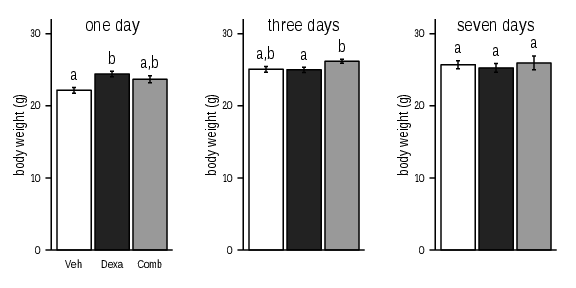
\includegraphics[width=6in,height=3in]{figure/bodyweightsatsacrifice-1} 

\end{knitrout}

\protect\caption[Body weight at sacrifice, following Dexa with / without Testo treatments.]{Body weight at sacrifice, following \SI{10}{\milli\gram\per\kilo\gram\per\day}
Dexa with / without \SI{28}{\milli\gram\per\kilo\gram\per\day} Testo
treatments. Treatments designated by the same letter do not differ
significantly from each other (n=5-6).\label{fig:Body-weight-at-sacrifice}}
\end{figure}


Upon finding the Dexa dose effective in inducing muscle atrophy, I
analyzed the body weight at sacrifice. There was no difference between
groups in terms of absolute weight, due to the large variability of
the initial body weight (Kruskal-Wallis p = 0.777)
(Fig. \ref{fig:Body-weight-at-sacrifice}, right). The difference
became apparent when percent change in body weight was compared (Fig.
\ref{fig:Time-course-of-body-weight}, top, last time point). In this
case, the three treatments (vehicle, Dexa, or the combination Dexa
+ Testo) were significantly different (Kruskal-Wallis p = 0.00385).
Instead of the expected unchanged body weight over the seven days
of treatment with vehicle alone, there was a trend for growth, with
an apparent gain of 0.212
grams every day during the treatment. A similar trend has been seen
in the other repetitions of the experiment, as well as in other published
studies on young rodents. A sizable contribution to this growth was
brought by the \SI{200}{\micro\liter} vehicle injected every day.
Once this artifact is taken into account, the gain of a negligible
0.0333
grams per day in the Dexa-treated group is in fact indicative of an
actual massive loss of body weight.

Seven-day weight gain in Dexa-treated group (1.05
± 1.14\%
of initial body weight) was significantly smaller than that of the
vehicle-treated group (6.12
± 0.879\%;
Dunn's test p = 0.0447).
Conversely, co-administration of Testo, hereafter and in plots abbreviated
\nomenclature{Comb}{combination of Dexa and Testo}, brought back
the body weight gain over seven days to levels similar to those in
vehicle-treated animals (8.62
± 0.674\%;
Dunn's test vs. Dexa alone, p = 0.00167).

\begin{figure}
\begin{knitrout}
\definecolor{shadecolor}{rgb}{0.969, 0.969, 0.969}\color{fgcolor}
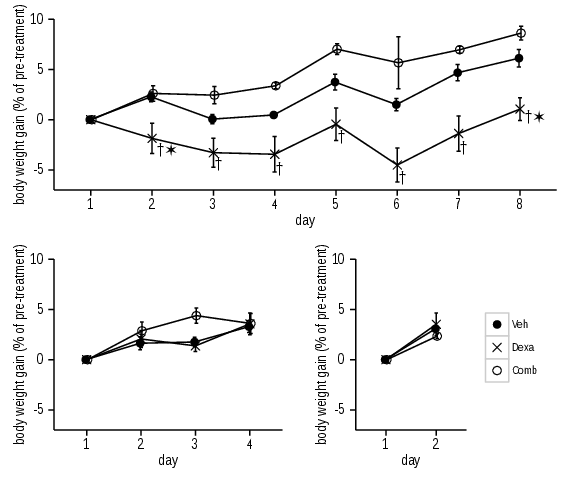
\includegraphics[width=6in,height=5in]{figure/weightcourse-1} 

\end{knitrout}

\protect\caption[Time course of body weight Dexa with / without Testo treatments.]{Time course of body weight Dexa with / without Testo treatments (n=5-6).
Stars indicate statistically significant differences between Veh and
Dexa (p <0.05). Daggers indicate statistically significant differences
between Dexa and Comb (p <0.05).\label{fig:Time-course-of-body-weight}}
\end{figure}


The time course of body weight changes suggested that both drugs'
action had a rapid onset (Fig. \ref{fig:Time-course-of-body-weight};
Kruskal-Wallis for first day percent change in body weight, p = 0.0239).
Specifically, mice receiving vehicle alone gained 2.28
± 0.485\%
body weight in the 24 hours, due to accretion of nonresorbable vehicle.
In contrast, mice receiving Dexa lost 1.86
± 0.485\%
body weight (Dunn's test p = 0.0387).
Mice receiving a combination of Dexa and Testo were essentially indistinguishable
from those receiving vehicle alone, having gained 2.61
± 0.767\%
body weight. This demonstrated an advantage of the combination treatment
over Dexa alone (Dunn's test p = 0.0213).

Based on the whole time course, I hypothesized that body weight changes
and muscle atrophy occur in a gradual manner, with significant metabolic
and molecular changes preceding the seven-day end of experiment. Accordingly,
I repeated the above experiment on different cohorts of mice, which
were sacrificed after only 1 or 3 days of treatment. Once more, absolute
changes in body weight could not be correlated with the muscle changes
(Fig. \ref{fig:Body-weight-at-sacrifice}, left and middle). When
normalized, relative changes in body weight for these groups of mice
were less ample than those seen with 7 days of treatment, to the point
that most parameters (body weight, lean body mass, individual muscles
mass) were not changed in a statistically significant manner (Fig.
\ref{fig:Time-course-of-body-weight}, bottom). These shorter treatments
provided insight into the molecular development of atrophy, but, because
they were run as independent experiments, they will not be analyzed
in conjunction. Because this work is focused on longer-term effects
of Dexa, most of the reported data in the remainder of the section
will be either from mice treated for 7 days with Dexa with / without
Testo, or comparisons of the 1, 3, and 7 day samples.

Body composition analysis indicated that all animals included in these
experiments progressively lost total water. There was no difference
between water loss in the three experimental groups (Fig. \ref{fig:Changes-in-water-lean-and-fat},
top; Kruskal-Wallis for seven day mass of water lost, p = 0.302).
This uniform loss of water negates a scenario in which the observations
could be ascribed to increased water retention due to non-specific
action of either steroid with MR. In all cases, the losses of total
water track the loss of lean body mass, indicating that muscle atrophy,
rather than renal dysfunction, underlies the loss of water. Fat mass
analysis indicated that in the vehicle-alone treated group, the rate
of apparent fat gain was essentially equal with the mass of injected
vehicle accrued over the seven days. This demonstrates that experiments
manipulations, in the absence of pharmacological treatments, have
no effect on lipid metabolism. Dexa-treated mice accrued an additional
0.73
g fat, compared to vehicle (Dunn's test, p = 0.0681.
Similarly, mice treated with the combination accrued 0.922
g additional fat, compared to vehicle (Dunn's test, p = 0.0172).
Therefore, Testo co-administration had no effect on lipid accretion
(Dunn's test, Dexa vs. combination, p = 0.802).

Ampler changes were induced by the two drugs on lean body mass (Fig.
\ref{fig:Changes-in-water-lean-and-fat}, bottom; Kruskal-Wallis for
seven day lost lean mass, p = 0.000811).
Vehicle alone has no effect on lean body mass (0.327
± 0.203 grams lost
over seven days, that is, 1.65\%
of the total lean body mass). Dexa alone induce a massive loss of
lean body mass (3.21
± 0.166 grams lost
over seven days; Dunn's test p = 0.000242).
When Testo was co-administered, the loss of lean body mass persisted,
but there was a trend towards a lower loss rate (1.57
± 0.133 grams lost
over seven days; Dunn's test vs Dexa, p = 0.108).

The loss of lean body mass induced by Dexa was apparent even in the
3-day experiment (1.45
± 0.152 grams lost
over three days; Dunn's test vs. vehicle, p = 0.00961).
Interestingly, in that experiment, Testo protective effect was very
small and not statistically significant (1.28
± 0.369 grams lost
over three days; Dunn's test vs. Dexa, p = 0.675). 

\begin{figure}
\begin{knitrout}
\definecolor{shadecolor}{rgb}{0.969, 0.969, 0.969}\color{fgcolor}
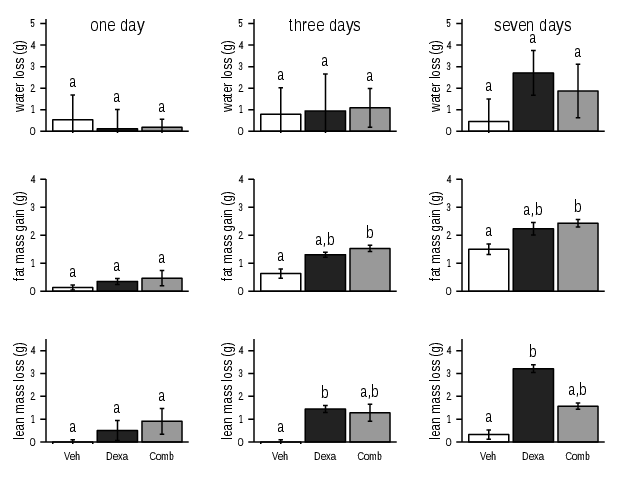
\includegraphics[width=6.5in,height=5in]{figure/leanfat-1} 

\end{knitrout}

\protect\caption[Changes in water, lean, and fat body mass, after Dexa with / without
Testo treatments]{Changes in water, lean, and fat body mass, after Dexa with / without
Testo treatments (n=5-6).\label{fig:Changes-in-water-lean-and-fat}}
\end{figure}


Dissection of individual muscles confirmed that Dexa achieved widespread
muscle atrophy (Fig. \ref{fig:Muscles-weights}). Despite the small
sample size (n=5-6), the atrophying effect of Dexa became statistically
significant at day 3 on gastrocnemius (Dunn's test, p = 0.0369).
At day 7, statistical significance is also achieved in triceps brachii
(Dunn's test, p = 0.0209),
quadriceps (Dunn's test, p = 0.00205),
and levator ani (Dunn's test, p = 0.0245).
In terms of amplitudes, the five measured muscles ranged from extremely
responsive, such as quadriceps (22.7\%
muscle weight loss), triceps (18\%
muscle weight loss) and gastrocnemius (16.5\%
muscle weight loss), to the refractory tibialis anterior (6.2\%
muscle weight loss). For each muscle and time point, the average muscle
weight in the Dexa group was smaller than the average weight of the
controls.

\begin{figure}
\begin{knitrout}
\definecolor{shadecolor}{rgb}{0.969, 0.969, 0.969}\color{fgcolor}
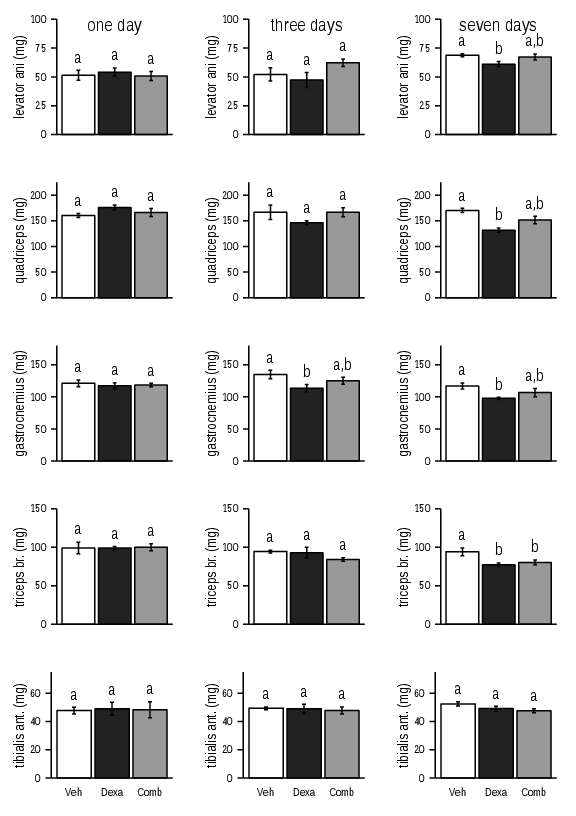
\includegraphics[width=6in,height=8.5in]{figure/muscleweights-1} 

\end{knitrout}

\protect\caption[Effects of Dexa with / without Testo treatments on individual muscle
weights.]{Effects of Dexa with / without Testo treatments on the wet weight
of levator ani, quadriceps, gastrocnemius, triceps brachii, and tibialis
anterior muscles (normalized to body weight; n=5-6).\label{fig:Muscles-weights}}
\end{figure}


Upon Testo co-administration, four out of five muscles measured were
exhibited a trend towards restoration to their basal weight (Fig.
\ref{fig:Muscles-weights}). The amplitude of restorative response
to Testo co-administration was strongest in quadriceps (15.2\%
restoration in muscle weight; Dunn's test, p = 0.27),
followed by levator (10.2\%
restoration in muscle weight; Dunn's test, p = 0.134),
and gastrocnemius (9.07\%
restoration in muscle weight; Dunn's test, p = 0.199)
appear the most responsive.

At the seventh day, Testo co-administration led to an additional 3.12\%
loss in tibialis weight (Dunn's test, p = 0.523).
A similar trend indicating Testo's inability to rescue tibialis mass
is also present in the three-day data (2.63\%
loss; Dunn's test, p =0.975).
The small amplitude and the complete absence of statistical significance
suggest that observations describe lack of Testo effect, rather than
a true atrophic effect. Because tibialis is not manifesting GAML at
macroscopic level, molecular analysis will not include it.

In conclusion, \SI{10}{\milli\gram\per\kilo\gram\per\day} Dexa injection
led to rapid onset of muscle atrophy. Similar to humans with hypercortisolism,
total body weight had limited use in assessing atrophy progression.
Based on the time course of lean body mass and individual muscle changes,
the atrophy develops throughout the first week, indicating that this
murine model replicates chronic GC exposure. Some muscles are more
responsive than others, with tibialis a notable refractory exception.
In contrast, \SI{28}{\milli\gram\per\kilo\gram\per\day} Testo co-administration
reduced the loss of muscle throughout the seven days course. While
rat experiments have described a series of pathways by which Dexa
can achieve muscle atrophy, it was unclear which of them, if any,
is reversed by Testo co-administration.


\section{Testosterone reverses glucocorticoid-induced activation of the ubiquitin-proteasome
system}

The rapid loss of muscle mass induced by Dexa in mice exceeds the
rate of protein turnover in normal adult rodent muscle (about 2.5\%
per day\citep{millward1975skeletal-muscle}). Therefore, Dexa's action
cannot rely exclusively on translational shutdown. I attempted to
establish which protein degradative pathways could be mediating the
atrophic effect of dexamethasone. Experiments on rats suggest that
Dexa causes protein degradation by stimulating the proteasome-ubiquitin-related
transcriptional program, whereas Testo represses it.

In normal circumstances, the rate-limiting factor in proteasome-mediated
protein degradation is target protein conjugation with ubiquitin,
catalyzed by E3 ligases. In mice treated with Dexa, the E3 ligase
more commonly associated with loss of muscle mass, MuRF-1 (Fig. \ref{fig:Atrogenes-expression},
top), was upregulated by Dexa at day 1 in gastrocnemius (1.9-fold
amplification; Dunn's test, p = 0.116)
and in quadriceps (61.5-fold
amplification; Dunn's test, p = 0.00906).
The effect was even more consistent at day 3, with MuRF-1 transcript
in gastrocnemius being 7.58-fold
amplified (Dunn's test, p =0.0154),
and in quadriceps 4.71-fold
amplified (Dunn's test, p =0.0726).
The effect was insignificant statistically, and in amplitude, by the
seventh day of Dexa administration.

Testo co-administration had an inhibitory effect on MuRF-1, with a
later onset. No significant effect of Testo co-administration was
seen in day 1. In day 3 samples, MuRF-1 was repressed by Testo in
gastrocnemius (1.97-fold
reduction; Dunn's test, p =0.591)
and in quadriceps (5.82-fold
reduction; Dunn's test, p =0.0268).
Testo repression of MuRF-1 strengthened in the day 7 samples, with
transcripts reduced in gastrocnemius (2.11
fold reduction; Dunn's test, p = 0.116)
and in quadriceps (2.13
fold reduction; Dunn's test, p = 0.0748).

\begin{figure}
\begin{knitrout}
\definecolor{shadecolor}{rgb}{0.969, 0.969, 0.969}\color{fgcolor}
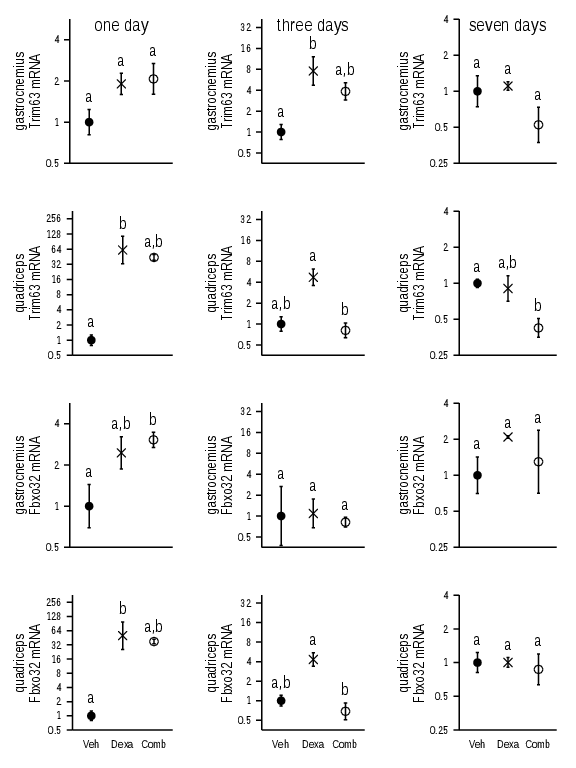
\includegraphics[width=6in,height=8in]{figure/atrogenes-1} 

\end{knitrout}

\protect\caption[Changes in atrogenes MuRF-1 / Trim63 and MAFbx / Fbxo32 expression
following Dexa with / without Testo treatments]{Changes in atrogenes MuRF-1 / Trim63 and MAFbx / Fbxo32 expression
following Dexa with / without Testo treatments, in quadriceps and
gastrocnemius muscles (n=3-5, normalized to GAPDH).\label{fig:Atrogenes-expression}}
\end{figure}


A similar pattern, although with lower intensity, was seen in MAFbx
gene regulation by the two steroids. MAFbx was reliably upregulated
by Dexa at day 1 in gastrocnemius (2.45
fold amplification; Dunn's test, p = 0.175)
and quadriceps (50.1
fold amplification; Dunn's test, p = 0.00906).
At day 3, only the quadriceps MAFbx response was still present to
a significant degree (4.32
fold amplification; Dunn's test, p = 0.113).
The effect became insignificant statistically across muscle groups
by the seventh day of Dexa administration.

Testo co-administration had no statistically significant effect on
MAFbx at days 1 and 7. By day 3, MAFbx was repressed by Testo in gastrocnemius
(1.34
fold amplification; Dunn's test, p = 0.616)
and in quadriceps (6.29
fold amplification; Dunn's test, p = 0.0154).

The other component of the ubiquitin-proteasome system is the proteasome
itself. In cases where E3 ligases are upregulated, it may be the case
that availability of proteasomes is limiting the ubiquitin-proteasome
system. However, in day 3 samples, where atrogene upregulation was
at its peak, Dexa upregulated proteasome chymotrypsin-like enzymatic
activity in quadriceps (18.7\%
increase; Dunn's test, p = 0.157)
and triceps (111\%
increase; Dunn's test, p = 0.0884;
Fig. \ref{fig:Proteasome-enzymatic-activity}). This component of
atrophy was also inhibited by Testo, whose co-administration reduced
proteasome activity in quadriceps (24.2\%
reduction; Dunn's test, p = 0.435)
and triceps (30\%
reduction; Dunn's test, p = 0.609)
at day 3.

\begin{figure}
\begin{knitrout}
\definecolor{shadecolor}{rgb}{0.969, 0.969, 0.969}\color{fgcolor}
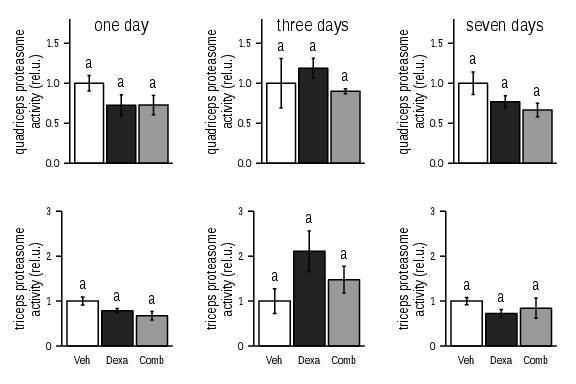
\includegraphics[width=6in,height=4in]{figure/proteasomeactivity-1} 

\end{knitrout}

\protect\caption[Changes in proteasome enzymatic activity following Dexa with / without
Testo treatments.]{Changes in proteasome chymotrypsin-like enzymatic activity following
Dexa with / without Testo treatments, in quadriceps and triceps muscles
(n=4-6).\label{fig:Proteasome-enzymatic-activity}}
\end{figure}


Overall, the good correlation with the macroscopic loss of muscle
suggests that the proteasome-ubiquitin system is an effector of GAML
and a target of its alleviation by AAS.


\section{Autophagy markers during dexamethasone and testosterone treatments}

Rat microarray studies indicated that a series of genes related to
autophagy are upregulated by Dexa and downregulated by Testo. However,
these findings have never been tested in vivo in mice. Having established
a model of GAML, I investigated whether the autophagy markers are
correlated with muscle loss. A panel of three genes indicated that
Dexa-induced gastrocnemius atrophy is associated with a reduction
in autophagy-related transcription (Fig. \ref{fig:Autophagy-related-genes})
The repression is ampler in day 3 samples, with mRNA for beclin /
Becn1 reduced 9.81-fold
(Dunn's test, p = 0.0213),
cathepsin L / Ctsl reduced 3.89-fold
(Dunn's test, p = 0.304),
and LC3 / Map1lc3b reduced 5.61-fold
(Dunn's test, p = 0.359).
Across muscle groups and time points, Testo co-administration lacked
detectable effect.

\begin{figure}
\begin{knitrout}
\definecolor{shadecolor}{rgb}{0.969, 0.969, 0.969}\color{fgcolor}
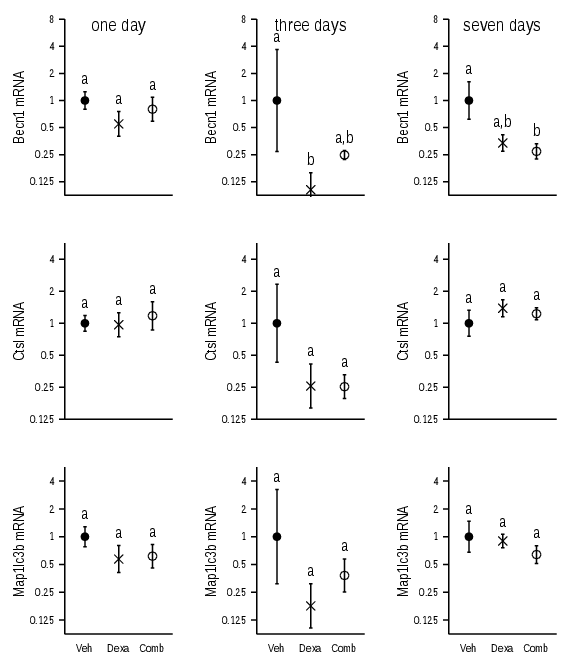
\includegraphics[width=6in,height=7in]{figure/gastrocnemiusautophagy-1} 

\end{knitrout}

\protect\caption[Changes in autophagy-related genes following Dexa with / without Testo
treatments.]{Changes in autophagy-related genes following Dexa with / without
Testo treatments, in quadriceps and triceps muscles (n=3-4, normalized
to GAPDH).\label{fig:Autophagy-related-genes}}
\end{figure}


I tested the hypothesis that autophagy mediates protein degradation
in GAML by measuring lysosome enzymatic activity in muscle lysates
(Fig. \ref{fig:Cathepsin-enzymatic-activity}). Unexpectedly, cathepsin
L enzymatic activity was reduced in all the assayed muscle, in a progressive
manner. At day 1, cathepsin L activity was suppressed by Dexa in gastrocnemius
(16.4\%
reduction; Dunn's test, p = 0.02),
quadriceps (14.5\%
reduction; Dunn's test, p = 0.0294),
and triceps (26.8\%
reduction; Dunn's test, p = 0.00219).
At day 3, cathepsin L activity was further suppressed by Dexa in gastrocnemius
(19.7\%
reduction; Dunn's test, p = 0.223),
quadriceps (44.5\%
reduction; Dunn's test, p = 0.00201),
and triceps (44.5\%
reduction; Dunn's test, p = 0.00107).
In day 7 samples, Dexa-induced repression of cathepsin L activity
reached 36.3\%
in gastrocnemius (Dunn's test, p = 0.00365),
44.4\%
in triceps (Dunn's test, p = 0.0486),
and 44.9\%
in quadriceps (Dunn's test, p = 0.0091).
Testo co-administration had no statistically significant effect on
cathepsin L enzymatic activity, although a trend of reversal to baseline
can be seen in day 1 and 3 samples.

\begin{figure}
\begin{knitrout}
\definecolor{shadecolor}{rgb}{0.969, 0.969, 0.969}\color{fgcolor}
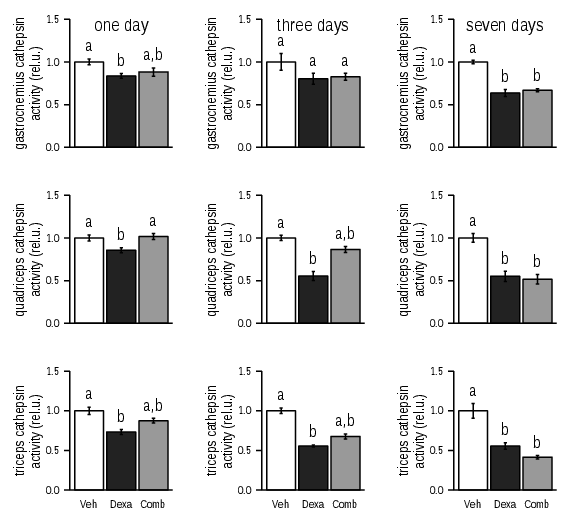
\includegraphics[width=6in,height=5.5in]{figure/cathepsinactivity-1} 

\end{knitrout}

\protect\caption[Changes in cathepsin enzymatic activity following Dexa with / without
Testo treatments.]{Changes in cathepsin L enzymatic activity following Dexa with / without
Testo treatments, in quadriceps and triceps muscles (n=4-6).\label{fig:Cathepsin-enzymatic-activity}}
\end{figure}


In literature, another line of evidence for the putative upregulation
of autophagy during GAML was the increase in lipidated, fast migrating
LC3 protein (also known as LC3-II). In murine muscle, detecting this
form has been difficult, because it is significantly less frequent
than its slower migrated counterpart (Fig. \ref{fig:LC3-hyperlipidated}).
In gastrocnemius at day 7, there was a trend towards enrichment of
LC3-II in absolute terms upon Dexa treatment (91.6\%
increase, when normalized to GAPDH; Dunn's test, p = 1).
However, LC3-II changes become negligible, when LC3-II is normalized
to its precursor, LC3-I (-0.339\%
increase; Dunn's test, p = 1).

\begin{figure}
\begin{minipage}[t][2in][c]{3in}%
\includegraphics[width=3in]{1_media_dump_writingswork_draftthesis_artwork_lc3-gastroc_lc3-gastroc.pdf}%
\end{minipage}%
\begin{minipage}[t][2.2in][c]{3in}%
\begin{knitrout}
\definecolor{shadecolor}{rgb}{0.969, 0.969, 0.969}\color{fgcolor}
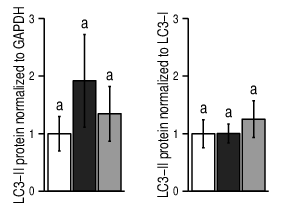
\includegraphics[width=3in,height=2.in]{figure/lcprotein-1} 

\end{knitrout}
%
\end{minipage}

\protect\caption[Changes in LC3 lipidation status following Dexa with / without Testo
treatments.]{Changes in hyperlipidated (fast-migrating) LC3 isoform following
Dexa with / without Testo treatment in gastrocnemius muscles (n=4)\label{fig:LC3-hyperlipidated}.}
\end{figure}


The trend towards increased absolute LC3-II in gastrocnemius is reversed
by a trend towards basal levels upon Testo co-administration (29.8\%
decrease, when normalized to GAPDH; Dunn's test, p = 1).

\begin{figure}
\begin{knitrout}
\definecolor{shadecolor}{rgb}{0.969, 0.969, 0.969}\color{fgcolor}
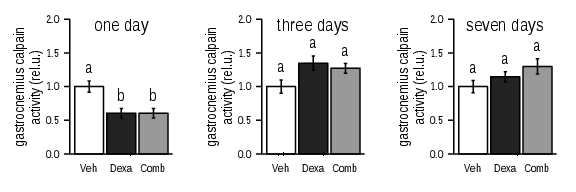
\includegraphics[width=6in,height=2in]{figure/calpainactivity-1} 

\end{knitrout}

\protect\caption[Calpain enzymatic activity during Dexa with / without Testo treatments.]{μ-calpain enzymatic activity, during 7 days of Dexa with / without
Testo treatments, in gastrocnemius muscles (n=3-6).\label{fig:Calpain-enzymatic}}


\end{figure}


Findings like the upregulation of LC3-II may have suggested to other
authors that GAML relies on autophagy. However, the overall evidence
suggests that GAML is correlated with rampant autophagy downregulation,
while AAS co-administration has a limited effect on autophagy. Immunoblots
and enzymatic assays indicated a similar disconnection between the
calpain / calpastatin system and the AAS-induced muscle sparing (Fig.
\ref{fig:Calpain-enzymatic}). The ubiquitin - proteasome system emerges
as the main effector of GAML and the main target of its alleviation
by AAS, in this model system.


\section{Protein synthesis modulation during Dexa-induced muscle atrophy}

Often, literature reports describe how upregulation of muscle catabolism
following Dexa treatments is compounded by repression of protein synthesis.
In order to discern putative changes in protein synthesis in this
model, I investigated a series of its translation regulators. A well-documented
manner of translational shutdown upon various conditions, such as
endoplasmic reticulum stress, is phosphorylation of the initiation
factor eIF2α by a diverse set of kinases. In agreement with published
studies, there was no statistically significant change in phospho-eIF2α
in the gastrocnemius of mice treated with Dexa (Dunn's test, p = 1;
Fig. \ref{fig:Phosphorylated-eif2}). 

\begin{figure}
\begin{minipage}[t][2in][c]{3in}%
\includegraphics[width=3in]{2_media_dump_writingswork_draftthesis_artwork_eif2blot_phosphoeif2-blot.pdf}%
\end{minipage}%
\begin{minipage}[t][2.2in][c]{3in}%
\begin{knitrout}
\definecolor{shadecolor}{rgb}{0.969, 0.969, 0.969}\color{fgcolor}
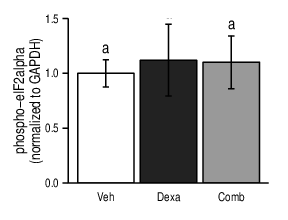
\includegraphics[width=3in,height=2.in]{figure/eiftwo-1} 

\end{knitrout}
%
\end{minipage}

\protect\caption[Levels of phosphorylated eIF2α following Dexa with / without Testo
treatments.]{Levels of phosphorylated eIF2α (Ser 51) following Dexa with / without
Testo treatment in gastrocnemius muscles (normalized to simultaneously
resolved GAPDH; n=4)\label{fig:Phosphorylated-eif2}.}
\end{figure}


Another regulator of proteins synthesis that was shown to play a role
in muscle atrophy upon starvation is eIF3f. In levator muscles of
mice treated with Dexa, there was no statistically significant change
in the levels of eIF3f (Dunn's test, p = 0.971;
Fig. \ref{fig:eif3f}).

\begin{figure}
\begin{minipage}[t][2in][c]{3in}%
\includegraphics[width=3in]{3_media_dump_writingswork_draftthesis_artwork_eif3fblot_eif3-blot.pdf}%
\end{minipage}%
\begin{minipage}[t][2.2in][c]{3in}%
\begin{knitrout}
\definecolor{shadecolor}{rgb}{0.969, 0.969, 0.969}\color{fgcolor}
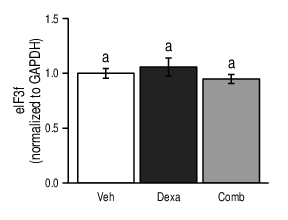
\includegraphics[width=3in,height=2.in]{figure/eifthree-1} 

\end{knitrout}
%
\end{minipage}

\protect\caption[Levels of eIF3f following Dexa with / without Testo treatments.]{Levels of eIF3f following Dexa with / without Testo treatment in
levator ani muscles (normalized to simultaneously resolved GAPDH;
n=4)\label{fig:eif3f}.}
\end{figure}


Finally, Dexa was hypothesized to achieve protein synthesis inhibition
by stimulating the negative regulator 4E-BP. In Dexa-treated mice,
gastrocnemius 4E-BP protein levels were upregulated (25.6\%
increase, when normalized to GAPDH; Dunn's test, p = 0.428;
Fig. \ref{fig:4EBP}, left). However, Dexa also stimulated phosphorylated,
that is, inactive 4E-BP (62.5\%
increase, when normalized to GAPDH; Dunn's test, p = 0.00669;
Fig. \ref{fig:4EBP}, right). The effect of Dexa on active, that is,
unphosphorylated 4E-BP could not be clearly estimated from these immunoblot
data.

\begin{figure}
\begin{minipage}[t][2in][c]{6in}%
\includegraphics[width=6in]{4_media_dump_writingswork_draftthesis_artwork_4eBP_4eBP.pdf}%
\end{minipage}

\begin{minipage}[t][2.2in][c]{6in}%
\begin{knitrout}
\definecolor{shadecolor}{rgb}{0.969, 0.969, 0.969}\color{fgcolor}
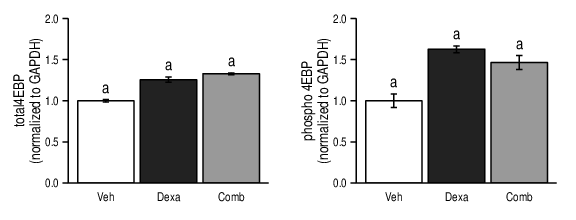
\includegraphics[width=6in,height=2.3in]{figure/fourebp-1} 

\end{knitrout}
%
\end{minipage}

\protect\caption[Levels of total and phosphorylated 4E-BP following Dexa with / without
Testo treatments.]{Levels of total (left) and phosphorylated (right) 4E-BP following
Dexa with / without Testo treatment in gastrocnemius muscles (normalized
to GAPDH; n=4)\label{fig:4EBP}.}
\end{figure}


After 7 days of Testo co-administration, levels of total 4E-BP were
essentially identical to those yielded by Dexa alone (5.6\%
increase; Dunn's test, p = 0.428;
Fig. \ref{fig:4EBP}, right). At the same time, Testo co-administration
was associated with lower phosphorylated 4E-BP (9.83\%
increase, when normalized to GAPDH; Dunn's test, p = 0.49;
Fig. \ref{fig:4EBP}, left). The combination of increase in total
4E-BP and decrease in inactivated 4E-BP suggests an unexpected increase
in active 4E-BP, which could have led to reduction in the rate of
protein synthesis. The amplitude of Testo-induced changes in 4E-BP
is small, and the direction opposite to what would be required to
upregulate protein synthesis and facilitate muscle recovery.

Overall, regulators of protein synthesis appeared largely unchanged
by Testo at the 7-day stage of their administration, in this model
system.


\section{Foxo pathway response to dexamethasone and testosterone}

Previous studies on C2C12 cultured cells showed that the atrogene
response is crucially stimulated by Foxo transcription factors. The
review section describes a series of five hypothetical means by which
Dexa is thought to stimulate Foxo transcriptional program. Most of
them converge on upregulation of Foxo transcripts. I set to test the
hypothesis that muscle Foxo expression is modulated by Dexa and Testo
in muscle.

In this study, Foxo transcription factors were strongly induced during
the early stages of GAML (Fig. \ref{fig:Foxo-expression}). In quadriceps
at day 1, Foxo3a RNA was 78.1-fold
upregulated (Dunn's test, p = 0.00906).
In day 3 samples, Foxo3a activation was less ample (3.17-fold;
Dunn's test, p = 0.0529).
In the samples from day 7, Dexa treatment was associated with a non-significant
downregulation of Foxo3a (Dunn's test, p = 0.175).

\begin{figure}
\begin{knitrout}
\definecolor{shadecolor}{rgb}{0.969, 0.969, 0.969}\color{fgcolor}
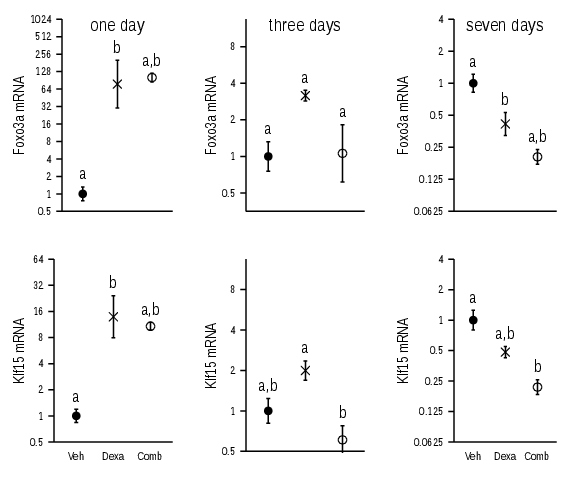
\includegraphics[width=6in,height=5in]{figure/foxogene-1} 

\end{knitrout}

\protect\caption[Changes in the expression of Foxo3a and Klf15 transcription factors
during Dexa with / without Testo treatments.]{Changes in the expression of Foxo3a (top) and Klf15 (bottom) transcription
factors, during 7 days of Dexa with / without Testo treatments in
quadriceps muscles (n=4, normalized to GAPDH).\label{fig:Foxo-expression}}


\end{figure}


In contrast, Testo downregulated Foxo transcription factors at later
stages of GAML. In day 3 samples, Testo co-administration repressed
Foxo3a 2.99-fold
(Dunn's test, p = 0.195).
The trend was present in day 7 samples too, with Foxo3a repressed
2.04-fold
(Dunn's test, p = 0.304)
by Testo co-administration. Similar patterns of modulation were seen
in Foxo1 and Foxo4 transcripts (data not shown).

The changes in Foxo transcription factors were mirrored by similar
changes in their positive regulator Klf15. Dexa stimulated Klf15 expression
at day 1 (13.9-fold
upregulation; Dunn's test, p = 0.00906),
and day 3 (2-fold
upregulation; Dunn's test, p = 0.222).
Testo co-administration reversed Klf15 changes, with the strongest
repression, 3.28-fold,
in day 3 samples (Dunn's test, p = 0.017).


\section{Akt pathway response to dexamethasone and testosterone}

An alternative way to achieve Foxo modulation is through their neutralization
by Akt. As described in the literature review section, activation
of Akt is dependent on its phosphorylation on two residues, Ser 473
and Thr 308, with the former being the most important regulator of
Foxo specificity. I therefore investigated the effect of the two steroids
on Ser 473 phosphorylation.

\begin{figure}
\begin{minipage}[t][1.8in][c]{6in}%
\includegraphics[width=6in,height=1.8in]{5_media_dump_writingswork_draftthesis_artwork_Akt_Akt-gastroc.pdf}%
\end{minipage}

\begin{minipage}[t][2.2in][c]{6in}%
\begin{knitrout}
\definecolor{shadecolor}{rgb}{0.969, 0.969, 0.969}\color{fgcolor}
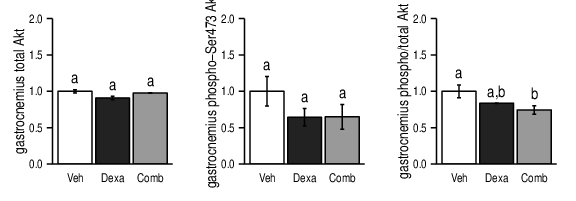
\includegraphics[width=6in,height=2.1in]{figure/gastrocnemiusakt-1} 

\end{knitrout}
%
\end{minipage}

\begin{minipage}[t][1.8in][c]{6in}%
\includegraphics[width=6in,height=1.8in]{6_media_dump_writingswork_draftthesis_artwork_Akt_Akt-levator.pdf}%
\end{minipage}

\begin{minipage}[t][2.2in][c]{6in}%
\begin{knitrout}
\definecolor{shadecolor}{rgb}{0.969, 0.969, 0.969}\color{fgcolor}
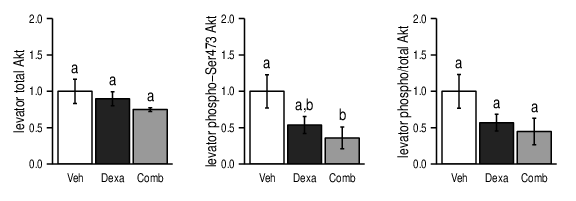
\includegraphics[width=6in,height=2.1in]{figure/levatorakt-1} 

\end{knitrout}
%
\end{minipage}

\protect\caption[Levels of total and phosphorylated Akt following Dexa with / without
Testo treatments.]{Levels of total and phosphorylated Akt following 7 days of Dexa with
/ without Testo treatment in gastrocnemius (top) and levator (bottom)
muscles (normalized to GAPDH; n=4)\label{fig:Akt-phosphorylation}.}
\end{figure}


After 7 days, neither drug changed the level of total Akt in levator,
nor gastrocnemius (Fig. \ref{fig:Akt-phosphorylation}, left). At
the same time, Dexa repressed phosphorylation of a large degree in
gastrocnemius (35.6\%
reduction in absolute densitometry of phospho-Ser473 Akt, when normalized
to GAPDH; Dunn's test, p = 0.304),
and levator ani (46.2\%
reduction; Dunn's test, p = 0.146).
However, Testo co-administration had no significant effect on phospho-Ser473
Akt in gastrocnemius (0.842\%
increase, p = 1).
Interestingly, in this model system, Testo co-administration repressed
phospho-Ser473 in levator ani, an extremely AAS-sensitive muscle (33.1\%
decrease; Dunn's test, p = 0.823).

The other relevant phosphorylation on Akt, Thr 308, is controlled
by REDD1. I investigated the effects of the two steroids on REDD1
/ Ddit4 transcription (fig. \ref{fig:Redd1-expression}). Dexa upregulated
Redd1 expression in gastrocnemius collected at days 1 (7.48-fold;
Dunn's test, p = 0.0362),
3 (27.8-fold;
Dunn's test, p = 0.0912),
and 7 (2.64-fold;
Dunn's test, p = 0.255).
Confirming the rat microarray studies, at day 7, Testo co-administration
induced a sizable repression of REDD1 (1.85-fold;
Dunn's test, p = 0.143).

\begin{figure}
\begin{knitrout}
\definecolor{shadecolor}{rgb}{0.969, 0.969, 0.969}\color{fgcolor}
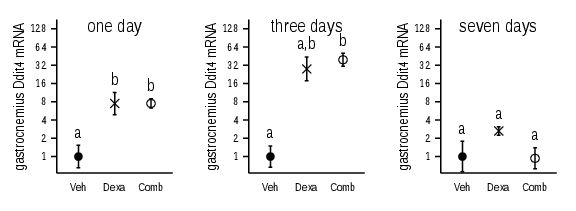
\includegraphics[width=6in,height=2.2in]{figure/redd-1} 

\end{knitrout}

\protect\caption[Changes in the expression of Redd1 during Dexa with / without Testo
treatments.]{Changes in Redd1 transcripts, during 7 days of Dexa with / without
Testo treatments in gastrocnemius muscles (n=4, normalized to GAPDH).\label{fig:Redd1-expression}}
\end{figure}



\section{IGF-I changes during dexamethasone and testosterone administration}

As explained in the review section, IGF-I was one of the few genes
whose expression was changed in opposite ways by Dexa and Testo in
rat microarrays. I tested the hypothesis that Dexa and Testo alter
IGF-I expression in mice, in vivo (Fig. \ref{fig:Igf1-expression}).

\begin{figure}
\begin{knitrout}
\definecolor{shadecolor}{rgb}{0.969, 0.969, 0.969}\color{fgcolor}
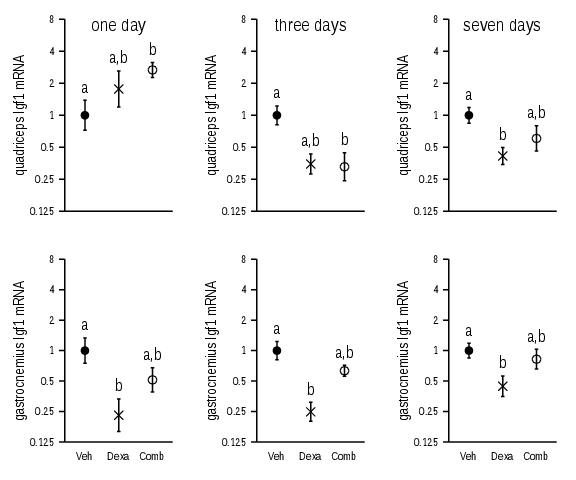
\includegraphics[width=6in,height=5in]{figure/Igf-1} 

\end{knitrout}

\protect\caption[Changes in the expression of IGF-I during Dexa with / without Testo
treatments.]{Changes in the expression of IGF-I, during 7 days of Dexa with /
without Testo treatments in gastrocnemius muscles (n=4, normalized
to GAPDH).\label{fig:Igf1-expression}}
\end{figure}
 In gastrocnemius, Dexa downregulated IGF-I expression in samples
collected at days 1 (4.35-fold;
Dunn's test, p = 0.0213),
3 (4.03-fold;
Dunn's test, p = 0.0105),
and 7 (2.25-fold;
Dunn's test, p = 0.0362).
Dexa-induced downregulation of IGF-I was also detected in quadriceps
at days 3 (2.87-fold;
Dunn's test, p = 0.0319),
and 7 (2.41-fold;
Dunn's test, p = 0.0213).

Testo reliably reversed this change. In gastrocnemius, Dexa downregulated
IGF-I expression in samples collected at days 1 (2.23-fold;
Dunn's test, p = 0.421),
3 (2.55-fold;
Dunn's test, p = 0.0825),
and 7 (1.85-fold;
Dunn's test, p = 0.175).
A similar trend was seen in quadriceps, but the amplitude was smaller,
perhaps owing to the fact that Dexa-induced changed in IGF-I were
smaller.

Throughout this section, the molecular correlates of GAML, as found
in rats, were confirmed in this novel mouse model. However, few of
the effects of Dexa were reversed by Testo, at the resolution of my
experimental design. However, among the putative mechanisms of alleviation
of GAML, there is good evidence for the repression of the proteasome
- ubiquitin system and for restoration of intramuscular IGF-I. In
the next section, I describe my efforts to better understand these
myoprotective mechanisms, using an in vitro model. \pagebreak{}


\chapter{In vitro findings}


\section{Testosterone alleviates dexamethasone-induced atrophy of cultured
cells}

In mouse explanted myofibers and C2C12 cultured myotubes, muscle atrophy
is a cell-autonomous phenomenon, with all its essential manifestations
present in vitro. I hypothesized that the muscle protection by Testo
could be replicated in C2C12 cells. Indeed, fully differentiated C2C12
myotubes treated for \SI{48}{\hour} with \SI{50}{\micro\molar} Dexa
lost 8.66\%
in diameter (Tukey's HSD, p = 0.000316).
Co-administration of \SI{300}{\nano\molar} Testo re-established basal
diameters (Tukey's HSD vs. Dexa alone, p = 1.02e-05).

\begin{figure}
\begin{minipage}[t][2.3in][c]{3in}%
\includegraphics[width=3in]{7_media_dump_writingswork_draftthesis_artwork_diameters_Rhodamine_vv-1_001_cr.png}

(Veh)%
\end{minipage}%
\begin{minipage}[t][2.3in][c]{3in}%
\includegraphics[width=3in]{8_media_dump_writingswork_draftthesis_artwork_diameters_Rhodamine_dd-1_001_cr.png}

(Dexa)%
\end{minipage}

\begin{minipage}[t][2.3in][c]{3in}%
\includegraphics[width=3in]{9_media_dump_writingswork_draftthesis_artwork_diameters_Rhodamine_xx-2_001_cr2.png}

(Dexa + Testo)%
\end{minipage}%
\begin{minipage}[t][2.2in][c]{6in}%
\begin{knitrout}
\definecolor{shadecolor}{rgb}{0.969, 0.969, 0.969}\color{fgcolor}
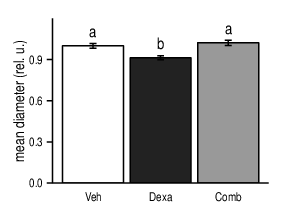
\includegraphics[width=3in,height=2.3in]{figure/celldiams-1} 

\end{knitrout}
%
\end{minipage}

\protect\caption[Changes in C2C12 myotube diameter following Dexa with / without Testo
treatments.]{Changes in C2C12 myotube diameter following Dexa with / without Testo
treatments. Micrographs are representative for cells receiving (top
left) vehicle, or (top right) \SI{50}{\micro\molar} Dexa, or (bottom
left) \SI{50}{\micro\molar} Dexa and \SI{300}{\nano\molar} Testo.
Bottom right image compares average myotube diameters for the three
treatments (n=510-740).\label{fig:myotube-diameters}}
\end{figure}


In another experiment, I tested the ability of Testo to preserve protein
content in C2C12 cells. In order to determine the time course of protein
content, cells were treated with (A) vehicle, (B) \SI{1}{\micro\molar}
Dexa, (C) \SI{1}{\micro\molar} Dexa and \SI{100}{\nano\molar} Testo,
or (D) \SI{1}{\micro\molar} Dexa and \SI{500}{\nano\molar} Testo,
for up to three days, in increments of \SI{24}{\hour} (Fig. \ref{fig:protein-mass-cells},
top). All the treatments led to loss of total protein starting from
the third day, presumably due to senescence and / or loss of viability
(ANOVA treatment x time, p = 0.000463
for time variable). When all the samples were analyzed together, treatment
had no significant effect (ANOVA treatment x time, p = 0.0943
for treatment variable).

However, there were differences in total protein density prior to
the third day, which mimicked the in vivo findings. These trends become
apparent when data is represented after normalization to the initial
time point (Fig. \ref{fig:protein-mass-cells}, top), or when data
is analyzed only across days 1-3. In the first two days, there were
no relevant changes in total protein content in cells treated with
vehicle. Total protein concentration was 81.8
\si{\micro\gram\per\centi\meter\squared} in the first day, 81.1
\si{\micro\gram\per\centi\meter\squared} in the second, and 81.6
\si{\micro\gram\per\centi\meter\squared} in the third (ANOVA p =
0.957).
In contrast, Dexa-treated cells lost protein, declining from 83.3
\si{\micro\gram\per\centi\meter\squared} in the first day to 81.4
\si{\micro\gram\per\centi\meter\squared} in the second and 78.9
\si{\micro\gram\per\centi\meter\squared} in the third day of the
experiment (5.32\%
loss; ANOVA p = 0.957).
Co-administration of Testo more than compensated the effect of Dexa.
Rather than losing protein, cells receiving a combination of \SI{1}{\micro\molar}
Dexa and \SI{100}{\nano\molar} Testo gained 4.99
\% total protein over the first two days of the experiment (ANOVA
p = 0.957).
Moreover, increasing the Testo dose to \SI{500}{\nano\molar} further
improved protein accretion, leading to a 7.16
\% protein gain during the first two days of the experiment (ANOVA
p = 0.957).

\begin{figure}
\begin{knitrout}
\definecolor{shadecolor}{rgb}{0.969, 0.969, 0.969}\color{fgcolor}
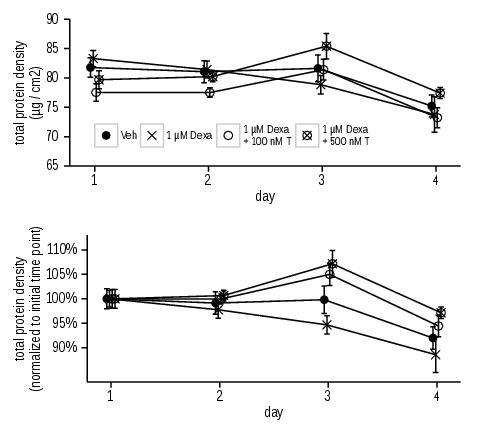
\includegraphics[width=5in,height=4.5in]{figure/totalprotein-1} 

\end{knitrout}

\protect\caption[Changes in C2C12 myotube protein content following Dexa with / without
Testo treatments.]{Changes in C2C12 myotube total protein content following Dexa with
/ without Testo treatments (Top) Absolute total protein density. (Bottom)
The same data, after normalization to the average of the initial time
point for each condition (n=5-6).\label{fig:protein-mass-cells}}
\end{figure}


Overall, the changes in cell diameter and total protein content are
similar to changes observed in muscle in vivo.


\section{Protein synthesis in cultured cells treated with dexamethasone and
testosterone}

In preliminary experiments, I found that tracer uptake is minimal
during the first two hours. In addition, tracer uptake rate became
essentially equal to the rate of tracer release due to protein synthesis
after the first \SI{18}{\hour} of labeling. Therefore, I performed
a series of assays where the rate of protein synthesis was estimated
through the rate of tracer uptake over an intermediate \SI{6}{\hour}
(Fig. \ref{fig:protein-synthesis-cells}, top). In each case, cells
were differentiated over seven days, then treated with (A) vehicle,
(B) \SI{1}{\micro\molar} Dexa, or (C) \SI{1}{\micro\molar} Dexa
and \SI{500}{\nano\molar} Testo, for either 6, 24, 48, or 72 hours.
The media with steroids was refreshed every 24 hours. The tracer was
added with a final medium change, six hours before lysis.

\begin{figure}
\begin{minipage}[t][3.3in]{6in}%
\includegraphics[width=6in]{10_media_dump_writingswork_draftthesis_artwork_cell-labeling-synthesis.pdf}%
\end{minipage}

\begin{minipage}[t][4.5in][c]{6in}%
\begin{knitrout}
\definecolor{shadecolor}{rgb}{0.969, 0.969, 0.969}\color{fgcolor}
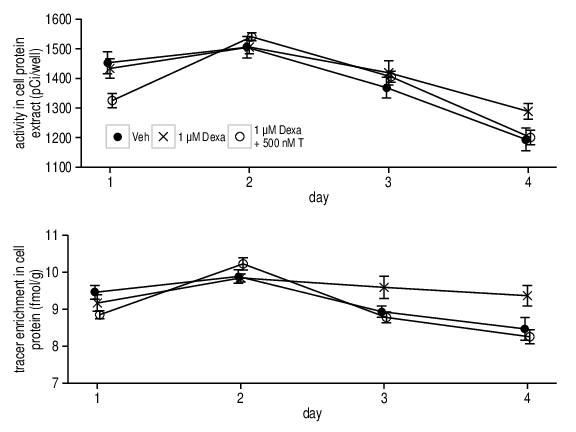
\includegraphics[width=6in,height=4.5in]{figure/proteinsynthesis-1} 

\end{knitrout}
%
\end{minipage} 

\protect\caption[Estimates of protein synthesis rate in C2C12 myotubes treated with
Dexa with / without Testo.]{Estimates of protein synthesis rate in C2C12 myotubes treated with
Dexa with / without Testo. (Top) Experimental timeline. (Middle) Amount
of tracer incorporated into protein per well. (Bottom) Amount of tracer
incorporated into protein per gram of total protein (n=6). \label{fig:protein-synthesis-cells}}
\end{figure}


After lysis, cells were assayed for protein-bound tracer. There was
no effect of treatment on the amount of tracer taken up by the cells
(Fig. \ref{fig:protein-synthesis-cells}, middle). To avoid the confounding
influence of the atrophy, data was also analyzed as specific activity,
that is, protein-bound intracellular tracer normalized to the mass
of cell protein (Fig. \ref{fig:protein-synthesis-cells}, bottom).
The same qualitative observations could be made after normalization.
There was a significant effect of time on the rate of protein synthesis
(ANOVA treatment x time, p = 2.45e-08
for time variable). The time variable was significant due to a downward
trend form days 2 through 4. This trend adds to the notion that C2C12
fully differentiated myotubes quickly lose their viability. When all
the samples were analyzed together, treatment had no significant effect
(ANOVA treatment x time, p = 0.302
for treatment variable). There is no statistically significant difference
between treatments at each time point. The amplest difference in translation
rate between treatments is in day 4, when, in Dexa cells, protein
synthesis rate is higher than in all other conditions (specific activity
10.6\%
higher than vehicle, and 13.5\%
higher than the combination with testosterone). The trend toward increased
protein synthesis with Dexa cannot explain the observed myotube atrophy
induced by Dexa. Moreover, the late onset of protein synthesis upregulation
indicates that this may be a compensatory response to the earlier
loss of protein.

Within the limits of the C2C12 model utilized in these experiments,
protein synthesis changes do not appear to mediate Dexa-induced loss
of protein, nor its alleviation by Testo.


\section{Testosterone prevents protein catabolism upregulation induced by
dexamethasone}

A series of complementary experiments estimated the rate of protein
degradation in C2C12 myotubes. In each case, cells were differentiated
over seven days, then treated with (A) vehicle, (B) \SI{1}{\micro\molar}
Dexa, (C) \SI{1}{\micro\molar}  Dexa and \SI{100}{\nano\molar} Testo,
or (D) \SI{1}{\micro\molar} Dexa and \SI{500}{\nano\molar} Testo,
for either 6, 24, 48, or 72 hours (Fig. \ref{fig:protein-degradation-cells},
top). The media with steroids was refreshed every 24 hours. The tracer
was added three days before the addition of steroids, and was maintained
in the media until 6 hours before lysis. Because the rate of incorporation
of tracer slows down before the first 24 hours, and therefore it may
be assumed that, with some approximation, the ratio of tracer to tracee
in culture medium is equal to that in the pool of rapid-turnover intracellular
protein.

\begin{figure}
\begin{minipage}[t][3.3in]{6in}%
\includegraphics[width=6in]{11_media_dump_writingswork_draftthesis_artwork_cell-labeling-degradation.pdf}%
\end{minipage}

\begin{minipage}[t][4.5in][c]{6in}%
\begin{knitrout}
\definecolor{shadecolor}{rgb}{0.969, 0.969, 0.969}\color{fgcolor}
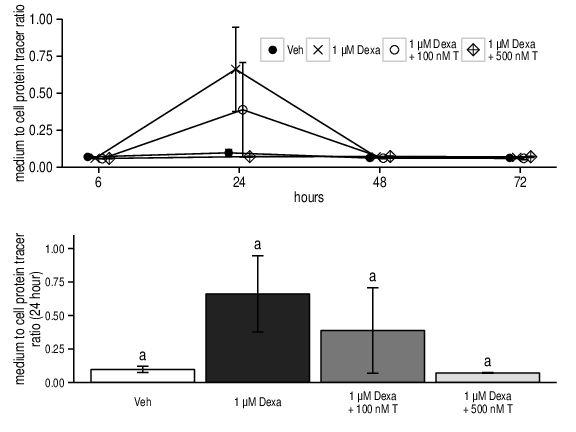
\includegraphics[width=6in,height=4.5in]{figure/proteindegradation-1} 

\end{knitrout}
%
\end{minipage} 

\protect\caption[Estimates of protein degradation rate in C2C12 myotubes treated with
Dexa with / without Testo.]{Estimates of protein degradation rate in C2C12 myotubes treated with
Dexa with / without Testo. (Top) Experimental timeline. (Middle) Ratio
of tracer in medium to tracer in cells, across time points. (Bottom)
Ratio of free tracer in medium to protein-bound tracer in cells, at
day 2 (n=5-6).\label{fig:protein-degradation-cells}}
\end{figure}


Preliminary experiments revealed that scintillation data were not
completely additive. In this experiment, the amounts of free tracer
from cell extract and protein-bound tracer in the medium proteins
are tens of times lower than the free tracer in the medium, and the
protein-bound tracer in the cells. In order to avoid addition of non-additive
data, protein degradation rate was estimated from the ratio of free
tracer in the cell culture medium to protein-bound tracer in the cell
extract (Fig. \ref{fig:protein-degradation-cells}, middle). However,
the results are essentially identical when free tracer from cell extract
and protein-bound tracer in the medium proteins are taken into account.
This scintillation-based method is semi-quantitative, meaning that
a doubling of the ratio of free tracer in the cell culture medium
to protein-bound tracer in the cell extract does not indicate a doubling
in protein degradation rate, but merely its upregulation.

Overall, due to sample size, the treatments were not statistically
significant across time points (ANOVA time X treatment, p = 0.401
for time; p = 0.259
for treatment). Nevertheless, the effects of the two steroids were
ample and dose-dependent at the 24 hour time point (ANOVA between
treatments, p = 0.144;
fig. \ref{fig:protein-degradation-cells}, bottom). For 24-hour vehicle-treated
cells, the ratio of free medium tracer to protein-bound intracellular
was 0.0968.
When cells received \SI{1}{\micro\molar}  Dexa, the ratio of free
medium tracer to protein-bound intracellular increased to 0.661
(Tukey's HSD vs. vehicle, p = 0.202).
Co-administration of Testo had a dose-dependent inhibitory effect
on protein degradation. When Dexa was supplemented with \SI{100}{\nano\molar}
Testo, the ratio of free medium tracer to protein-bound intracellular
was reduced to 0.388
(Tukey's HSD vs. Dexa alone, p = 0.776).
When Dexa was supplemented with \SI{500}{\nano\molar} Testo, the
ratio of free medium tracer to protein-bound intracellular was further
reduced to 0.0713
(Tukey's HSD vs. Dexa alone, p = 0.173).

A similar trend was recorded at the 48-hour time point. For 48-hour
vehicle-treated cells, the ratio of free medium tracer to protein-bound
intracellular was 0.062.
When cells received \SI{1}{\micro\molar} Dexa, the ratio of free
medium tracer to protein-bound intracellular increased to 0.0699
(Tukey's HSD vs. vehicle, p = 0.182).
Co-administration of \SI{100}{\nano\molar} Testo reduced the ratio
of free medium tracer to protein-bound intracellular to 0.0607
(Tukey's HSD vs. Dexa alone, p = 0.12).

Overall, Dexa myotube atrophy is correlated with an increase in tracer
release, indicating an upregulation of protein degradation. Testo
protection of myotubes is correlated with an inhibition of protein
degradation.


\section{Mechanisms of androgenic myoprotection in cultured myotubes treated
with dexamethasone}

In previous experiments, I established that loss of C2C12 myotube
protein during Dexa treatment is associated with an increase in protein
degradation at 24 hours after the initiation of steroid. Using a series
of chemical inhibitors, I investigated the molecular mechanisms that
could mediate this catabolic upregulation (Fig. \ref{fig:protein-degradation-cells-inhibitors},
top). As in the previous experiment, cells were differentiated over
7 days. In the final three days of differentiation, medium with tracer
was refreshed daily. For the final 24 hours, the tracer was removed,
and cells were treated with (A) vehicle, (B) \SI{100}{\nano\molar}
Dexa, or (C) \SI{100}{\nano\molar} Dexa and \SI{300}{\nano\molar}
Testo. In order to interfere with putative proteolytic pathways, other
sets of cells were treated with (D) \SI{100}{\nano\molar} Dexa and
\SI{25}{\micro\molar} chloroquine, an inhibitor of autophagy, or
(E) \SI{100}{\nano\molar} Dexa and \SI{5}{\micro\molar} MG132, an
inhibitor of the proteasome. Finally, in order to interfere with IGF-I
signaling, another set of cells were treated with (F) \SI{100}{\nano\molar}
Dexa, \SI{300}{\nano\molar} Testo, and \SI{50}{\nano\molar} picropodophyllin,
an inhibitor of IGF-1R.

\begin{figure}
\begin{minipage}[t][1.8in]{6in}%
\includegraphics[width=6in,height=1.8in]{12_media_dump_writingswork_draftthesis_artwork_cell-labeling-inhibitors.pdf}%
\end{minipage}

\begin{minipage}[t][4.5in][c]{6in}%
\begin{knitrout}
\definecolor{shadecolor}{rgb}{0.969, 0.969, 0.969}\color{fgcolor}
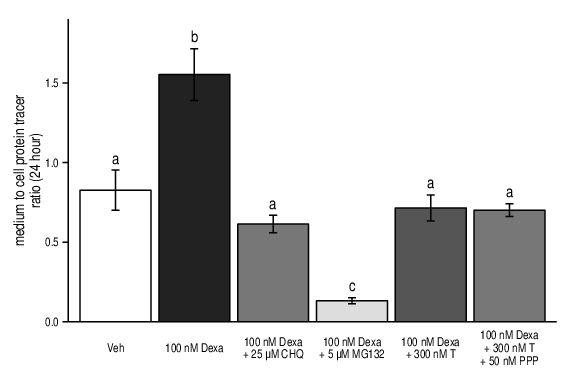
\includegraphics[width=6in,height=4in]{figure/inhibitors-1} 

\end{knitrout}
%
\end{minipage} 

\protect\caption[Interference of protein degradation in C2C12 myotubes treated with
Dexa with chemical inhibitors.]{Interference of protein degradation in C2C12 myotubes treated with
Dexa with chemical inhibitors. (Top) Experimental timeline. (Bottom)
Ratio of tracer in medium to tracer in cells (n=5-6).\label{fig:protein-degradation-cells-inhibitors}}
\end{figure}


The medium and the cells were fractionated as in the previous experiment.
Protein degradation rate was estimated via the ratio of free tracer
in the medium to protein-bound tracer in the cells. When cells were
treated with vehicle alone, the ratio of free medium tracer to protein-bound
intracellular was 0.826.
When cells received \SI{100}{\nano\molar} Dexa, the ratio of free
medium tracer to protein-bound intracellular increased to 1.55
(Tukey's HSD vs. vehicle, p = 0.000104).

The upregulation in catabolism was dependent on both proteasome and
lysosome actions. When the lysosome was inhibited with chloroquine,
the ratio of free medium tracer to protein-bound intracellular was
brought back to basal levels (0.614;
Tukey's HSD vs. Dexa, p = 1.44e-06).
However, proteasome inhibition had a more ample result, with the ratio
of free medium tracer to protein-bound intracellular depressed to
0.132
(Tukey's HSD vs. Dexa, p = 2.4e-10).

Testo repressed the upregulation of catabolism brought by Dexa to
basal levels (free medium tracer to protein-bound intracellular tracer
0.714;
Tukey's HSD vs. Dexa, p = 2.35e-05).
The protective effect of Testo was not apparently altered by the inhibition
of the IGF-1R pathway (free medium tracer to protein-bound intracellular
tracer 0.701;
Tukey's HSD vs. Dexa, p = 1).

Overall, in C2C12 cells, Dexa upregulates protein degradation, mainly
through the activation of the proteasome. Testo reverses the activation
of proteolysis in an apparently IGF-1R-independent manner, based on
the experimental sensitivity used in these assays.

\pagebreak{}


\chapter{Discussion}


\section{Testosterone alleviates dexamethasone-induced muscle atrophy in mice}

The present work investigated the molecular mechanisms mediating androgen
attenuation of GC-induced muscle atrophy in mouse. While the myoprotective
action of Testo was demonstrated in humans and rats, to date the role
of Testo in GC-mediated atrophy has not been studied in the mouse.
In fact, although some studies investigated transcriptional changes
in mouse muscle in response to Dexa, surprisingly few have described
macroscopic (organ level) atrophy.

In this dissertation, I demonstrated that a dose of \SI{10}{\milli\gram\per\kilo\gram\day}
Dexa induced a significant loss of muscle, as evidenced by decrements
in lean body mass and changes in the weight of individual muscles.
The effect was progressive, with the losses of lean body mass at day
3 being roughly half of the losses at day 7. The observed time dependence
is evidence for a Dexa-specific effect. As expected, lean body mass
was essentially unchanged in mice treated with vehicle alone. The
measurement of fat body mass indicated that the mice treated with
vehicle had essentially unchanged tissue fat during the experiment.
The unchanged lean and fat tissue content is evidence for the fact
that the experimental manipulations had no effect by themselves. The
robustness and quality of the study design of the study animals was
further supported by the fact that Dexa exerted its expected stimulatory
effect on accretion of body fat.

The observed change in total body mass was approximately equal to
that in lean body mass. This may explain why changes in body weight
(Fig. \ref{fig:Time-course-of-body-weight}), rather than body weight
at sacrifice (Fig. \ref{fig:Body-weight-at-sacrifice}), were significantly
altered by Dexa treatment. No other organ appeared to undergo atrophy
upon Dexa treatment. Dissection revealed no significant changes in
the size of viscera. No detectable changes were seen in the wet weight
of the heart (data not shown).

Gastrocnemius and quadriceps were the more sensitive muscles to Dexa,
whereas tibialis was essentially unchanged. The lack of response in
tibialis was surprising, given how common mouse tibialis manipulation,
such as electroporation of DNA, has been described in literature.
A report published during this work similarly failed to observe tibialis
anterior atrophy following 14 days treatment with a slightly lower
Dexa dose\citep{baehr2011muscle}. With 54\% fast glycolytic fibers
in gastrocnemius, compared to 59\% in tibialis anterior\citep{augusto2004skeletal},
the two muscles appear very similar in fiber type distribution. Therefore,
even if fiber typing was not evaluated in my model, it is unlikely
that differences in muscle sensitivity stem from differences in fiber
type. The lack of sensitivity in tibialis may have been due to the
fact that the tendinous component is weighing more in relative terms,
compared to large fleshy muscles.

There was a remarkable similarity between the first 3 days of the
in vivo experiment and the in vitro findings at 48 hour time point.
Whereas quadriceps lost 6\% of their weight, C2C12 myotubes lost about
5\% of their total protein upon Dexa treatment. This rate is similar
to that indicated by Desler for C2C12 myotubes that had been differentiated
over three days and then treated with Dexa\citep{desler1996effects}.

In contrast to the in vivo studies, the in vitro study could not have
been extended beyond the early days. Cells ability to thrive degraded
towards their third day of Dexa treatment, that is, their ninth day
of differentiation. The significant reduction in protein synthesis
seen at the 72-hour time point suggests that the cells became less
metabolically active compared to the 48-hour time point, perhaps due
to senescence. Therefore, the in vitro model appears inadequate beyond
the 48-hour time point. Moreover, the atrophic fibers' diameter becomes
comparable with that of the nucleus after the first two days (Fig.
\ref{fig:myotube-diameters}). Further reductions in cell diameter
would have required a shrinkage of the nucleus, which has not been
observed in the first two days of myotube atrophy. It was therefore
not possible to develop a longer term in vitro model of muscle atrophy.

Co-administration of Testo alleviated all macroscopic Dexa effects.
Similar to the profile of Dexa action, in absolute terms, the recovery
in lean body mass was approximately equal to that in total body weight.
The percentage by which total body weight, lean body mass, and individual
muscles recovered were similar, indicating that Testo action was limited
to muscle.

The experimental protocol may not have been ideal for observing the
time course for Testo action. On the one hand, the body weight changes
during the 7-day experiment (Fig. \ref{fig:Time-course-of-body-weight},
top) suggest that the protective action of Testo begins with the first
day of experiment. On the other hand, the time course was not reflected
in the individual muscle weight (Fig. \ref{fig:Muscles-weights}).
While 7-day samples appear effectively protected by Testo, 3-day samples
displayed a more limited anabolic response. This discrepancy may be
due to the fact that the mice analyzed in the 7-day study were slightly
more developed than those used in the 3-day sample. This was indicated
by the difference in levator muscles at sacrifice between vehicle-treated
animals at each time point. Moreover, the detection of the Testo protective
effect on muscle mass may be strained by its incomplete nature. Because
Dexa effect is progressive, its amplitude in the early stages is necessarily
small. When Dexa-induced atrophy is hard to detect, its incomplete
reversal will be even harder to demonstrate. I could not exclude a
temporal dissociation between the actions of the two steroids, as
the changes surrounding the acute onset of GAML were not investigated
in more detail, which was beyond the scope of this work. At the 7-day
time point, which is the more representative model of chronic glucocorticoid
myopathy, the alleviation of GAML has been well established.

The alleviation following Testo was incomplete in terms of lean body
mass and individual muscle weights. In contrast, total body weight
completely recovered. The source of this discrepancy remains unclear.
Dissection revealed no other viscera with an appearance of hypertrophy
following Testo co-administration. The dose of Testo used here was
shown to be effective in rats. However, the Dexa dose used in the
rat studies was much smaller, suggesting that mice studied here may
have benefited even more from an increased dose of Testo. Moreover,
mice may be intrinsically less responsive to Testo than rats, as the
former appear to be more resistant to many pharmacological treatments,
such as Dexa (reviewed here) or streptozotocin\citep{tay2005can}.
The most effective dose of Testo to fully prevent GAML should be pursued
in future studies. Within the limits of the present data, it may be
the case that no Testo dose would have overcomed the Dexa-induced
atrophy, which would then imply that atrophy inducing mechanisms of
Dexa potentially include pathways outside the scope of anabolic stimuli.

Notably, there were differences in the responsiveness to Testo between
muscle groups. Similar to Dexa sensitivity, an important component
appears to be the tendinous content. Levator ani is more responsive
to Testo than to Dexa, perhaps being explained by the increased presence
of AR compared to other muscles \citep{bentvelsen1996regulation}.
The apparent dependence of Testo response amplitude to the expression
of AR indicates that alleviation of GAML by AAS is a specific effect,
rather than an interaction at the GR level.

In vitro, myoprotective action of Testo was similarly present at late
time-points. The protection of C2C12 myotubes was dose-dependent,
based on the total protein assay. Paralleling the in vivo system,
the myoprotective effect in C2C12 cells was more pronounced when the
data were normalized to the first time point in the experiment (fig.
\ref{fig:protein-mass-cells} top versus bottom).


\section{Testosterone’s protective action was driven by the inhibition of
the dexamethasone-induced proteasome upregulation}

The mouse model of GAML largely replicated what was known from rat
experiments, where a strong upregulation of the proteasome system
is followed by alterations in protein synthesis.

In vivo, the E3 ligases also known as atrogenes were upregulated in
this model system. The upregulation of MuRF-1 was robust, and reached
statistical significance despite a small sample size. Upregulation
of MuRF-1 was confirmed at early stages in gastrocnemius, quadriceps,
and triceps (Fig. \ref{fig:Atrogenes-expression}; the latter not
shown). In agreement with published studies, the more specific ligase,
MAFbx, was upregulated by a lesser percentage than MuRF-1. In combination
with the practical limitations on sample sizes, the low-level activation
of MAFbx limited my ability to obtain statistical significance. Nevertheless,
the consistent trend across muscle groups of increased MAFbx expression
in response to Dexa indicates that the second atrogene was also part
of the atrophic transcriptional program. The massive proteasome upregulation
observed in day 3 samples increased the probability of the hypothetical
scenario in which protein degradation is limited by proteasome availability,
rather than E3 ligases. However, day 3 also marks the peak of proteasome
catalytic activity ( \ref{fig:Proteasome-enzymatic-activity}). The
synchronized stimulation of the proteasome and of the atrogenes indicates
that the proteasome - ubiquitin system may be at the center of GAML.

All these catabolic changes were inhibited by Testo co-administration.
In vitro, atrogenes expression was reduced to basal levels, and, in
the case of day 7 samples, even below baseline levels. The inhibitory
effect of Testo on MuRF-1 was predicted by the microarray study on
rat muscle. Similar to the rat study, the changes in MAFbx were also
in agreement with the phenotype, but of a lesser amplitude. In addition,
the proteasome activity was suppressed at its day 3 peak. This aspect
of muscle atrophy, already demonstrated as a component of male post-castration
muscle atrophy\citep{serra2013effects}, has never been investigated
in GAML, nor in its attenuation by Testo.

Upregulation of proteasome activity, independent of atrogene status,
has been reported by others\citep{baehr2014muscle}. It is unclear
how Dexa achieves this upregulation. In this study, limited evaluation
of transcripts for proteasome subunits A6, B10, or D4 were inconclusive
(data not shown).

In vitro, proteasome inhibition led to nearly complete suppression
of proteolysis, beyond the basal levels seen in vehicle-treated cells.
This finding indicates that most of the proteolytic activity in C2C12
cells is dependent on the proteasome.

A study by Baehr and colleagues\citep{baehr2011muscle}, which was
published while my experiments were under way, showed that MAFbx knockout
did not reduce the amplitude of GAML, while MuRF-1 knockout reduced
GAML to about half of its amplitude in wild-type mice. My data show
that, instead of rejecting the proteasome-centered model of GAML,
future studies should focus on finding alternative ways by which the
proteasome promotes catabolic activity. For example, the simplest
scenario fitting today's data is one where the proteasome performs
the clearance of the bulk of dispensable proteins. An alternative
explanation, which takes into account the subsiding evolution of the
atrogene surge, is that atrogenes ubiquitinate, and target for degradation,
a yet unidentified myoprotective intracellular factor, thus unleashing
a cascade of proteasome-independent mechanisms. Some limited attempts
to detect multiple ubiquitination states for MuRF-1's putative substrate,
myosin heavy chain, were inconclusive (data not shown). If MuRF-1
has only this limited and limiting action, disruption of MuRF-1 in
Baehr's knockout mice could have been supplanted by partially homologous
genes, such as MuRF-2 or Fbxo40\citep{shi2011scf-fbxo40,witt2005murf-1}.
The distinction between the two scenarios is difficult, especially
in the in vivo approach. In either scenario, the role of the proteasome
is indispensable for GAML. Nevertheless, proteasome inhibition by
Testo co-administration emerges from this work as an important mechanism
of GAML alleviation.

The experiments performed in this study clearly exclude a role for
the autophagosome - lysosome system in digestion of bulk myofiber
proteins. The in vivo data indicate a persistent suppression of autophagy-related
genes across muscle groups and time points. Moreover, lysosome-associated
cathepsin L enzymatic activity is suppressed by Dexa in a statistically
significant manner at all time points. The downregulation of cathepsin
activity and expression was more ample than the loss of muscle protein,
indicating that an active process of cathepsin degradation is activated
by Dexa in vivo. 

The finding of Dexa-induced downregulation of autophagy was unexpected.
Some atrophic conditions, most notably starvation, lead to autophagy
regulation. The rat microarray findings found cathepsin L among the
set of genes upregulated by Dexa. Even in this study, a narrow measurement,
the accumulation of lipidated LC3 appeared upregulated by Dexa (Fig.
\ref{fig:LC3-hyperlipidated}, middle). However, the microarray results
were never validated by qRT-PCR. In the present work, when the hyperlipidated
LC3 form is normalized to its precursor, its levels appeared essentially
unchanged in response to Dexa (Fig. \ref{fig:LC3-hyperlipidated},
right). The accumulation of LC3 protein, both in precursor and mature
form, indicates reduced capacity in the autophagolysosome compartment,
especially in the present context of downregulated LC3 protein expression.
This line of evidence corroborates the downregulated enzymatic activity
to collectively exclude a putative role for autophagy in bulk GAML.

Intuitively, it is more likely for bulk protein catabolism to be mediated
by the smaller proteasome and atrogenes than the larger autophagosome.
However, autophagy may play a regulatory, initiating role in GAML.
In the in vivo studies, the amplitude and invariability of autophagy
inhibition prove its modulation by Dexa. One could speculate that
such changes, ampler than those in muscle mass, cannot be simple inconsequential
side effects. While the present data solidly exclude a role for bulk
protein digestion, further studies are needed to elucidate which proteins
are spared from autophagy during GAML, and what is the regulatory
effect of their sparing from autophagy.

While the in vivo data suggested that downregulation of autophagy
is part of GAML, I found the opposite phenomenon in cell culture experiments.
There, inhibition of lysosomes with chloroquine had a significant
protective effect. The differences between the in vivo and in vitro
data underscore the limitations intrinsic to cell culture models.
Many factors absent from the cell culture experiment may explain the
observed contrast, including myoprotective influences of the motor
neuron at neuromuscular junctions and vascularization of muscle tissue.
Moreover, the advanced quiescence of the cultured myotubes contrasts
with the ample in vivo ability for muscle to regenerate. Given the
reductionism of the culture cell experiment, the in vivo experiment
is likely more reflective of what occurs in human glucocorticoid myopathy.
The fact that Testo reversed most of the in vivo effects of Dexa on
autophagy suggests that this pathway may be relevant for GAML attenuation.

Prior to this work, the calpain system was the least likely effector
of GAML. In agreement with the literature, this study could not substantiate
Dexa-induced changes in calpain enzymatic activity, calpain, or calpastatin
protein levels (data not shown). Overall, the absence of Dexa-induced
amplification in catabolic activity in the cathepsin and calpain pathways
reduces the scope for AAS myoprotection through inhibition of these
pathways. Moreover, Testo had no reliable effect on the Dexa-induced
changes in the autophagosome - lysosome pathway. Therefore, Testo
protection is unlikely to be mediated by inhibition of cathepsin or
calpain.

Studies on protein synthesis rate have been strained by the limited
technical abilities of measuring protein synthesis in mice. No study
that I am aware of measured changes in the rate of protein synthesis
in mice prior to this work. The studies on rats indicated that such
measurements are fraught with high variability, and would therefore
likely fail to detect any effect. I did not measure protein synthesis
directly in vivo. The measurements of protein synthesis rate in vitro
failed to identify any significant change in response to Dexa. C2C12
cells are surprisingly dependent on protein synthesis, with either
translational inhibitor cycloheximide and puromycin leading to cell
death and detachment within hours (data not shown). Overall, the lack
of detectable changes in protein synthesis rate agrees with findings
in rat L6 cells \citep{menconi2008dexamethasone} and explanted muscle
experiments\citep{dardevet1998glucocorticoid}.

In order to detect subtle changes in protein synthesis, I investigated
a series of its regulators. I failed to identify changes in levels
of phosphorylated eIF2α and eIF3f in response to either Dexa or Testo
(Figs. \ref{fig:Phosphorylated-eif2}, \ref{fig:eif3f}). I could
not detect ATF4 protein in muscle lysates (data not shown). In the
7-day samples, both total and phosphorylated 4E-BP were upregulated
by Dexa. With these data, it was unclear whether the active negative
regulator of protein synthesis, unphosphorylated 4E-BP was increased
or decreased by chronic Dexa exposure. The changes in total and phosphorylated
4E-BP induced by Testo are small, and would be unlikely to lead to
increased inactivation of 4E-BP. Therefore, based on these data and
the limitations of the model system, there was no evidence that, at
7-day time point, that the protective action of Testo benefited from
increased protein synthesis.

While the reported experiments were ongoing, Baehr and colleagues
reported that Dexa decreased protein synthesis rate at day 3 and increased
it at day 14 in mouse triceps\citep{baehr2011muscle}. Baehr et al.
findings suggest that acute Dexa represses protein synthesis, whereas
chronic Dexa is associated with a compensatory restoration of translational
capacities. At the 7-day time point analyzed in this study, a measurement
of protein synthesis by Baehr’s method would have been indecisive,
as the muscle would have been midway in the switch from a low to high
translation rate.

In conclusion, Testo induced muscle protection through multiple mechanisms,
among which inhibition of the proteasome system stood out by amplitude
and persistence.


\section{Molecular mechanisms linking dexamethasone and testosterone to protein
metabolism}

In agreement with the rat studies, the present work demonstrates that
Dexa-induced upregulation of atrogenes is coordinated with increased
expression of Foxo transcription factors (Fig. \ref{fig:Foxo-expression},
top). A Foxo3a surge was even more robust than the increase in MuRF-1,
with a statistically significant presence in day 1 samples. Moreover,
the transcription factor Klf15, which is a target of Foxo, and their
synergistic partner in the upregulation of MuRF-1, underwent an equally
rapid intensification (Fig. \ref{fig:Foxo-expression}, bottom).

In addition to repression of atrogenes, Testo reverses other actions
of Dexa. This efficient, multi-directional action of Testo suggests
that it may act on a higher-level mediator of GAML. Two molecular
levers responded in a uniform, consistent manner to the two steroids,
and therefore may be high-level mediators of AAS and GC. The first
is REDD1 / Ddit4, the negative regulator of mTORC1. Dexa consistently
upregulated REDD1 expression in samples from days 1, 3, and 7. The
amplitude of upregulation decreased with time. A time course where
Dexa amplifies REDD1 only for the first week could explain Baehr's
observations on protein synthesis changes during GAML. As REDD1 inhibition
of mTORC1 subsides, the 4E-BP-mediated brake on protein synthesis
is gradually reduced. Testo co-administration reversed REDD1 upregulation
to a significant degree at 7-day time point, when Dexa-induced amplification
was at its lowest. Further experiments are needed to analyze the relationship
between REDD1 and protein synthesis, especially at later time points,
which have not been investigated here.

The transcriptional upregulation of Foxo by Dexa may have been compounded
by Akt inhibition. GC caused a large decrement in Ser 473 phosphorylation
of Akt (Fig. \ref{fig:Akt-phosphorylation}), which in turn is expected
to protect Foxo from export to cytosol and proteasome-mediated destruction.
AAS had no apparent effect on Ser 473 phosphorylation. The discrepancy
between Ser 473 phosphorylation and muscle recovery may be explained
within the model described by Britto\citep{britto2014redd1}, who
showed preliminary evidence that Ser 473 is not involved in Akt inactivation
during GAML. Another explanation is based on the ability of Dexa to
disconnect Akt from insulin and IGF-I signals (discussed in a dedicated
section). The only other trait shared between mice receiving Dexa
with versus without Testo is accumulation of fat mass, suggestive
of whole-body insulin resistance. At the level of muscle, Dexa induces
insulin resistance by interference at IRS 1 and p85 levels.

The other reliable change in GAML and its alleviation by Testo was
observed in IGF-I expression. In agreement with studies on rats, Dexa
reduced IGF-I expression, while Testo co-administration restored reduced
IGF-I expression to basal levels (Fig. \ref{fig:Igf1-expression}).
In agreement with all previous studies, I could not substantiate changes
in the phosphorylation of IGF-1R that would correlate with the IGF-I
upregulation (data not show). It is unclear to what extent IGF-I would
mediate AAS myoprotection given the aforementioned interference by
Dexa at IRS 1 and p85.

In vitro, I attempted to gauge the role of IGF-1R in Testo myoprotection.
A novel IGF-1R inhibitor, picropodophyllin, had no effect on Testo
protection. However, the same experiment uncovered a series of other
shortcomings of the cell culture experiment, including a higher reliance
on autophagy compared to the in vivo model. Better causal inferences
could be made by employing in vivo transgenic models of interference
within the IGF-I / Akt / mTORC1 axis.


\section{Future directions}

This work demonstrates that Testo protects mouse muscle in vivo and
in vitro by reversing the Dexa-induced upregulation of proteasome
activity. On the other hand, the set of E3 ligases that cause GAML
is incomplete. The role of candidates such as Fbxo40 remains to be
investigated. Future studies will need to determine whether Testo
suppresses the other E3 ligases.

At this time, the mechanisms by which Dexa upregulates Foxo transcription
factors is a subject of speculation. Even less is known about the
way in which Testo represses Foxo. Chromatin immunoprecipitation tests
using Foxo promoters would help resolve this question.

The in vivo experiment suggest that Testo also reversed Dexa-induced
repression of autophagy. The role of autophagy in GAML would be better
understood by observing the effects of GC and AAS on muscle from LC3-GFP
transgenic mice.

Both autophagy and protein synthesis appeared to have changed in time,
during the in vivo experiment. Because they were performed as three
independent experiments, an ability to infer the time course of changes
was limited. A direct exploration of time-dependent changes is required,
in order to establish which changes in protein metabolism are late-onset,
reactive adjustments.

I was not able to observe the effect of IGF-I modulation, due to an
overarching suppressive effect of Dexa which disconnects the transmembrane
receptors from their Akt effector. The mechanisms by which Dexa achieve
this disconnection are largely the subject of speculation. Future
studies that establish if and how GR interferes with the IGF-I / Akt
pathway are needed.

Transgenic models, such as the triple Foxo knockout, are needed, in
order to determine the relative importance and the eventual interaction
between Foxo and the mTOR pathway. 


\section{Conclusions}

Testo co-administration attenuates the loss of muscle mass induced
by GC administration in mice. Based on the model systems used in this
thesis, Testo myoprotection was exerted through an inhibition of the
proteasome, mediated by Foxo and REDD1. Changes in these, as well
as in IGF-I intramuscular expression, indicate that the two classes
of steroids counter each other’s effect on the Akt signaling pathway
(Fig. \ref{fig:Mechanisms-of-AAS}). AAS therapy may be beneficial
for a subset of male adult patients receiving chronic GC as a treatment,
especially if they present with biochemical and clinical signs of
hypogonadism. The relative importance of the proteasome in glucocorticoid
myopathy suggests that in addition to Testo, other more direct proteasome
inhibitors such as bortezomib, may be useful as adjunctive therapy.

\begin{figure}
\includegraphics[width=6in,height=5in]{13_media_dump_writingswork_draftthesis_artwork_conclusion.pdf}\protect\caption{Mechanisms of AAS alleviation of GAML\label{fig:Mechanisms-of-AAS}}


\end{figure}


\begin{singlespace}
\pagebreak{}
\end{singlespace}

\bibliographystyle{15_media_dump_writingswork_draftthesis_nihunsrt}
\phantomsection\addcontentsline{toc}{chapter}{\bibname}\bibliography{14_media_dump_writingswork_draftthesis_thesis}


\begin{singlespace}
\pagebreak{}
\end{singlespace}


\chapter{Curriculum vitae}


\section*{Nicolae Lucian Sandor}


\subparagraph*{Education}
\begin{itemize}
\item PhD candidate, Boston University School of Medicine, expected graduation
2015
\item BS (Licentiat in Biofizica), Universitatea Bucuresti, 2005
\item BM\textbackslash{}DM (Doctor in Medicina), Universitatea de Medicina
si Farmacie Carol Davila Bucuresti, 2002
\end{itemize}

\subparagraph*{Research experience}
\begin{itemize}
\item 2012-2015: Department of Medicine, Boston University School of Medicine,
P.I. Dr. Shalender Bhasin, under the supervision of Drs. Carlo Serra
and Monty Montano

\begin{itemize}
\item Subject: Testosterone alleviating glucocorticoid-induced muscle loss.
\end{itemize}
\item 2009-2012: Department of Biophysics, Boston University School of Medicine,
P.I. Dr. Assen Marintchev

\begin{itemize}
\item Subject: Interactions between translation initiation factors eIF1A
and eIF5B
\end{itemize}
\item 2005-2008: Center for the Study of Brain, Mind and Behavior, Princeton
University, P.I. Dr. Anne Treisman, FRS

\begin{itemize}
\item Subject: Brain mechanisms for statistical processing of visual scenes
\end{itemize}
\item Summer 2004: Biology Department, Universitatea Bucuresti, P.I. Dr.
Gordon Reid, under the supervision of Dr. Iurie Barbu

\begin{itemize}
\item Subject: The mediation of thermoception by ionic membrane channels
\end{itemize}
\item 2001-2002: Biophysics Department, Universitatea de Medicina si Farmacie
Carol Davila Bucuresti, P.I. Dr. Dan Eremia, under the supervision
of Dr. Eva Katona, 

\begin{itemize}
\item Subject: The effect of non-ionizing radiation of the mobility of the
cell membrane lipids
\end{itemize}
\end{itemize}

\subparagraph*{Peer-reviewed publications}
\begin{enumerate}
\item Serra C, Tangherlini F, Rudy S, Lee D, Toraldo G, Sandor NL, Zhang
A, Jasuja R, Bhasin S. \emph{Testosterone improves the regeneration
of old and young mouse skeletal muscle}. J Gerontol A Biol Sci Med
Sci. 2013 Jan;68(1).
\item Serra C, Sandor NL, Jang H, Lee D, Toraldo G, Guarneri T, Wong S,
Zhang A, Guo W, Jasuja R, Bhasin S. \emph{The effects of testosterone
deprivation and supplementation on proteasomal and autophagy activity
in the skeletal muscle of the male mouse: differential effects on
high-androgen responder and low-androgen responder muscle groups}.
Endocrinology. 2013 Dec;154(12).
\item Guo W, Bachman E, Vogel J, Li M, Peng L, Pencina K, Serra C, Sandor
NL, Jasuja R, Montano M, Basaria S, Gassmann M, Bhasin S. \emph{The
effects of short-term and long-term testosterone supplementation on
blood viscosity and erythrocyte deformability in healthy adult mice}.
Endocrinology. 2015 Mar 16;en20141784. PMID: 25774550.
\end{enumerate}

\subparagraph*{Other scientific communications}
\begin{enumerate}
\item Sandor NL, Hendrickson E, Sandor D, Wagner G, Pestova TV, Marintchev
A. \emph{Interplay between intra- and intermolecular interactions
involving human eIF1A and eIF5B}. Abstract presented at the 2010 Meeting
of Translational Control, Sept. 2010, Cold Spring Harbor, NY.
\item Sandor NL, Lee D, Toraldo G, Zhang A, Jasuja R, Bhasin S, Serra C.
\emph{The role of testosterone on the control of muscle protein synthesis
and degradation}. Abstract presented at the 2011 Evans Center Days,
Nov. 2011, Boston, MA.
\item Serra C, Lee D, Sandor NL, Toraldo G, Jang H, Jasuja R, Bhasin S.
\emph{Characterization of the neuromuscular junction in castrated
male mice}. Poster presented at ENDO2013, The Endocrine Society's
95th Annual Meeting \& Expo, 2013, San Francisco, CA.
\item Sandor NL, Jasuja R, Serra C, Bhasin S. \emph{Testosterone alleviates
glucocorticoid myopathy by inhibiting the proteolytic machinery}.
Poster presented at the 2013 Evans Center Days, Nov. 2013, Boston,
MA.\end{enumerate}

\end{document}
